\documentclass[13.5pt]{extarticle}
\usepackage[UTF8,fontset=fandol]{ctex}
\IfFontExistsTF{Times New Roman}
    {\setmainfont{Times New Roman}}
    {\IfFontExistsTF{TeX Gyre Termes}{\setmainfont{TeX Gyre Termes}}{}}
\usepackage[a4paper,left=2.5cm,right=2.5cm,top=2.5cm,bottom=2.5cm]{geometry}
\usepackage{xcolor}
\definecolor{changeblue}{RGB}{0,82,170}
\newcommand{\changed}[1]{{\color{changeblue}#1}}
\newenvironment{changehighlight}{\par\begingroup\color{changeblue}}{\par\endgroup}
\usepackage{hyperref}
\usepackage{xurl}
\Urlmuskip=0mu plus 2mu
\usepackage{booktabs}
\usepackage{longtable}
\usepackage{graphicx}
\newcommand{\tabrowrule}{\hline}
\newcommand{\frameworkcell}[1]{\raisebox{-3.0\baselineskip}[0pt][0pt]{\parbox{0.13\textwidth}{\raggedright\arraybackslash #1}}}
\usepackage{tabularx}
\usepackage{array}
\usepackage{enumitem}
\usepackage{titlesec}
\usepackage{microtype}
\usepackage{float}
\usepackage{caption}
\usepackage{setspace}
\usepackage[backend=biber,style=ieee,sorting=none]{biblatex}
\addbibresource{sections/references.bib}

\hypersetup{
    colorlinks=true,
    linkcolor=black,
    urlcolor=blue,
    citecolor=blue
}
\captionsetup{
    font={scriptsize,stretch=1.5},
    labelfont={bf},
    textfont={rm},
    labelsep=quad
}
\setlist{nosep,leftmargin=1.8em}
\setcounter{secnumdepth}{0}
\setcounter{tocdepth}{2}
\titleformat{\section}{\Large\bfseries}{ }{0pt}{}
\titleformat{\subsection}{\large\bfseries}{ }{0pt}{}
\titleformat{\subsubsection}{\normalsize\bfseries}{ }{0pt}{}
\let\oldsection\section
\renewcommand{\section}{\clearpage\oldsection}
\renewcommand{\abstractname}{%
    \fontsize{16}{0}\selectfont
    摘\nolinebreak\hspace{\ccwd}要
    \vspace{0.5cm}
}

\begin{document}

\begin{titlepage}
    \centering
    \vspace*{2.5cm}

    {\Huge \textbf{面向协作边缘计算场景的 LLM 推理优化：算法研究与应用综述}} \\[1.2cm]
    {\Large Collaborative Edge Computing for LLM Inference: Algorithms and Applications} \\[3.2cm]

    \begin{center}
        {\fontsize{14}{0}\selectfont \textbf{研究综述报告}} \\[0.5cm]
        {\fontsize{12}{0}\selectfont \textbf{协作边缘计算赋能的大模型推理优化}}
    \end{center}

    \vfill

    \begin{center}
        \begin{tabular}{ll}
            \textbf{版本：} & \textbf{v2.0} \\
            \textbf{日期：} & \textbf{2026年8月} \\
        \end{tabular}
    \end{center}

    \vspace{1.5cm}
\end{titlepage}

\clearpage
\setstretch{1.75}

\begin{abstract}
大语言模型（LLM）推理正从云端集中式服务逐步向网络边缘迁移，以满足低时延、高带宽效率及数据隐私等需求。然而，单个边缘节点（如基站、边缘服务器、边缘网关）受限于计算、存储和通信资源，难以独立承载完整的大模型部署。协作边缘计算（CEC）通过将地理分布、能力异构的终端设备、边缘服务器及 AI 加速板卡整合为统一的协作资源池，为突破这一瓶颈提供了可行路径。在 CEC 框架下，模型切分、请求调度、键值（KV）缓存与上下文管理、服务路径选择等关键环节均可跨节点联合优化。然而，边缘场景下算力异构，资源受限，动态网络条件和请求，以及用户移动性等特性给LLM推理系统带来了新的研究挑战。

\par 本文围绕 CEC 场景下的大语言模型推理优化展开综述。首先，本文梳理 LLM inference 的基本执行机制、问题空间和“优化对象--执行范围”分类框架，并分析 CEC 相较云侧集中式 serving 新增的资源、网络、状态和移动性约束。在此基础上，本文重点讨论三类算法问题：\textbf{资源自适应模型切分部署、业务感知 batching，以及用户移动场景下的请求卸载与状态管理}。相关工作部分覆盖 layer、tensor、expert、prefill阶段和decoer阶段分离等切分方式；动态组批与 chunked prefill 等 batching  调度机制; 以及 request/session routing、context/KV/runtime state migration 和 multi-agent workflow orchestration 等请求调度方法。面向验证环境，报告进一步给出三项具体方案：以统一代价模型比较 TP、PP 和 PP+TP，并采用动态规划求解非均匀 PP 分割；以 CMDP 建模并采用带长期风险约束和安全投影的 Safe-RL 调节 batching策略，以确保不违反 SLO 约束；联合选择请求执行节点和 KV 获取方式，优化移动会话的长期服务成本。最后，本文讨论三类算法的协同关系及其在 Ascend 和 vLLM-Ascend 基础设施上的实现与评估方法。
\end{abstract}

\clearpage
\tableofcontents
\clearpage

\phantomsection
\section*{一、引言}
\addcontentsline{toc}{section}{一、引言}

\phantomsection
\subsection*{1.1 研究背景与应用动机}
\addcontentsline{toc}{subsection}{1.1 研究背景与应用动机}

大语言模型推理的部署正在从云端集中式服务扩展到多个边缘节点参与的协作式服务。现有优化研究主要覆盖两类环境：端侧推理通过模型压缩、量化、小模型和端侧 NPU/GPU 加速，使部分请求能够在用户设备上完成；云端或数据中心推理服务则通过高性能算子、连续批处理、KV Cache 管理、模型并行和多实例调度提高吞吐并降低尾时延。已有系统与综述分别从执行运行时、内存管理、批处理调度和分布式服务等角度总结了这些机制 \cite{yu2022orca,kwon2023efficient,agrawal2024taming,zhong2024distserve,zheng2024sglang}, \cite{zhou2024survey,zhen2025taming,pan2025survey}。

两类环境各有适用边界。端侧推理具有低时延和数据本地性优势，但受算力、内存、功耗和散热限制，难以长期承载复杂大模型和高并发服务。云侧推理资源充足、框架成熟，但网络传输会影响端到端时延、带宽消耗、隐私边界和服务可用性。与此同时，基站、网关、园区和近用户位置已经部署了大量分散、异构且动态变化的边缘算力；这些资源规模大于单个端侧设备，又缺少数据中心同构集群的稳定互联与统一规格。

本文所讨论的 CEC（Collaborative Edge Computing，协作边缘计算）将地理分布、能力异构的终端设备、边缘服务器和 AI 板卡组织为协作资源池，并借助 Wi-Fi 接入点、路侧单元、5G 基站和网关等基础设施交换请求、中间结果与运行时状态。如图~\ref{fig:collaborative-edge-computing} 所示，多个边缘资源可以共同完成模型部署和推理执行，请求路径不依赖预设的端、边、云三级结构。终端可以作为请求入口或计算节点，CEC 不是为了替代中心化的云，而是作为补充，外部云服务则在业务允许时作为可选服务或异常回退路径。分布式协同智能研究为异构资源、链路和服务位置的联合优化提供了参考 \cite{duan2022distributed}；本文聚焦协作边缘资源池内部的模型切分、请求调度和状态管理。相应的系统问题是：如何在资源与网络持续变化的条件下，以可控成本满足业务时延、吞吐、服务连续性和数据隐私要求。

\begin{figure}[htbp]
    \centering
    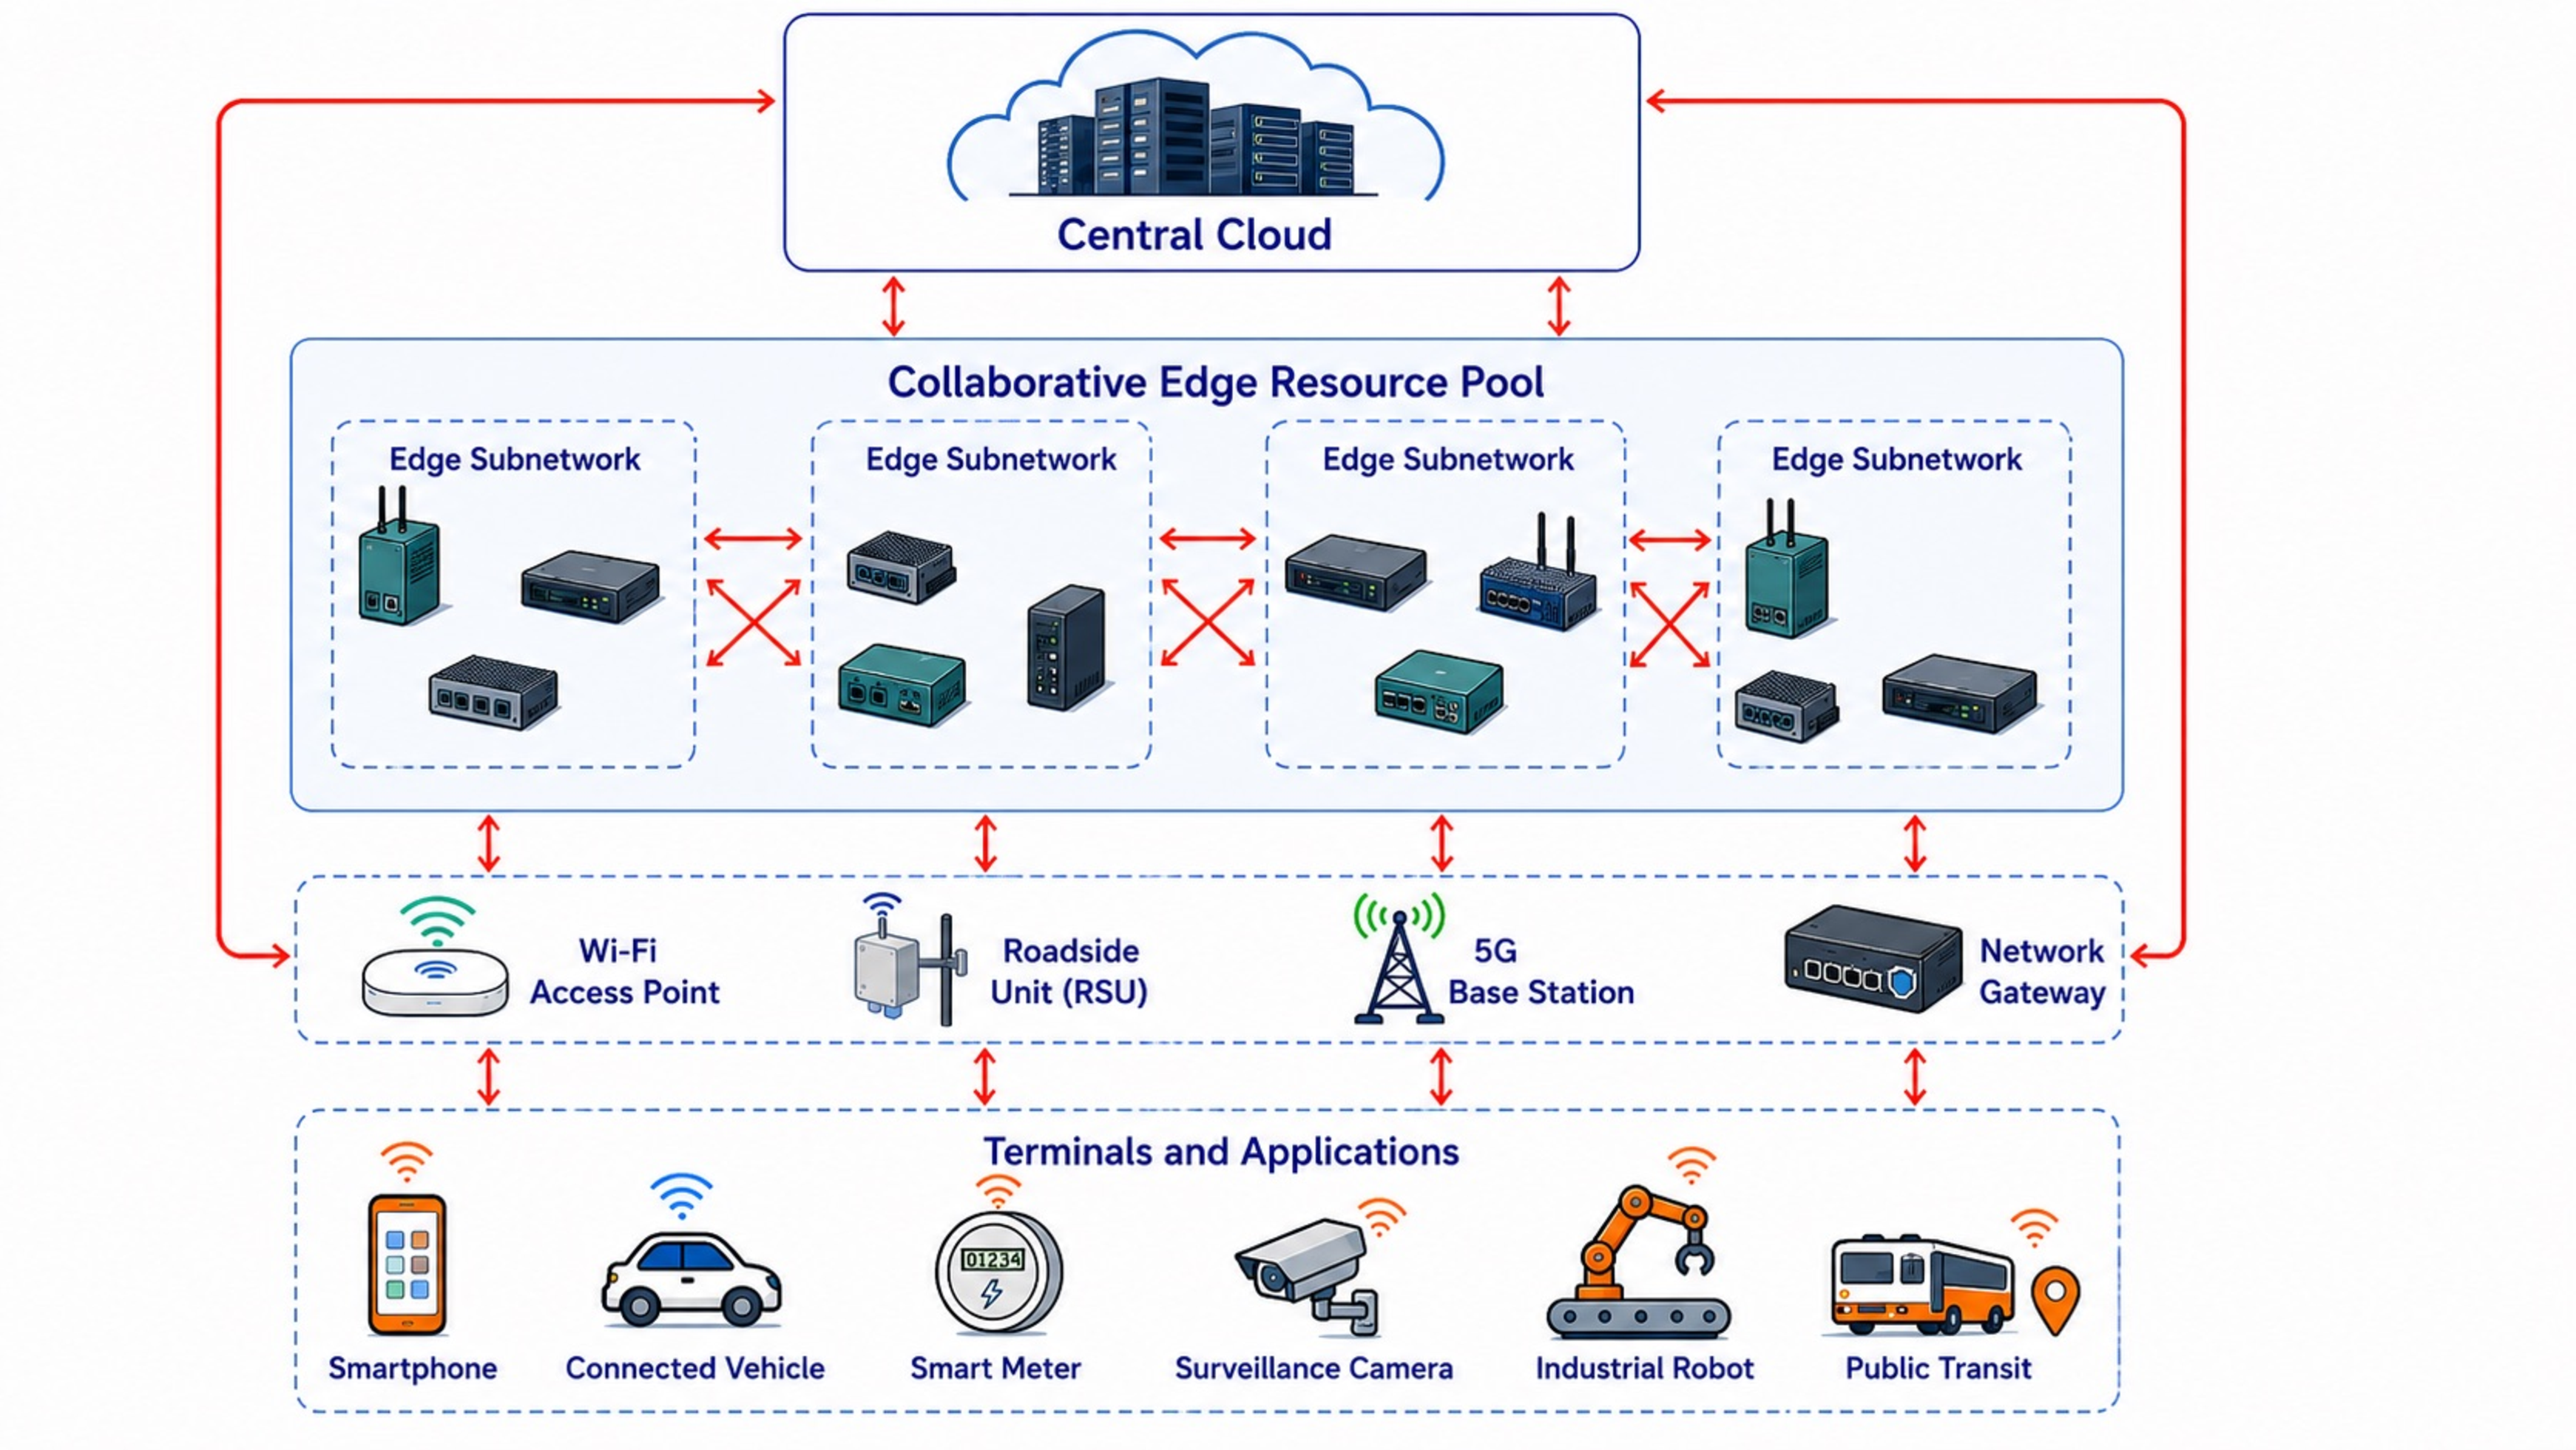
\includegraphics[width=\textwidth]{figures/ch1_collaborative_edge_computing.pdf}
    \caption{\textbf{协作边缘计算示意图。}协作边缘计算汇聚泛在、地理分布设备的计算资源以共同执行计算任务，从而扩展可用资源池，实现低时延数据处理、灵活设备接入与更广的服务覆盖。}
    \label{fig:collaborative-edge-computing}
\end{figure}



\phantomsection
\subsection*{1.2 CEC 场景下边缘 LLM 推理的关键挑战}
\addcontentsline{toc}{subsection}{1.2 CEC 场景下边缘 AI 推理的关键挑战}
然而，CEC场景给 LLM 推理带来了新的挑战，具体如下

\textbf{CEC 场景下的边缘 AI 推理首先受到资源异构和碎片化的约束。}终端设备以及部署在基站、网关、园区和边缘服务器中的 GPU、NPU 与 AI 板卡，在算力、内存、显存、功耗预算和加速库支持上差异显著，模型部署不能直接套用数据中心中“节点规格相近、互联稳定、控制面统一”的假设。同一个模型在不同硬件上可能面临完全不同的显存瓶颈、算子支持和通信代价，部署策略也必须随资源状态动态调整。

\textbf{LLM 推理本身还具有显著的状态和内存压力。}Prefill 阶段会为后续 decode 生成 KV Cache，decode 阶段又会随着输出长度不断追加状态；在长上下文、多轮会话和高并发场景中，KV Cache、prefix cache 和 session state 会长期占用显存，并要求系统管理其生命周期、位置和一致性。一旦这些状态跨节点访问、迁移或重算，通信成本、服务连续性和隐私边界都会同时受到影响。

\textbf{请求动态性进一步放大了调度难度。}用户并发数、prompt 长度、输出长度、请求复杂度和时延 SLO 都在持续变化，边缘节点又常常缺乏云侧的大规模请求池，静态 batching、固定 batch size 和固定服务路径难以稳定满足业务要求。对于移动用户，接入点和合适的服务实例还会随位置变化；距离最近的节点未必具有最短的排队时间或端到端时延。若用户会话中的 KV 或上下文状态仍保留在原服务节点，服务切换还可能引发状态迁移、远程访问或重新 prefill。

这些因素相互影响：模型切分会改变各节点的计算量和跨节点 activation 传输，batching 会改变排队时间、KV 占用和设备利用率，请求卸载又会改变流量分布与状态位置。因而，CEC LLM inference 需要联合比较计算收益、通信开销和状态迁移成本，并在业务时延、隐私和服务连续性约束下选择可执行的部署与调度方案。


\phantomsection
\subsection*{1.3 相关研究基础与问题主线}
\addcontentsline{toc}{subsection}{1.3 相关研究基础与问题主线}

现有研究为 CEC LLM inference 提供了多方面基础。一方面，on-device inference 关注模型压缩、低比特执行、小模型设计和端侧硬件加速，使部分请求能够在用户设备本地完成；FlexGen~\cite{sheng2023flexgen}、Petals~\cite{borzunov2023petals}、HexGen~\cite{jiang2023hexgen} 等工作则进一步展示了资源受限或异构环境下的大模型推理可以通过分层存储、协作式 block 放置和异构并行来突破单节点容量限制。另一方面，cloud/datacenter LLM serving 已经围绕 continuous batching、PagedAttention、chunked prefill、prefill/decode disaggregation、KV cache management 和多实例调度形成了较成熟的系统路线，Orca~\cite{yu2022orca}、vLLM~\cite{kwon2023efficient}、Sarathi-Serve~\cite{agrawal2024taming}、DistServe~\cite{zhong2024distserve}、SGLang~\cite{zheng2024sglang} 和 Mooncake~\cite{qin2025mooncake} 等系统分别代表了不同层面的关键机制。

边缘计算领域长期研究任务卸载、资源分配、移动性管理和网络感知调度，其中许多卸载模型将任务描述为具有固定输入大小、计算量、deadline 和能耗约束的作业。LLM 推理的服务时间还取决于 prompt、输出长度、decode 进度、batch 组成和 KV 状态，复杂请求也可能涉及多模型、多智能体或多阶段执行。因此，CEC LLM 推理同时包含 LLM serving 中的 prefill/decode、KV Cache、batching、推测解码和分布式执行问题，以及协作边缘环境中的资源异构、动态网络、用户移动、隐私约束和服务连续性问题。

基于这一交叉特征，本文将相关工作组织为三条主线。第一条是 \textbf{CEC 下的资源自适应模型部署方法}，关注模型结构、模型组件和推理阶段如何在异构协作节点之间切分与放置。第四章的综述覆盖 layer、tensor、expert、推理阶段和生成职责等不同切分对象，面向验证环境的具体方案则先比较 TP、PP 和 PP+TP，再采用动态规划求解非均匀 PP 的连续 layer 分割。第二条是 \textbf{CEC 中的业务感知 batching 参数优化算法}，关注请求进入推理实例后如何根据 SLO、队列状态、KV 占用和 prefill/decode 干扰选择 batch 形成与更新策略，具体方案采用 Safe-RL 联合调节 batch 参数、请求顺序和运行时机制。第三条是 \textbf{CEC 中的 LLM inference task offloading}，关注完整请求、会话、multi-agent workflow 以及 context/KV/runtime state 如何在协作边缘节点之间路由、卸载、迁移和复用。这三条主线分别对应模型部署、实例内调度和跨节点服务路径选择。


\phantomsection
\subsection*{1.4 研究范围与内容组织}
\addcontentsline{toc}{subsection}{1.4 研究范围与内容组织}

本文聚焦 \textbf{CEC 场景下的大语言模型推理优化问题}。研究范围限定在推理阶段，不讨论大模型训练、预训练或微调过程；重点关注终端设备、边缘服务器、AI 板卡以及部署在基站、网关和园区中的推理节点之间的大模型推理协同，包括资源自适应模型切分与部署、动态 batching、prefill/decode 调度、分布式 KV/状态管理、任务卸载、请求路由、移动性感知调度和服务连续性保障。


底层算子优化、硬件实现和模型结构设计仅在影响 CEC 推理系统时纳入讨论。例如，低比特算子会影响模型能否部署到目标设备，KV Cache 布局会影响状态迁移和缓存复用，便于切分的模型结构会影响跨异构节点执行的可行性。本文从系统角度分析这些因素对部署、调度、状态管理和服务策略的影响。

本文首先从 prefill/decode、KV Cache、batching/scheduling、decoding runtime 和主要服务指标出发，梳理 LLM inference 的基本执行机制，并解释模型规模、KV 状态、请求动态性、decode 串行性和多实例协同带来的系统瓶颈。在此基础上，本文构建“优化对象--执行范围”二维分类，将方法按主要优化对象划分为 Model、Kernel、Runtime 和 Serving Policy \& Routing 四层，并区分单实例或本地控制域内的优化与跨设备、跨节点的分布式优化。

随后，本文分析 CEC 环境如何改变 LLM inference 的部署与调度条件，并围绕资源自适应模型部署、业务感知 batching 和 LLM inference task offloading 三条主线梳理代表工作。在相关工作分析之后，第四章给出基于动态规划的非均匀 PP 方案，第五章给出基于 CMDP 的 Safe-RL batching 方案，第六章给出联合选择执行节点与 KV 获取方式的长期会话感知卸载方案。第七至第十章进一步讨论三类算法的协同关系、Ascend/vLLM-ascend 实现路线、实验设计及后续研究问题。

\phantomsection
\section*{二、LLM 推理基础、问题空间与优化分类}
\addcontentsline{toc}{section}{二、LLM 推理基础、问题空间与优化分类}

\phantomsection
\subsection*{2.1 LLM 推理的基本执行机制}
\addcontentsline{toc}{subsection}{2.1 LLM 推理的基本执行机制}

本文关注的 LLM 推理以在线生成服务为主：系统接收输入上下文，并以自回归方式逐 token 生成输出。与输入输出形状较固定的传统 DNN 推理相比，LLM 请求的输入长度、输出长度和到达时间持续变化，decode 还依赖已经生成的 token 和 KV Cache。随着上下文与生成长度增加，KV Cache 也会增长，因此系统需要同时控制吞吐、时延、显存占用和服务质量。

图~\ref{fig:llm-serving-workflow} 给出了典型服务流程。上层 serving policy 负责请求准入、路由、排队和执行顺序；batching/scheduling 模块根据服务目标、请求优先级、长度、实例负载和 KV 容量，调整等待窗口、token 上限、prefill/decode 资源配额以及当前参与执行的请求集合。该集合既可包含尚未处理完输入上下文的 prefill 请求，也可包含正在逐 token 生成的 decode 请求。底层 inference runtime 完成模型计算和 KV 管理，并把 TTFT、TPOT、ITL、队列长度和 KV 使用量反馈给控制模块，用于下一轮调度。

\begin{figure}[htbp]
    \centering
    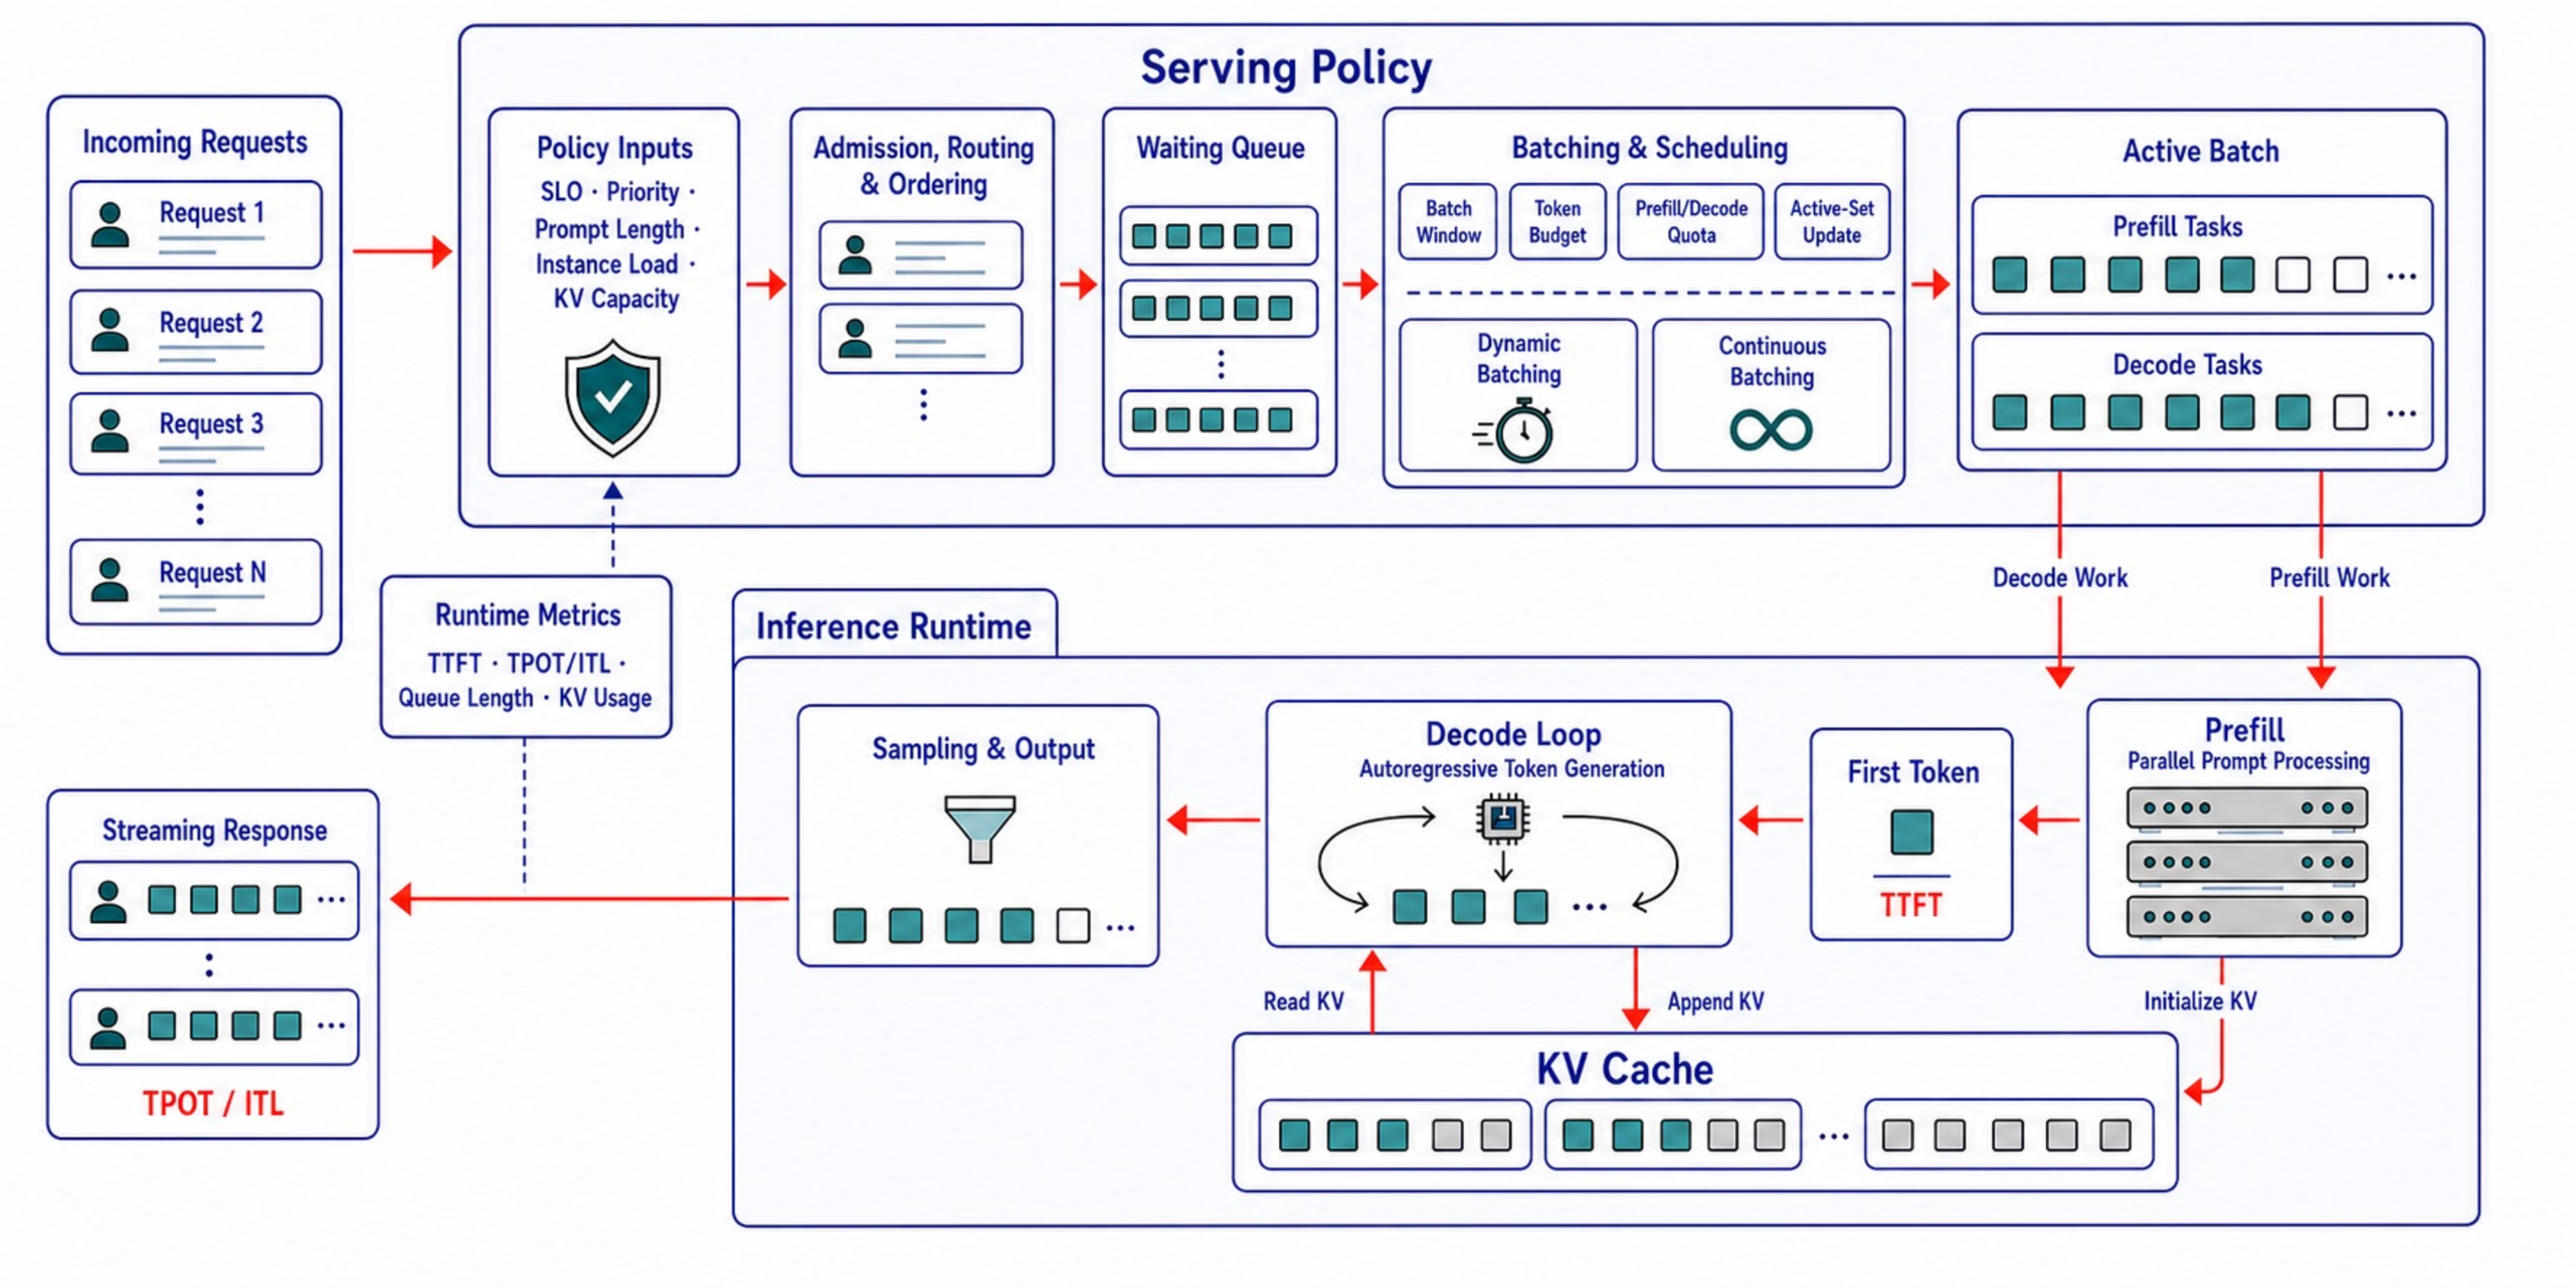
\includegraphics[width=\textwidth]{figures/ch2_llm_serving_workflow.pdf}
    \caption{\textbf{LLM serving 基础服务流程。}Serving policy 作为上层控制面，内部包含准入、路由、排序、请求队列和 batching/scheduling，并根据业务与运行状态形成同时包含 prefill tasks 与 decode tasks 的活动批次；inference runtime 分别执行 Prefill、KV Cache 管理和逐 token Decode，最终形成流式响应并将运行指标反馈给 serving policy。}
    \label{fig:llm-serving-workflow}
\end{figure}

\phantomsection
\subsubsection*{2.1.1 Prefill 与 Decode}
\addcontentsline{toc}{subsubsection}{2.1.1 Prefill 与 Decode}

当今主流的大模型是基于decoder架构的。对于 decoder-only 自回归大模型，一次请求通常分为 \textbf{Prefill} 和 \textbf{Decode} 两个阶段。


\textbf{Prefill 阶段}负责处理完整输入上下文，包括用户 prompt、历史对话、系统提示词和检索增强内容等。模型对整段上下文并行计算 attention 和 FFN，为每一层生成后续 decode 复用的初始 KV Cache，并根据最后位置的输出分布产生首个输出 token。该阶段矩阵规模较大、并行度较高，通常更受计算能力限制，主要影响 TTFT，即 Time To First Token。


\textbf{Decode 阶段}负责逐 token 生成输出。每一步 decode 输入上一步生成的新 token，同时读取历史 KV Cache，计算当前 token 的 attention 和 FFN，并将新增 KV 写回缓存。该阶段每步计算粒度较小、状态依赖强、访存频繁，通常更受显存带宽和单步时延限制，主要影响 TPOT、ITL 和持续生成吞吐。


Prefill 和 Decode 的资源特征差异直接影响 LLM serving 的系统设计。Prefill 以大规模矩阵计算为主，Decode 则由高频、小粒度并且依赖历史状态的迭代组成。因此，推理系统通常分别考虑两个阶段的 batching、调度、KV 管理和分布式执行方式。




\phantomsection
\subsubsection*{2.1.2 KV Cache}
\addcontentsline{toc}{subsubsection}{2.1.2 KV Cache}

KV Cache 是 LLM decode 阶段最核心的运行时状态。自回归生成中，第 t 个 token 的 attention 需要访问前面所有 token 的 key/value。如果每一步都重新计算历史 token 的 key/value，会产生大量重复计算。KV Cache 的作用是在 prefill 阶段保存历史 token 的 key/value，在 decode 阶段复用这些历史 KV，只为新 token 计算新增 KV。


KV Cache 降低了 decode 阶段的重复计算，但也引入了显著的内存状态问题。KV 占用会随 batch size、上下文长度、输出长度、模型层数和 KV head 数增长。在长上下文、多轮对话和高并发场景中，KV Cache 往往成为显存容量和显存带宽的重要瓶颈。vLLM 的 PagedAttention~\cite{kwon2023efficient}、vAttention~\cite{prabhu2025vattention} 的动态 KV 内存管理和 Mooncake~\cite{qin2025mooncake} 的 KVCache-centric serving，分别从分页分配、动态地址映射和分布式 KV 存储等角度降低状态管理开销；相关综述进一步覆盖缓存淘汰、卸载、量化和持久化等方向 \cite{zhou2024survey,pan2025survey}。


典型 KV 相关优化如表~\ref{tab:kv-cache-optimizations} 所示：


\begin{table}[!htbp]
    \centering
    \caption{\textbf{典型 KV Cache 相关优化及作用}}
    \label{tab:kv-cache-optimizations}
    \renewcommand{\arraystretch}{1.45}
    \scriptsize
    \setlength{\tabcolsep}{4pt}
    \begin{tabularx}{\textwidth}{@{}>{\hsize=0.55\hsize\raggedright\arraybackslash}X >{\hsize=1.45\hsize\raggedright\arraybackslash}X@{}}
        \toprule
        \textbf{方向} & \textbf{作用} \\
        \midrule
        PagedAttention / memory paging & 降低 KV 分配碎片，提高显存利用率 \\
        \tabrowrule
        Prefix cache / RadixAttention & 复用共享前缀，减少重复 prefill \\
        \tabrowrule
        KV compression / quantization & 降低 KV 存储和传输成本 \\
        \tabrowrule
        KV eviction & 在显存不足时淘汰低价值 KV \\
        \tabrowrule
        KV offloading & 将部分 KV 放到 CPU、本地存储、远端内存或其他节点 \\
        \tabrowrule
        Distributed KV cache & 在多 worker / 多节点场景下管理 KV 状态分布 \\
        \bottomrule
    \end{tabularx}
\end{table}




\phantomsection
\subsubsection*{2.1.3 Batching 与 Scheduling}
\addcontentsline{toc}{subsubsection}{2.1.3 Batching 与 Scheduling}

Batching 是 LLM serving 提高硬件利用率和吞吐量的主要机制。单个请求在 decode 阶段的每步计算粒度较小，只服务少量请求时加速器容易出现计算单元空闲。Batching 通过合并多个请求扩大矩阵运算规模，提高 GPU/NPU 的并行执行效率，并分摊算子启动和调度等固定开销。


LLM batching 与传统 DNN batching 的执行条件不同。传统推理服务中的动态批处理器通常在请求执行前按等待窗口和 batch size 形成批次 \cite{nvidia2026triton}；LLM 请求的输入长度、到达时间和输出长度差异较大，decode 请求会逐步完成并释放 batch slot，长 prompt 的 prefill 还可能阻塞短请求的 decode。因此，现代 LLM serving 系统通常结合 dynamic batching、continuous batching、iteration-level scheduling 和 chunked prefill。Orca~\cite{yu2022orca} 代表迭代级调度路线，Sarathi-Serve~\cite{agrawal2024taming} 代表 chunked prefill 路线；近期综述也将 batching/scheduling 与算子优化、内存管理并列为 LLM 推理系统的主要组成部分 \cite{zhou2024survey,zhen2025taming,pan2025survey}。


典型调度机制如表~\ref{tab:serving-scheduling-mechanisms} 所示：


\begin{table}[!htbp]
    \centering
    \caption{\textbf{典型 LLM Serving 调度机制及作用}}
    \label{tab:serving-scheduling-mechanisms}
    \renewcommand{\arraystretch}{1.45}
    \scriptsize
    \setlength{\tabcolsep}{4pt}
    \begin{tabularx}{\textwidth}{@{}>{\hsize=0.55\hsize\raggedright\arraybackslash}X >{\hsize=1.45\hsize\raggedright\arraybackslash}X@{}}
        \toprule
        \textbf{机制} & \textbf{作用} \\
        \midrule
        Dynamic batching & 根据请求到达情况动态组成 batch \\
        \tabrowrule
        Continuous batching & 在每个 decode iteration 动态加入新请求、移除完成请求 \\
        \tabrowrule
        Iteration-level scheduling & 以 token iteration 为粒度调度请求 \\
        \tabrowrule
        Chunked prefill & 将长 prompt prefill 拆成多个 chunk，降低对 decode 的阻塞 \\
        \tabrowrule
        Priority / fairness scheduling & 根据 SLA、优先级和公平性调整请求顺序 \\
        \tabrowrule
        Admission control & 在资源紧张时控制进入系统的请求量 \\
        \bottomrule
    \end{tabularx}
\end{table}


Batching 需要根据负载在 throughput、TTFT、TPOT、ITL、显存占用和 SLA 达标率之间动态选择合适的 batch 规模与执行顺序。




\phantomsection
\subsubsection*{2.1.4 主要性能指标}
\addcontentsline{toc}{subsubsection}{2.1.4 主要性能指标}

LLM inference 通常同时关注表~\ref{tab:llm-inference-metrics} 中的指标：


\begin{table}[!htbp]
    \centering
    \caption{\textbf{LLM 推理主要性能指标}}
    \label{tab:llm-inference-metrics}
    \renewcommand{\arraystretch}{1.45}
    \scriptsize
    \setlength{\tabcolsep}{4pt}
    \begin{tabularx}{\textwidth}{@{}>{\hsize=0.55\hsize\raggedright\arraybackslash}X >{\hsize=1.45\hsize\raggedright\arraybackslash}X@{}}
        \toprule
        \textbf{指标} & \textbf{含义} \\
        \midrule
        TTFT & Time To First Token，从请求到达到首个输出 token 返回的时间 \\
        \tabrowrule
        TPOT & Time Per Output Token，首 token 之后每个输出 token 的平均生成时间 \\
        \tabrowrule
        ITL & Inter-token Latency，相邻两个输出 token 的时间间隔，通常同时报告均值和尾部分位数 \\
        \tabrowrule
        E2E latency & 从请求到完整响应结束的端到端时延 \\
        \tabrowrule
        Throughput & 单位时间处理的 request 数或 token 数 \\
        \tabrowrule
        Goodput & 单位时间内满足指定 SLA/SLO 的请求数或 token 数 \\
        \tabrowrule
        GPU/NPU utilization & 加速器计算单元利用率 \\
        \tabrowrule
        Memory footprint & 权重、activation、KV Cache 和运行时空间形成的当前或峰值内存占用 \\
        \tabrowrule
        Cost per token & 单位 token 的计算、显存和服务成本 \\
        \bottomrule
    \end{tabularx}
\end{table}

本文将具体的时延、吞吐和可靠性阈值称为服务目标（SLO），将业务约定的一组服务要求称为 SLA。后文讨论“满足 SLA 的请求处理速度”时，表示只有各项指定 SLO 均达标的请求或运行点才计入结果。




\phantomsection
\subsection*{2.2 LLM 推理的问题空间：从执行机制到系统瓶颈}
\addcontentsline{toc}{subsection}{2.2 LLM 推理的问题空间：从执行机制到系统瓶颈}

LLM 推理的系统瓶颈与其执行机制密切相关。大规模模型参数以及 attention、FFN 计算带来较高的算力和显存开销。Prefill 并行处理完整输入上下文，Decode 则受自回归依赖限制逐 token 生成，两个阶段对计算、显存带宽和时延的要求不同。KV Cache 随上下文长度和并发请求持续增长，又会增加显存容量、访存带宽和状态管理压力。请求到达时间、输入长度和输出长度的变化进一步增加了 batching 与 scheduling 的复杂度；推理扩展到多 GPU、多实例或多节点后，还会引入通信、状态传输和服务编排开销。基于这些问题，本节从五个方面分析主要系统瓶颈。




\phantomsection
\subsubsection*{2.2.1 计算复杂度与模型规模问题}
\addcontentsline{toc}{subsubsection}{2.2.1 计算复杂度与模型规模问题}

模型规模首先决定权重的常驻显存需求和每次前向计算的基本开销；长上下文还会增加 attention 计算与中间状态存储。相关优化需要同时考虑参数表示、模型结构和算子执行效率。

Attention 与 FFN 构成主要矩阵计算，长上下文还会推高 attention 计算和 KV 存储压力。MoE 等条件计算结构可以降低单 token 激活参数量，同时会引入 expert routing、expert placement 和 all-to-all 通信等系统问题。常见优化包括量化、剪枝、蒸馏和低秩分解，以及 GQA/MQA/MLA、高效 attention、MoE 执行优化和低比特算子等方法。




\phantomsection
\subsubsection*{2.2.2 KV Cache 与内存状态问题}
\addcontentsline{toc}{subsubsection}{2.2.2 KV Cache 与内存状态问题}

KV Cache 将 decode 从重复计算历史上下文变为增量计算当前 token，但代价是引入持续增长的运行时状态。上下文越长、batch 越大、并发越高，KV Cache 越容易成为显存容量和带宽瓶颈。

KV Cache 是随请求生命周期动态增长和释放的运行时状态，这使其管理方式不同于静态模型权重。KV Cache 的显存占用会随上下文长度和并发度增长，动态分配释放又容易产生碎片；在多轮对话和共享 prompt 场景中，不同请求可能重复执行相同前缀的 prefill；在跨 worker 或跨节点 serving 中，KV 的传输、迁移、复用和远程访问会进入端到端时延关键路径。PagedAttention、prefix cache、KV compression、KV quantization、KV eviction、KV offloading、distributed KV cache 和 remote KV serving 等方法，分别用于降低状态成本、提高状态复用或控制状态移动。




\phantomsection
\subsubsection*{2.2.3 请求动态性与调度问题}
\addcontentsline{toc}{subsubsection}{2.2.3 请求动态性与调度问题}

LLM 请求具有高度动态性：prompt 长度不同、输出长度未知、请求到达时间随机、服务质量目标不同。Prefill 和 decode 的资源特征也不同，长 prefill 可能阻塞短 decode，请求完成时间差异又会导致 batch 内部动态变化。

调度问题的核心是吞吐和时延之间的动态权衡。等待凑 batch 可以提高硬件利用率，但会增加 TTFT；过大的 batch 会推高单请求延迟和显存占用；长 prompt prefill 可能阻塞已经进入流式输出的 decode 请求；不同租户、优先级和 SLA 又会使简单 FIFO 策略失效。因此，现代 LLM serving 通常采用 dynamic batching、continuous batching、iteration-level scheduling、chunked prefill、deadline-aware scheduling、priority scheduling 和 admission control 等机制，在 batch 形成、active set 更新和请求优先级之间做在线决策。




\phantomsection
\subsubsection*{2.2.4 Decode 串行性与生成加速问题}
\addcontentsline{toc}{subsubsection}{2.2.4 Decode 串行性与生成加速问题}

LLM decode 是自回归过程，每一步依赖前一步输出，天然存在串行依赖。即使单步 forward 被加速，逐 token 生成仍可能造成较高 TPOT 和 ITL。

这一串行依赖存在于不同规模的自回归模型中，但单步开销仍会随模型规模、上下文长度和 batch 状态变化。单步 decode 的计算粒度较小，硬件利用率往往不如 prefill；sampling、beam search 或复杂生成策略还会增加控制开销。Speculative decoding、assisted decoding、parallel decoding、tree decoding 和 multi-token prediction 等方法，试图通过草稿生成、批量验证或一次预测多个 token 来减少目标模型的串行调用次数，但仍需权衡草稿接受率、额外计算、输出质量和系统复杂度。




\phantomsection
\subsubsection*{2.2.5 多实例、多 GPU 与服务级编排问题}
\addcontentsline{toc}{subsubsection}{2.2.5 多实例、多 GPU 与服务级编排问题}

当模型规模、并发量或服务可用性需求超过单设备能力时，系统需要跨多个 GPU、worker、replica 或节点协同。此时问题从单个 engine 内部执行扩展为分布式执行和服务级调度。

分布式化带来的收益与代价同时存在。Tensor、pipeline、expert 或 context parallel 可以突破单设备容量和吞吐限制，但会引入 activation、KV 和中间状态的跨设备传输；prefill 与 decode 的资源特征差异使 disaggregation 成为可能，也使 KV handoff 成为新的关键路径；多 replica 和多模型服务可以提高可用性和弹性，却需要在负载均衡、质量、时延和成本之间做服务级选择。因此，distributed parallelism、prefill/decode disaggregation、distributed KV cache、KV transfer、replica routing、cluster load balancing、cascade serving 和 speculative serving orchestration 等方法，本质上都在处理“如何把单实例推理扩展成可控的分布式服务”这一问题。




\phantomsection
\subsection*{2.3 LLM 推理优化的“优化对象--执行范围”分类}
\addcontentsline{toc}{subsection}{2.3 LLM 推理优化的“优化对象--执行范围”分类}

围绕 LLM inference 相关优化方向分类的 overview 和 survey 工作较多，表~\ref{tab:existing-inference-taxonomies} 汇总了其中代表性工作的分类方式及其特点。

\begin{table}[!htbp]
    \centering
    \caption{\textbf{现有 LLM Inference Overview 与 Survey 的分类方式}}
    \label{tab:existing-inference-taxonomies}
    \renewcommand{\arraystretch}{1.4}
    \scriptsize
    \setlength{\tabcolsep}{4pt}
    \begin{tabularx}{\textwidth}{@{}>{\hsize=0.95\hsize\raggedright\arraybackslash}X >{\hsize=0.65\hsize\raggedright\arraybackslash}X >{\hsize=1.25\hsize\raggedright\arraybackslash}X >{\hsize=1.15\hsize\raggedright\arraybackslash}X@{}}
        \toprule
        \textbf{工作} & \textbf{分类视角} & \textbf{主要分类} & \textbf{分类特点} \\
        \midrule
        \textit{A Survey on Efficient Inference for Large Language Models} \cite{zhou2024survey}
        & 优化层次
        & Data-Level、Model-Level、System-Level
        & 覆盖从输入数据、模型结构到系统实现的多层优化，适合从整体上理解推理效率优化 \\
        \tabrowrule
        \textit{A Survey of LLM Inference Systems} \cite{pan2025survey}
        & 系统流水线与系统形态
        & Request processing、model optimization and execution、memory management，以及 single-replica、multi-replica、disaggregated、serverless systems
        & 对 system-level 方法拆分较细，突出 kernel、batching/scheduling、memory management 与不同部署形态 \\
        \tabrowrule
        \textit{Taming the Titans: A Survey of Efficient LLM Inference Serving} \cite{zhen2025taming}
        & Serving 层级与场景
        & Instance-Level Approaches、Cluster-Level Strategies、Emerging Scenarios、Miscellaneous Areas
        & 强调从单实例优化扩展到集群部署、负载均衡和云服务等 serving 问题 \\
        \bottomrule
    \end{tabularx}
\end{table}

基于这些工作，本报告采用“优化对象--执行范围”二维分类。第一维按照方法直接改变的对象，将其分为 Model、Kernel、Runtime 和 Serving Policy \& Routing 四层；第二维按照执行范围，区分单实例或本地控制域内的 Local 优化，以及需要跨设备、worker、replica 或节点协同的 Distributed 优化。图~\ref{fig:layer-scope-taxonomy} 展示了两条分类轴，后续 2.3.1--2.3.4 分别说明四类优化对象及其本地和分布式实现。

\begin{figure}[H]
    \centering
    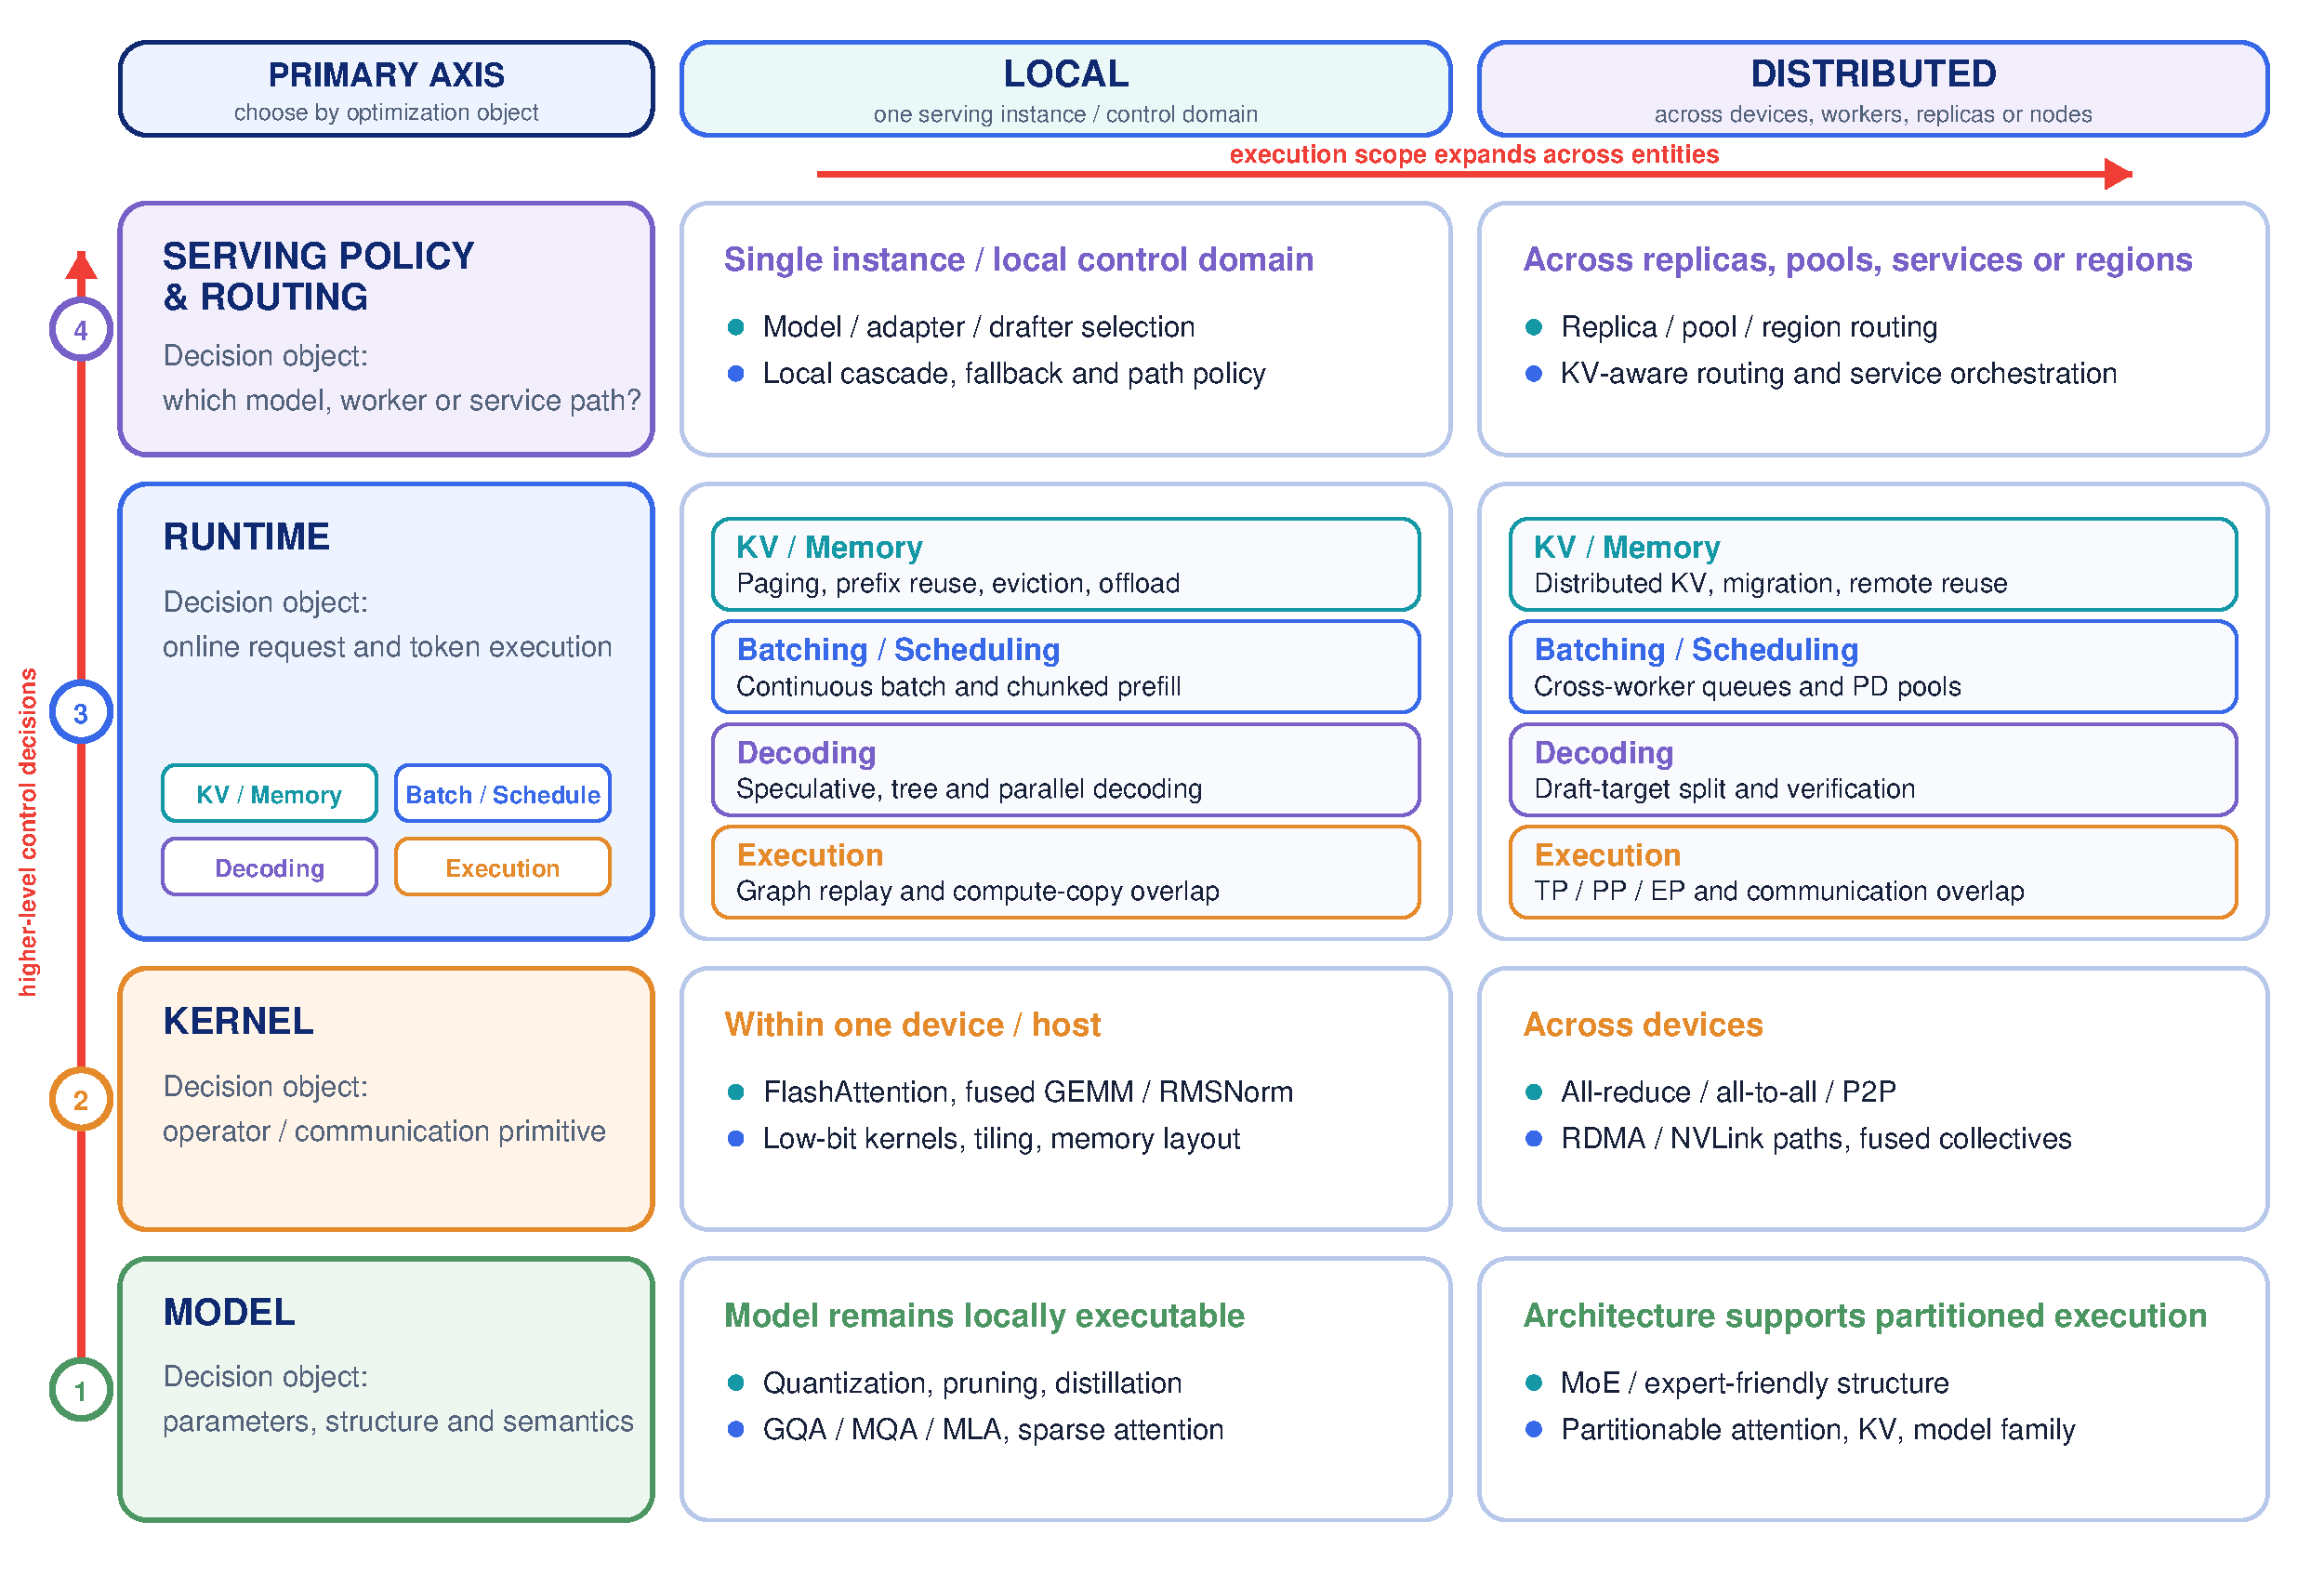
\includegraphics[width=\textwidth]{figures/ch2_layer_scope_taxonomy.pdf}
    \caption{\textbf{LLM 推理优化的“优化对象--执行范围”二维分类。}纵轴按照主要优化对象区分 Model、Kernel、Runtime 与 Serving Policy \& Routing 四个层级；横轴按照执行范围区分 Local 与 Distributed，表示方法从单实例或本地控制域扩展到跨设备、worker、replica、service 或 node 的协同。Runtime 层进一步包含 KV/Memory、Batching/Scheduling、Decoding 和 Execution 四类在线机制。}
    \label{fig:layer-scope-taxonomy}
\end{figure}

其中，Local 表示优化限制在单个 serving instance 或本地控制域内，可以包含 CPU 与 GPU/NPU、本地内存和存储之间的协同；Distributed 表示方法需要跨多个设备、worker、replica 或节点分配计算、请求、KV 状态或 activation。四类方法并不互斥，真实系统经常同时使用多层机制。因此，归类时主要判断三个问题：方法解决什么问题，直接改变的对象是什么，以及是否需要跨设备或跨节点协同。




\phantomsection
\subsubsection*{2.3.1 Model-Level Optimization}
\addcontentsline{toc}{subsubsection}{2.3.1 Model-Level Optimization}

Model-Level Optimization 直接改变模型参数、参数表示、结构设计或算法语义，以降低推理计算和存储开销。此类修改不依赖某个特定 serving engine，其优化对象包括参数量、权重表示、FLOPs、activation 计算量、attention 复杂度、KV 大小以及条件计算路径。

\textbf{Local scope：}常见方法包括权重量化、剪枝、蒸馏、低秩分解、权重共享、GQA/MQA/MLA、线性或稀疏 attention、状态空间模型、early exit、token pruning 和动态稀疏等，主要用于单实例或单设备上的模型压缩和结构简化。

\textbf{Distributed scope：}主要关注模型结构对跨设备执行的支持，例如适合 expert parallelism 的 MoE 结构、适合 tensor/context parallel 的 attention 或 KV 结构，以及便于按 layer、expert、context 或 activation 切分的模型设计。

CUDA Graph、算子融合和 TensorRT execution graph 等方法主要改变执行路径或部署图，分别归入 Runtime-Level 或 Kernel-Level；它们不会改变模型参数和数学语义。




\phantomsection
\subsubsection*{2.3.2 Kernel-Level Optimization}
\addcontentsline{toc}{subsubsection}{2.3.2 Kernel-Level Optimization}

Kernel-Level Optimization 在保持模型数学语义不变的条件下，优化张量算子或通信原语在硬件上的执行效率。主要对象包括 attention、GEMM、normalization、sampling 和 collective communication，目标是提高 GPU/NPU 利用率、减少 HBM 访问、增强片上缓存复用，并改善算子吞吐。

\textbf{Local scope：}典型方法包括 FlashAttention、FlashDecoding 和 paged attention kernel。其他方法还包括 MLP、RMSNorm 与 softmax 融合，低比特 GEMM，FP8、INT8 与 INT4 算子，硬件感知 tiling、内存布局优化和 GPU-side sampling。

\textbf{Distributed scope：}主要包括集合通信和点对点通信原语的实现优化，例如 all-reduce、all-gather、reduce-scatter、all-to-all、RDMA/NVLink 传输路径、通信融合、集合通信算法选择，以及 MoE expert dispatch/combine 原语。

需要区分的是，如果优化对象是 collective / P2P primitive 的实现路径，归为 Kernel-Level × Distributed；如果优化对象是通信与计算在 runtime pipeline 中的编排、重叠和调度，则归为 Runtime-Level × Distributed。




\phantomsection
\subsubsection*{2.3.3 Runtime-Level Optimization}
\addcontentsline{toc}{subsubsection}{2.3.3 Runtime-Level Optimization}

Runtime-Level Optimization 是现代 LLM serving 的主要系统优化层。它发生在请求进入 inference engine 之后，管理在线 token 执行、KV 状态、batch 组成、decode 循环和执行流水线。Runtime-Level 不改变模型语义，也不一定修改单个 kernel，而是决定请求到达后如何组织执行。本文将其进一步分为 KV / Memory、Batching / Scheduling、Decoding 和 Execution 四类运行时机制。

\begin{enumerate}
    \item \textbf{KV / Memory Runtime.} KV / Memory Runtime 关注 KV lifecycle、memory state 和 cache reuse。它的核心问题是：KV Cache 如何存储、复用、压缩、淘汰、迁移或远程访问。

    \textbf{Local scope：}主要包括 KV cache management、PagedAttention / memory paging、Prefix cache / RadixAttention、KV compression / quantization、KV eviction、KV offloading、cache persistence 和 runtime memory allocator 等机制。

    \textbf{Distributed scope：}问题进一步扩展为 distributed KV cache、KV transfer / migration、remote KV serving、multi-replica KV reuse、distributed prefix cache、KV-aware placement 和 cross-worker state synchronization。

    这一类优化的核心目标是降低 KV 显存占用、减少重复 prefill、提升 cache reuse，并在分布式场景下控制 KV 传输和状态迁移成本。

    \item \textbf{Batching / Scheduling Runtime.} Batching / Scheduling Runtime 关注请求和 token 在 inference engine 内如何组织执行。它回答的是：哪些请求何时执行，哪些 token 可以组成 batch，prefill 和 decode 如何交错，如何在 throughput、TTFT、TPOT、ITL、公平性和 SLA 之间做权衡。

    \textbf{Local scope：}典型机制包括 dynamic batching、continuous batching、iteration-level scheduling、chunked prefill、prefill/decode interleaving、engine-local admission control、priority / fair scheduling 和 deadline-aware scheduling。

    \textbf{Distributed scope：}调度对象会跨越 worker、replica 或资源池，因此需要 cross-worker scheduling、distributed continuous batching、prefill worker / decode worker scheduling、heterogeneous GPU scheduling、multi-replica queue coordination、distributed admission control 和 SLO-aware worker scheduling。

    这一类优化的核心目标是在动态请求负载下提高硬件利用率，同时控制排队时延和服务质量。

    \item \textbf{Decoding Runtime.} Decoding Runtime 关注在线 token generation procedure。它回答的是：输出 token 如何生成、验证、选择和接受。它不主要决定请求如何组 batch，也不主要决定计算如何 launch，而是改变 decode loop 的生成逻辑。

    \textbf{Local scope：}这类方法包括 speculative decoding、assisted decoding、parallel decoding、tree decoding、beam search optimization、n-gram speculation、prompt lookup decoding 和 serving-time multi-token prediction / verification。

    \textbf{Distributed scope：}Decoding Runtime 会涉及 distributed verification、draft / target execution split、multi-draft execution、batched verification across workers、draft model 与 target model 分布式协同，以及 speculative decoding 与 prefill/decode disaggregation 的结合。

    Speculative decoding 有时也被称为 decoding algorithm。本文将其主要归入 Runtime-Level，因为它改变的是服务阶段的 token 生成与验证过程，而不是原模型参数或主体结构。如果某种 multi-token prediction 方法新增训练 head 或修改模型结构，则还应同时标注其 Model-Level 属性。

    \item \textbf{Execution Runtime.} Execution Runtime 关注已经排定的计算如何提交、同步、重放和重叠执行。当前面的运行时已经决定请求集合、batch 组成和 decode 方式后，Execution Runtime 负责把算子、数据搬运和通信提交到硬件，并组织为流水线。

    \textbf{Local scope：}主要包括 CUDA Graph / HIP Graph replay、async execution、stream scheduling、CPU-GPU overlap、host-device communication hiding、compute / memory-copy overlap、runtime metadata / buffer reuse 和 GPU-side sampling execution path。

    \textbf{Distributed scope：}主要包括 tensor parallel runtime、pipeline parallel runtime、expert parallel runtime、context / sequence parallel runtime、prefill/decode disaggregation、distributed execution pipeline、communication-computation overlap scheduling 以及 activation / KV transfer orchestration。

    Execution Runtime 与 Kernel-Level 的边界在于：Kernel-Level 优化单个 operator 或 communication primitive 的实现；Execution Runtime 优化一组 operator、copy 和 communication 的 launch、同步、overlap 和流水化组织方式。
\end{enumerate}

\phantomsection
\subsubsection*{2.3.4 Serving Policy \& Routing-Level Optimization}
\addcontentsline{toc}{subsubsection}{2.3.4 Serving Policy \& Routing-Level Optimization}

Serving Policy \& Routing-Level Optimization 关注服务级控制决策。它不直接决定单个 engine 内部的 token 如何执行，而是选择请求使用哪个模型、adapter、replica、worker pool 或服务路径，并处理回退、级联和多服务编排。典型决策包括请求分配、模型或 adapter 选择、实例选择、服务路径选择，以及面向 SLO、成本和时延的路由策略。

\textbf{Local scope：}主要包括 local model selection、adapter / LoRA routing、local cascade serving、normal decoding 与 speculative decoding path selection、drafter selection、local/cloud fallback、budget-aware local inference 和 latency-aware local policy。

\textbf{Distributed scope：}进一步扩展为 replica routing、worker-pool routing、cluster load balancing、SLO-aware routing、cost-aware routing、region-aware routing、KV-aware routing、speculative serving orchestration、draft-target worker orchestration 和 multi-service graph orchestration。

Runtime-Level 和 Serving Policy \& Routing-Level 在真实系统中相互依赖，但主要决策对象不同。前者解决“请求进入某个 engine 后如何执行”，后者解决“请求交给哪个模型、worker、replica 或服务路径”。服务级决策通常需要读取队列长度、KV Cache 压力、batch 状态和请求距离 SLO 阈值的剩余时间。




\phantomsection
\subsection*{2.4 主流 LLM 推理框架及优化方式}
\addcontentsline{toc}{subsection}{2.4 主流 LLM 推理框架及优化方式}

LLM 推理框架把模型加载、算子执行、KV Cache 管理、请求调度和服务接口组合成可部署的推理系统。vLLM 以 PagedAttention 和 continuous batching 为基础，重点提高通用 GPU 服务器上的显存利用率与在线服务吞吐；TensorRT-LLM 面向 NVIDIA GPU，通过专用 kernel、低精度计算、in-flight batching 和多 GPU 并行提供高度优化的执行路径；SGLang 从结构化生成程序出发，将 RadixAttention、请求调度和分布式执行整合到同一运行时；LMDeploy/TurboMind 面向开源模型部署，提供模型转换与量化、persistent batching、blocked KV Cache 和多 GPU 执行等能力 \cite{kwon2023efficient,nvidia2026tensorrt,zheng2024sglang,lmdeploy2026documentation}。表~\ref{tab:framework-mechanism-mapping} 按主要优化对象和执行范围汇总这些框架的代表性机制；该表不覆盖各框架的全部功能。


\begin{table}[H]
    \centering
    \caption{\textbf{主流 LLM Inference Framework 代表性机制映射}}
    \label{tab:framework-mechanism-mapping}
    \renewcommand{\arraystretch}{1.45}
    \scriptsize
    \setlength{\tabcolsep}{4pt}
    \begin{tabularx}{\textwidth}{@{}>{\hsize=0.75\hsize\raggedright\arraybackslash}X >{\hsize=0.75\hsize\raggedright\arraybackslash}X >{\hsize=1.15\hsize\raggedright\arraybackslash}X >{\hsize=1.15\hsize\raggedright\arraybackslash}X >{\hsize=1.20\hsize\raggedright\arraybackslash}X@{}}
        \toprule
        \textbf{Framework} & \textbf{代表性方法 / 机制} & \textbf{解决的具体问题} & \textbf{优化方向分类层 \& Scope} & \textbf{具体方法说明} \\
        \midrule
        \frameworkcell{\textbf{vLLM}~\cite{kwon2023efficient}} & PagedAttention & KV Cache 动态分配和显存碎片问题 & Runtime / KV-Memory × Local & 通过分页式 KV 管理降低显存碎片，提高 KV Cache 利用率 \\
        \cmidrule(l){2-5}
         & Continuous batching & Decode 阶段请求动态进出，静态 batch 利用率低 & Runtime / Batching-Scheduling × Local & 在 decode iteration 动态加入和移除请求，提高高并发吞吐 \\
        \cmidrule(l){2-5}
         & Chunked prefill & 长 prompt prefill 阻塞 decode，影响 TTFT / ITL & Runtime / Batching-Scheduling × Local & 将长 prefill 拆分为 chunk，与 decode 交错执行 \\
        \cmidrule(l){2-5}
         & Prefix caching & 多请求共享前缀导致重复 prefill & Runtime / KV-Memory × Local/Distributed & 复用共享 prompt 或 prefix，减少重复 prefill 计算 \\
        \tabrowrule
        \frameworkcell{\textbf{TensorRT-LLM}~\cite{nvidia2026tensorrt}} & In-flight batching & 高并发请求长度不同，传统 batching 效率低 & Runtime / Batching-Scheduling × Local & 对不同阶段和长度的请求进行动态批处理 \\
        \cmidrule(l){2-5}
         & Paged KV Cache & KV Cache 分配、复用和显存管理问题 & Runtime / KV-Memory × Local & 通过 paged KV 管理改善 KV Cache 利用率 \\
        \cmidrule(l){2-5}
         & FP8 / INT8 / INT4 execution & 权重、activation 和算子执行成本高 & Model + Kernel × Local/Distributed & 通过低比特模型表示和低比特 kernel 降低显存和计算成本 \\
        \cmidrule(l){2-5}
         & Overlap scheduler & compute、copy、communication、prefill/decode 没有充分重叠 & Runtime / Execution × Local/Distributed & 将计算、通信和数据搬运流水线化，减少等待 \\
        \tabrowrule
        \frameworkcell{\textbf{SGLang}~\cite{zheng2024sglang}} & RadixAttention & 多轮、多分支请求存在大量共享前缀 & Runtime / KV-Memory × Local & 用 radix tree 组织 prefix cache，提高共享前缀复用 \\
        \cmidrule(l){2-5}
         & Zero-overhead CPU scheduler & 高并发场景下 CPU 调度开销影响吞吐 & Runtime / Batching-Scheduling × Local & 降低 CPU 侧调度和 metadata 管理开销 \\
        \cmidrule(l){2-5}
         & Prefill-decode disaggregation & Prefill 和 decode 资源特征不同，混部互相干扰 & Runtime / Execution × Distributed & 将 prefill 与 decode 分离到不同资源池，减少资源干扰 \\
        \cmidrule(l){2-5}
         & Multi-LoRA batching & 多 adapter 请求混合服务时 batch composition 复杂、吞吐下降 & Serving Policy \& Routing + Runtime/Scheduling × Local/Distributed & 将不同 LoRA / adapter 请求合并调度，提高多 LoRA serving 效率 \\
        \tabrowrule
        \frameworkcell{\textbf{Hugging Face TGI}~\cite{huggingface2026tgi}} & Continuous batching & incoming requests 动态变化，传统 batching 吞吐不足 & Runtime / Batching-Scheduling × Local & 动态合并请求，提高在线 serving 吞吐 \\
        \cmidrule(l){2-5}
         & Flash Attention & attention HBM traffic 高，operator throughput 受限 & Kernel × Local & 通过高效 attention kernel 降低显存访问并提升算子吞吐 \\
        \cmidrule(l){2-5}
         & Paged Attention & KV Cache / attention memory 管理效率不足 & Runtime / KV-Memory × Local & 通过 paged attention 改善 attention/KV memory 管理 \\
        \cmidrule(l){2-5}
         & Tensor parallelism & 单 GPU 容量或吞吐不足，需要跨 GPU 执行 & Runtime / Execution × Distributed & 将模型执行切分到多个 GPU，提高模型容量和吞吐 \\
        \tabrowrule
        \frameworkcell{\textbf{LMDeploy / TurboMind}~\cite{lmdeploy2026documentation}} & Persistent batching & 高并发请求动态调度，提高吞吐 & Runtime / Batching-Scheduling × Local & 通过持续批处理机制维持 batch 执行效率 \\
        \cmidrule(l){2-5}
         & Blocked KV Cache & KV Cache 显存管理和访问效率问题 & Runtime / KV-Memory × Local & 通过 block-based KV 管理改善显存利用率 \\
        \cmidrule(l){2-5}
         & Dynamic split \& fuse & 长 prompt 和 decode 混合执行效率低 & Runtime / Batching-Scheduling × Local & 动态拆分和融合 prefill / decode 任务，提高混合负载效率 \\
        \cmidrule(l){2-5}
         & Tensor parallelism & 大模型需要跨 GPU 执行 & Runtime / Execution × Distributed & 支持模型在多 GPU 上并行执行 \\
        \bottomrule
    \end{tabularx}
\end{table}

从主要部署对象看，上述框架目前仍以数据中心或服务器场景为主。其核心能力围绕单机多 GPU、多机多 GPU、高并发请求、稳定高速互联和统一加速器软件栈展开。具有兼容 GPU 或 NPU 的边缘服务器可以复用其中部分执行引擎，但这些框架本身通常不负责处理移动终端的功耗限制、端侧内存约束、间歇性链路、跨边缘节点状态放置和用户移动等问题。

边缘侧较有代表性的 LLM 推理框架包括 llama.cpp~\cite{llamacpp2026documentation} 和 MLC LLM~\cite{mlcllm2026documentation}。llama.cpp 使用轻量 C/C++ 运行时和 GGUF 模型格式，支持多种低比特量化、CPU/GPU 混合执行以及 Android 和 Apple 平台；MLC LLM 通过机器学习编译生成面向不同硬件后端的模型库，并以同一引擎支持 Web、iOS、Android、Python 和 REST 部署。这类框架的重点是让量化后的模型在单台手机、PC 或嵌入式设备上运行，其请求并发、跨节点 KV Cache 管理和全局调度能力仍弱于数据中心推理框架。

除单设备运行时外，已有部分研究围绕模型切分、异构资源调度和跨节点通信等问题，对多节点协同推理开展了方法设计与实验探索。总体来看，边缘侧单设备推理已具备较为成熟的软件实现，而多节点协同推理仍以面向特定问题的研究方案为主，尚未形成能够统一处理资源变化、链路波动、推理状态管理和用户移动的动态 CEC 服务框架。




\phantomsection
\subsection*{2.5 小结}
\addcontentsline{toc}{subsection}{2.5 小结}

本章首先介绍了 LLM inference 的基本执行机制，包括 prefill/decode、KV Cache、batching/scheduling 和主要性能指标。随后，从执行机制出发，总结了 LLM inference 的主要问题空间，包括计算复杂度与模型规模、KV Cache 与内存状态、请求动态性与调度、decode 串行性与生成加速，以及多实例、多 GPU 与服务级编排问题。


在已有 overview 和 survey 工作的基础上，本章采用“优化对象--执行范围”二维分类：按照方法直接改变的对象区分 Model、Kernel、Runtime、Serving Policy \& Routing，并按照是否跨设备或节点区分 Local 与 Distributed。Runtime 层进一步细分为 KV / Memory、Batching / Scheduling、Decoding 和 Execution 四类机制。该分类可同时说明一个方法改动了什么，以及它在单实例内执行还是需要分布式协同。


最后，本章通过主流推理框架的代表性机制映射说明，实际系统通常会组合模型表示、kernel、KV 管理、batching/scheduling、执行运行时和服务策略等多层机制。现有通用服务框架主要面向数据中心，边缘侧单设备运行时已经具备工程可用性，而多节点协同服务仍以研究原型为主。该分类框架将用于后续分析 CEC 场景下的模型部署、请求调度、KV 状态迁移和服务路径选择。

\phantomsection
\section*{三、CEC 场景下的大模型推理}
\addcontentsline{toc}{section}{三、CEC 场景下的大模型推理}

\phantomsection
\subsection*{3.1 CEC LLM 推理的系统形态}
\addcontentsline{toc}{subsection}{3.1 CEC LLM 推理的系统形态}

CEC 场景下的大模型推理运行在由多个地理分布、能力异构的边缘节点组成的协作系统中 \cite{duan2022distributed}。协作节点可以是具备推理能力的终端设备、边缘服务器和 AI 板卡，也可以是部署在基站、网关或园区中的推理实例；请求可从终端、基站或边缘网关等任一入口进入。模型权重、adapter（参数高效微调模块）、KV Cache、prefix cache、session state 和中间状态可以集中在单个节点，也可以分布在多个协作节点上。一次推理既可以在本地实例内完成，也可以通过节点间的计算与状态传输协同完成；外部云服务仅在具体业务允许时作为可选服务或回退路径。

与云侧集中式 LLM serving 相比，CEC 的主要变化是执行范围从单个实例或集中式集群扩展到分布式边缘资源池。云侧 serving 通常具有相对集中的资源和稳定互联，优化重点是单实例或集群内部的吞吐、显存和调度效率。CEC 还需要把节点位置、无线与边缘网络、异构硬件、移动接入、状态分布和隐私边界纳入推理路径。推理系统需要同时确定执行实例、跨节点模型部署、状态保留位置、节点间传输方式和服务路径调整条件。图~\ref{fig:cec-llm-serving-architecture} 展示了模型分割部署、计算任务调度和 KV/runtime state 调度在协作边缘节点之间的关系。

\begin{figure}[!htbp]
    \centering
    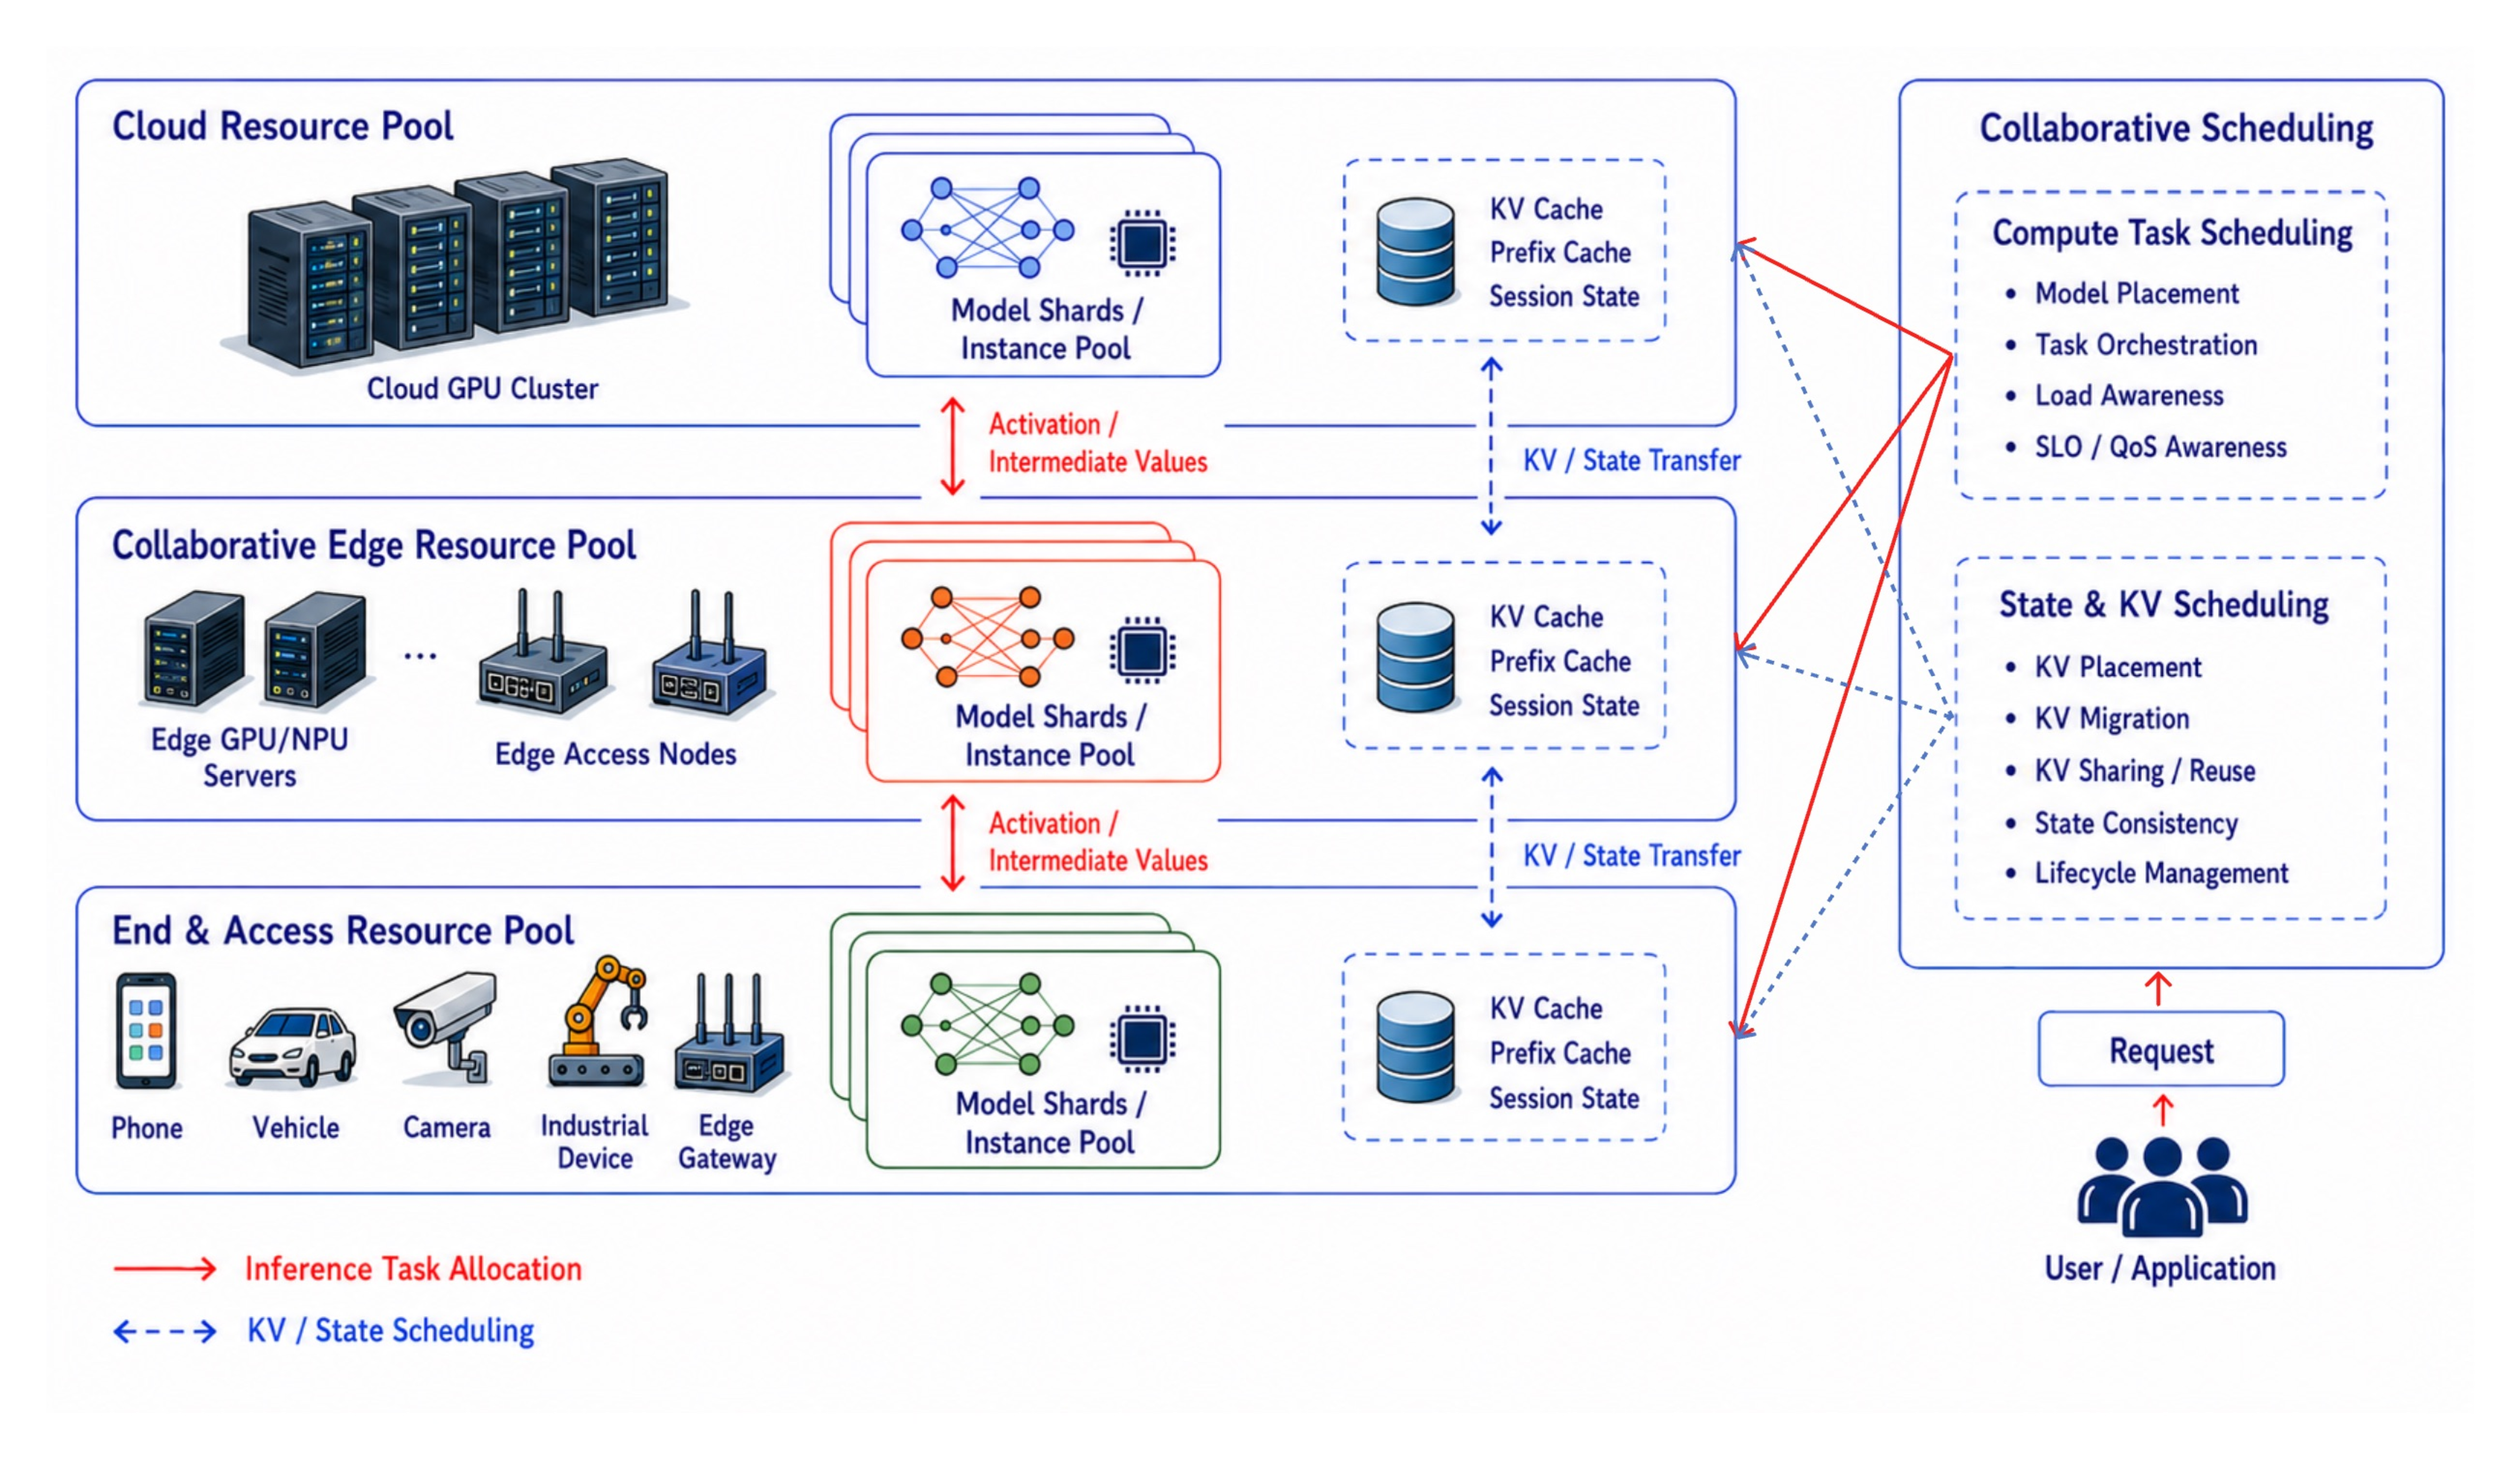
\includegraphics[width=\textwidth]{figures/ch3_cec_llm_serving_architecture.pdf}
    \caption{\textbf{CEC 环境下的 LLM 推理 Serving 系统形态。}Serving Policy 根据协作节点的资源、链路与运行状态，协调模型分割与部署、Prefill/Decode 等计算任务调度，以及 KV Cache、Prefix Cache 和 Session State 的复用、迁移与远程访问。}
    \label{fig:cec-llm-serving-architecture}
\end{figure}

CEC LLM inference 主要包含三类相互关联的决策。模型部署决定模型的哪些部分由哪些协作节点执行；实例内调度决定请求如何组成 batch，以及 prefill 和 decode 如何安排；服务路径选择决定请求、会话和运行时状态在协作节点之间如何路由、迁移或复用。后续章节分别围绕这三类问题展开。

\phantomsection
\subsection*{3.2 CEC 相较云侧集中式 LLM Serving 新增的约束}
\addcontentsline{toc}{subsection}{3.2 CEC 相较云侧集中式 LLM Serving 新增的约束}

\textbf{资源受限与硬件异构：}模型规模、KV Cache、batching、并行执行和多实例调度在云侧同样存在，CEC 则进一步面临单节点资源受限和设备能力差异。协作资源池中的终端设备、边缘服务器和 AI 板卡在算力、显存、内存、功耗及散热预算上差异明显，同一个模型未必能完整放入目标设备；即便容量足够，也可能受到低比特算子、算子覆盖范围、推理后端和数据布局转换的限制。因此，部署方案必须同时考虑设备容量、实际执行能力和节点间通信。

\textbf{网络波动与状态移动成本：}终端接入链路和边缘节点间链路的带宽、RTT、抖动与拥塞状态会直接影响模型切分、task offloading、prefill/decode 分离和 KV 迁移是否值得执行。对于普通 DNN 推理，跨节点传输的主要对象通常是输入或中间 activation；而在 LLM inference 中，KV Cache、prefix cache、session state 和多轮上下文也会成为需要迁移或远程访问的状态资源。网络成本因此不再只是请求入口到服务实例的传输延迟，而是贯穿推理全过程的状态移动成本。

\textbf{请求负载突发且SLO要求异构：}单个请求入口附近的边缘节点通常资源受限，请求到达具有突发性，并且不同请求的SLO要求各不相同。等待较大的 batch 会增加 TTFT，完全放弃 batching 又会降低 GPU/NPU 利用率。prefill 与 decode 的资源需求不同，长短请求和不同 SLA 请求混合到达时，固定 batch size 与 FIFO 队列很难同时保证吞吐和尾时延。因此，边缘运行时需要根据当前队列、请求时限、KV 占用和阶段负载动态调整组批与执行顺序，以满足不同请求的SLO要求。

\textbf{用户移动与服务连续性：}对于单轮短请求，移动可能只改变入口节点；对于多轮对话、长上下文和 agent workflow，移动会改变服务实例与状态位置之间的关系。KV Cache、prefix cache、session state 或 agent memory 可能仍然停留在原服务节点，新请求却已经从新的入口进入系统。系统需要在迁移状态、远程访问原有状态、重新 prefill 或缩短可用上下文之间做选择。因此，评价指标还需要覆盖会话连续性、状态复用和移动场景下的 QoS 稳定性。

\textbf{隐私边界与数据本地性：}部分 prompt、传感器数据、业务上下文或用户状态可能不能离开本地边缘域，也可能只允许在指定节点集合内流动。隐私约束会限制模型选择、offloading 范围、KV 迁移路径和 fallback 策略，使系统不能仅按最小时延或最低成本选择节点。换言之，CEC 中的推理优化必须同时处理资源可行性、链路代价、状态位置、隐私边界和业务 QoS。

\phantomsection
\subsection*{3.3 现有 LLM Inference 优化在 CEC 中的关注重点}
\addcontentsline{toc}{subsection}{3.3 各类 LLM Inference 优化在 CEC 中的关注重点}

\textbf{Model-Level：关注模型表示与结构能否适配目标设备。}量化、剪枝和小模型替代会改变模型的容量与计算需求，GQA、MoE 等结构还会影响 KV 大小、条件计算和通信模式。模型结构是否便于按 layer、tensor 或 expert 拆分，会影响跨节点部署的可行性；具体分割位置、并行度和执行顺序则由分布式 Runtime 决定。

\textbf{Kernel-Level：关注异构硬件的算子支持与执行效率。}CEC 系统可能同时包含不同规格的 NPU、GPU、CPU 及 AI 板卡。各后端支持的数据精度、算子、attention kernel、KV 布局和通信原语并不一致。一个模型在数据中心 GPU 上能够高效执行，并不意味着它在边缘设备上具有相同性能；不受支持的算子、数据布局转换和 CPU 回退都可能抵消协同执行的收益。

\textbf{Runtime-Level：把网络和状态纳入在线执行控制。}云侧 runtime 主要管理单个 serving engine 或集中式集群内的 KV、batch 和执行流水线；CEC runtime 还要读取链路状态、节点负载、KV 位置和用户入口变化。KV 管理由单实例显存分配扩展为跨节点状态管理，batching 需要适应SLO要求异构且动态的请求池，分布式执行则要同时安排节点计算和跨节点数据传输。

\textbf{Serving Policy \& Routing-Level：联合选择执行节点和状态处理方式。}一个请求是在入口节点执行，还是交给其他协作节点，需要同时考虑模型可用性、链路状态、节点负载、KV/cache 位置、用户入口变化、隐私限制和 SLA 风险。除选择执行节点外，服务策略还要决定状态是本地复用、跨节点同步、远程访问还是重新计算。

在 CEC 中，模型部署、运行时调度和服务路径选择共享同一组设备、链路和状态条件。模型切分决定执行拓扑和通信量，batching 改变实例容量与排队时间，KV 状态位置又会影响请求卸载代价。基于这种关系，后续章节按模型切分、业务感知 batching 和请求卸载三类具体问题组织相关工作与方案。

\phantomsection
\subsection*{3.4 本文采用的 CEC LLM Inference 综述框架}
\addcontentsline{toc}{subsection}{3.4 本文采用的 CEC LLM Inference 综述框架}

基于上述分析，本文将 CEC 场景下的 LLM inference 优化归纳为三条主线。第一条是资源自适应模型部署，对应模型计算如何分配到协作节点。第 4 章的相关工作综述覆盖 layer-wise、tensor/operator-level、expert/component-level、inference phase 和 semantic/token-level partitioning；面向验证环境的方案则用统一代价模型比较 TP、PP 和 PP+TP，并采用动态规划求解非均匀 PP 的连续 layer 边界。

第二条是业务感知 batching，对应请求进入推理实例后的组批与执行顺序。第 5 章先分析 dynamic batching、continuous batching、chunked prefill 和 prefill/decode 分池等机制，再将在线控制建模为 CMDP，采用带拉格朗日风险约束和安全投影的 Safe-RL 调节 batch 容量、请求排序和运行时机制。

第三条是 LLM inference task offloading，对应跨节点服务路径选择，关注完整请求、会话、复杂 workflow 以及 context、KV Cache、prefix cache 和 session state 如何在协作节点之间路由、同步、复用或重新计算。第 6 章在相关工作综述后，进一步给出联合选择执行节点和 KV 获取方式的长期会话感知方案。

如图~\ref{fig:cec-taxonomy} 所示，这三条主线分别从空间部署、时间调度和服务路径三个角度刻画 CEC LLM inference 的关键优化问题。它们并非彼此独立：模型部署决定可用的执行拓扑，batching 决定实例内部的时间组织，task offloading 决定请求和状态如何在协作网络中移动。第 7 章将进一步讨论三类算法之间的协同优化关系。

\begin{figure}[!htbp]
    \centering
    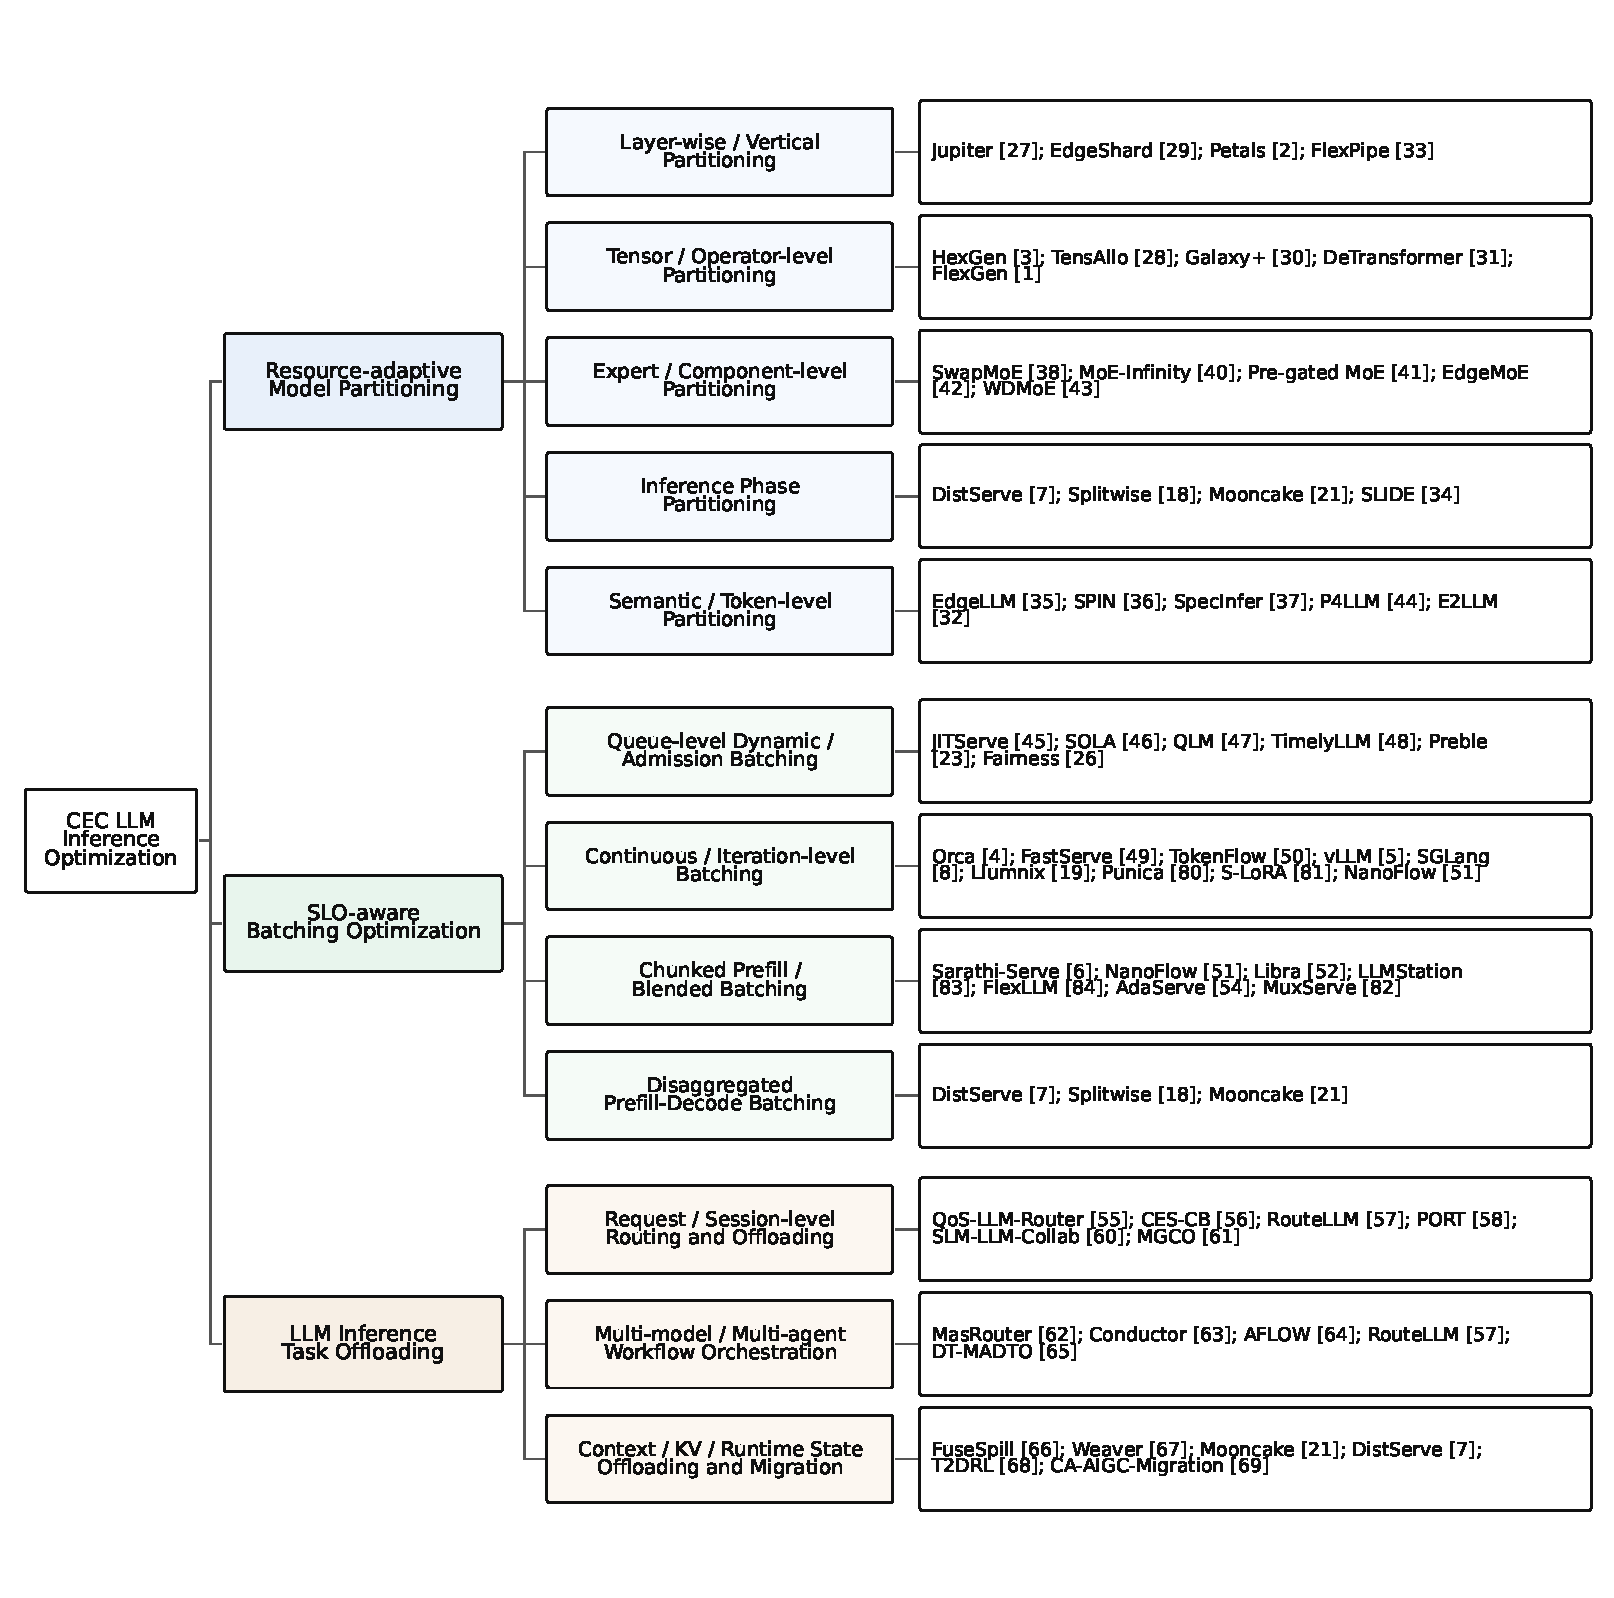
\includegraphics[width=\textwidth]{figures/cec_llm_optimization_overview_taxonomy.pdf}
    \caption{\textbf{CEC LLM inference 优化主线、子分类与代表工作总览}}
    \label{fig:cec-taxonomy}
\end{figure}

\phantomsection
\subsection*{3.5 小结}
\addcontentsline{toc}{subsection}{3.5 小结}

本章从系统形态出发，说明 CEC LLM inference 由多个异构边缘节点协作提供服务。相较数据中心环境，CEC 需要进一步处理资源异构、网络波动、局部请求池规模有限、用户移动、状态连续性和隐私边界等约束，使模型部署、实例内调度和跨节点服务路径使用一致的资源与状态信息。

按照“优化对象--执行范围”分类，CEC 中的 Model-Level 更关注模型表示和结构能否适配目标设备，Kernel-Level 更关注异构硬件的算子支持与执行效率，Runtime-Level 需要同时管理模型切分执行、网络、状态、batch 和执行流水线，Serving Policy \& Routing-Level 则联合选择执行节点与状态处理方式。

基于这些变化，本报告后续围绕三类 CEC LLM inference 优化主线展开：CEC 下的资源自适应模型部署方法、CEC 中的业务感知 batching 参数优化算法，以及 CEC 中的 LLM inference task offloading。

\clearpage
\phantomsection
\section*{四、CEC 下的资源自适应的模型切分部署方法}
\addcontentsline{toc}{section}{四、CEC 下的资源自适应的模型切分部署方法}

大语言模型推理在 CEC 场景下面临的首要问题，不只是单个模型能否放入某个设备，而是同一次推理中的模型结构、计算阶段和运行时状态能否被合理分布到端侧、接入边缘、区域边缘和云端。端侧设备靠近用户并具有隐私优势，但算力、内存、功耗和散热约束严格；边缘节点提供近用户算力，却常常呈现资源碎片化、设备异构和负载波动；云端算力充足，但网络往返、带宽消耗和数据出域风险会进入端到端服务路径。模型切分部署的价值，正是在这些资源边界之间重新组织一次推理，使大模型不再被单个节点的容量和位置限制。Petals 说明大模型可以通过协作式 block 放置突破单节点容量限制 \cite{borzunov2023petals}，HexGen 说明异构 GPU 和异构网络会改变生成式推理的并行策略 \cite{jiang2023hexgen}，FlexGen 则从单 GPU 场景展示权重、activation 和 KV Cache 的分层放置对吞吐的影响 \cite{sheng2023flexgen}。这些工作共同表明，LLM 推理的部署瓶颈通常同时来自模型权重、activation、KV Cache、互联带宽和运行时调度，而不是单一计算瓶颈。
与一般服务路由不同，模型切分部署关心的是推理内部的执行结构是否发生变化。仅在多个完整模型或完整服务实例之间选择执行路径的方法，本质上属于服务路径选择或负载均衡；它可能影响时延和成本，但没有切分模型本体，也没有改变一次推理中计算、状态或生成职责的组织方式。因此，本章只讨论会改变模型执行拓扑、层内并行方式、推理阶段边界或 token 生成职责分工的方法。这样的边界可以避免把“请求发到哪里”和“模型如何被拆开执行”混为一谈，也便于比较不同方法真正改变的系统对象。
本章将 request-level routing 排除在模型切分部署之外，是为了保持分类口径一致；若请求路由同时触发模型段迁移、阶段迁移或 expert 组件迁移，则其模型执行结构变化部分仍可纳入本章讨论。
本文按 primary optimization object 将相关方法划分为五类：
\begin{enumerate}
\item \textbf{Layer-wise / Vertical Partitioning}：切的是 Transformer 深度方向，决定 layer、block 或 model shard 放在哪些节点上执行。
\item \textbf{Tensor / Operator-level Partitioning}：切的是同一层内部的计算单元，决定 attention head、MLP 矩阵、tensor shard 或 communication primitive 如何并行。
\item \textbf{Expert / Component-level Partitioning}：切的是 MoE expert 等模型组件，决定哪些 expert 常驻、换入、映射或跨层级放置。
\item \textbf{Inference Phase Partitioning}：切的是 prefill、decode、verification、download 等执行阶段，利用不同阶段的资源画像差异。
\item \textbf{Semantic / Token-level Partitioning}：切的是生成过程本身，决定 draft、verify、semantic segment、token-wise partition 等语义单元如何协作。
\end{enumerate}

这五类方法不是严格互斥的。Jupiter 同时涉及边缘协作执行和 prefill/decode 阶段组织 \cite{ye2025jupiter}；TensAllo 同时包含设备选择、模型部署和张量并行 \cite{zhang2025tensallo}；Mooncake 以 prefill/decode 解耦为主，但其收益依赖分布式 KV Cache \cite{qin2025mooncake}；SwapMoE 则更接近专家级动态驻留与换入 \cite{kong2024swapmoe}。本文按主要优化对象归类，交叉关系在总览表中保留。这个口径的目的不是把每篇工作强行放进唯一格子，而是让读者能看清：某个方法到底是在切模型深度、切层内计算、切专家组件、切执行阶段，还是切生成语义。

表中“切分类型”表示论文中最接近本章 taxonomy 的主优化对象，不等价于论文全部贡献。例如 Mooncake 的核心贡献包含 KVCache-centric 架构，本章将其放入阶段切分，是因为其服务路径首先建立在 prefill/decode disaggregation 之上 \cite{qin2025mooncake}。

表~\ref{tab:cec-model-partition-overview} 汇总了本章五类模型切分部署方法的代表工作、发表位置、切分类型、优化目标与加速机制；图~\ref{fig:cec-model-partition-taxonomy} 进一步以树状结构展示五类方法、主要切分对象和代表工作之间的对应关系。

\begingroup
\scriptsize
\setlength{\tabcolsep}{1.4pt}
\renewcommand{\arraystretch}{1.35}
\emergencystretch=2em
\begin{longtable}{@{}>{\raggedright\arraybackslash\hspace{0pt}}p{0.035\textwidth} >{\raggedright\arraybackslash\hspace{0pt}}p{0.205\textwidth} >{\raggedright\arraybackslash\hspace{0pt}}p{0.085\textwidth} >{\raggedright\arraybackslash\hspace{0pt}}p{0.105\textwidth} >{\raggedright\arraybackslash\hspace{0pt}}p{0.105\textwidth} >{\raggedright\arraybackslash\hspace{0pt}}p{0.155\textwidth} >{\raggedright\arraybackslash\hspace{0pt}}p{0.270\textwidth}@{}}
\caption{\textbf{CEC 下资源自适应模型切分部署方法相关工作}}
\label{tab:cec-model-partition-overview}\\
\toprule
\textbf{序号} & \textbf{System / Framework} & \textbf{Venue / Year} & \textbf{切分类型} & \textbf{Objectives} & \textbf{Optimization Technology} & \textbf{加速机制 / 方法核心} \\
\midrule
1 & Jupiter: Fast and Resource-Efficient Collaborative Inference of Generative LLMs on Edge Devices \cite{ye2025jupiter} & IEEE INFOCOM 2025 & 层级切分 / 推理阶段切分 & prefill/decode 协同执行 & intra-sequence pipeline parallelism; outline-based pipeline parallel decoding; speculative decoding & Prefill 阶段用序列内流水线并行分摊长 prompt 计算；decode 阶段用 outline-based pipeline parallel decoding 和 speculative decoding 减少自回归串行步数与流水线气泡 \\
\tabrowrule
2 & TensAllo: Adaptive Deployment of LLMs on Resource-Constrained Heterogeneous Edge Devices \cite{zhang2025tensallo} & IEEE INFOCOM 2025 & 层级切分 / 张量切分 & 在资源受限异构边缘设备上部署 LLM & adaptive device selection; tensor allocation; tensor parallelism; quantization & 通过设备选择和 tensor allocation 把计算分配到更合适的异构设备；再用量化降低内存占用，使更多 tensor shard 能留在边缘设备上执行 \\
\tabrowrule
3 & EdgeShard: Efficient LLM Inference via Collaborative Edge Computing \cite{zhang2024edgeshard} & IEEE IoT Journal 2025 & 层级切分 / 垂直切分 & 模型分片放置 & model shard placement; joint device selection; dynamic programming & 将 LLM 切成 model shards，并联合选择设备和 shard placement；动态规划寻找计算时延、传输代价和 pipeline 吞吐之间更优的放置方案 \\
\tabrowrule
4 & Petals: Collaborative Inference and Fine-tuning of Large Models \cite{borzunov2023petals} & ACL 2023 Demo & 层级切分 / 垂直切分 & 将大模型 block 分布到多个参与节点 & decentralized layer/block placement; pipeline across volunteered servers & 把 Transformer block 分散存放在志愿节点 GPU 上，客户端按 pipeline 顺序调用连续 block，避免本地 RAM/SSD offloading 反复搬运完整权重 \\
\tabrowrule
5 & HexGen: Generative Inference of Large Language Model over Heterogeneous Environment \cite{jiang2023hexgen} & ICML 2024 & 层级切分 / 张量切分 & 在异构 GPU 和异构网络上组织生成式推理 & asymmetric tensor parallelism; pipeline parallelism; constrained scheduling & 同时允许 pipeline stage 和 tensor parallel degree 非对称配置，让快慢 GPU、异构链路承担不同计算份额，而不是强制所有 stage 使用同构并行度 \\
\tabrowrule
6 & Resource-Efficient Collaborative Edge Transformer Inference With Hybrid Model Parallelism \cite{ye2025resource} & IEEE TMC 2025 & 层级切分 / 张量切分 & 混合并行协同推理 & hybrid model parallelism; heterogeneity- and memory-aware planning; communication overlap & 用 hybrid model parallelism 结合 layer/pipeline 与 tensor 并行；通过 ReduceScatter/AllGather 替代部分 AllReduce，并用通信-计算重叠降低边缘弱链路上的同步等待 \\
\tabrowrule
7 & Co-Designing Transformer Architectures for Distributed Inference With Low Communication \cite{du2024co} & IEEE TPDS 2025 & 张量/算子级切分 & 降低分布式 Transformer 推理通信 & low-communication architecture co-design; block parallelism; two-phase planning & 通过把原 Transformer layer 重构为多个 decoupled sub-block 暴露 block parallelism，减少层内强依赖和 all-reduce 次数，再用离线权重放置与在线并行规划选择低通信执行路径 \\
\tabrowrule
8 & FlexGen: High-throughput Generative Inference of Large Language Models with a Single GPU \cite{sheng2023flexgen} & ICML 2023 & 张量/算子级切分 & 在单 GPU 资源受限环境中服务大模型 & tensor/KV/activation placement; GPU-CPU-disk offloading; linear programming & 把权重、activation 和 KV cache 在 GPU、CPU、磁盘之间分层放置，用线性规划选择 offloading 和访问模式，并结合压缩扩大 batch size 与吞吐 \\
\tabrowrule
9 & E2LLM: Structure-Guided Efficient Inference for LLMs in Distributed Edge-IoT Environments \cite{feng20262} & IEEE TMC 2026 & 推理阶段切分 / 语义级协同切分 & 边缘结构规划与 IoT 并行解码 & structure-guided planning; static-dynamic KV cache partitioning; distributed decoding & 边缘节点负责结构规划和 segment-specific KV 生成，IoT 设备并行执行轻量 decoding；静态/动态 KV 分离减少重复传输，并用 response skeleton 保持片段语义一致 \\
\tabrowrule
10 & FlexPipe: Adapting Dynamic LLM Serving Through Inflight Pipeline Refactoring in Fragmented Serverless Clusters \cite{lin2026flexpipe} & EuroSys 2026 & 层级切分 / 垂直切分 & 运行时 pipeline stage 重构 & fine-grained model partitioning; inflight pipeline refactoring; topology-aware allocation & 将模型预切成细粒度 stage，并在请求执行中动态调整 pipeline granularity；通过一致的 cache transition 和拓扑感知资源分配适配碎片化 GPU \\
\tabrowrule
11 & DistServe: Disaggregating Prefill and Decoding for Goodput-optimized LLM Serving \cite{zhong2024distserve} & OSDI 2024 & 推理阶段切分 & prefill/decode 物理解耦 & phase-specific workers; phase-aware parallelism; KV transfer & 将 compute-heavy prefill 与 memory/latency-sensitive decode 分配给不同 worker pool；分别选择并行度和 batch 策略，再通过 KV transfer 连接两阶段 \\
\tabrowrule
12 & Splitwise: Efficient Generative LLM Inference Using Phase Splitting \cite{patel2024splitwise} & ISCA 2024 & 推理阶段切分 & prompt/token 阶段分离 & prompt pool; token pool; hardware matching; overlapped KV transfer & 将 prompt computation 和 token generation 拆到不同机器池，使两阶段匹配不同硬件；同时用 layer-wise/overlapped KV transfer 降低阶段切换的关键路径开销 \\
\tabrowrule
13 & Mooncake: Trading more storage for less computation -- A KVCache-centric architecture for serving LLM chatbot \cite{qin2025mooncake} & USENIX FAST 2025 & 推理阶段切分 & prefill/decode disaggregation & distributed KV cache; global scheduling; KVCache-centric architecture & 在 prefill/decode 解耦基础上构建分布式 KVCache，把 CPU、DRAM、SSD、NIC 作为共享状态层；调度器按 KV 复用、本地性和 SLO 选择 prefill/decode 实例 \\
\tabrowrule
14 & SLIDE: Simultaneous Model Downloading and Inference at the Wireless Network Edge \cite{qu2026slide} & IEEE TMC 2026 & 推理阶段切分 & 下载与推理重叠 & layer-wise download/inference overlap; bandwidth and compute allocation & 按 layer 递归依赖组织下载和执行：用户一边接收后续 layer，一边执行已下载 layer；联合优化带宽和计算分配以隐藏模型下载等待 \\
\tabrowrule
15 & EdgeLLM: Fast On-Device LLM Inference With Speculative Decoding \cite{xu2024edgellm} & IEEE TMC 2025 & 语义/token 级协同切分 & 减少端侧逐 token 解码开销 & on-device speculative decoding; branch navigation; self-adaptive fallback; compute-I/O pipeline & 小 draft LLM 常驻内存生成候选 token，大 target LLM 批量验证；用分支导航避免把算力浪费在低概率分支，并用 compute-I/O pipeline 隐藏大模型权重加载 \\
\tabrowrule
16 & SPIN: Accelerating Large Language Model Inference with Heterogeneous Speculative Models \cite{chen2025spin} & IEEE INFOCOM 2025 & 语义/token 级协同切分 & 异构草稿模型选择与验证流水线 & heterogeneous SSM selection; request decomposition; speculation/verification pipelining & 为不同难度请求选择合适的异构 speculative model；把长请求拆分以降低 verification batch padding，并流水化 speculation 与 verification 阶段 \\
\tabrowrule
17 & SpecInfer: Accelerating Large Language Model Serving with Tree-based Speculative Inference and Verification \cite{miao2024specinfer} & ASPLOS 2024 & 语义/token 级协同切分 & token tree 草稿与批量验证 & tree-based speculative inference; parallel verification & 多个小模型生成候选 token tree，目标 LLM 不再逐 token 增量生成，而是作为 verifier 一次并行校验多条候选路径，从而减少目标模型调用次数 \\
\tabrowrule
18 & SwapMoE: Serving Off-the-shelf MoE-based Large Language Models with Tunable Memory Budget \cite{kong2024swapmoe} & ACL 2024 & 专家/组件级切分 & 专家驻留可调 & virtual experts; expert swapping; tunable memory budget & 只把动态选择的重要专家作为 virtual experts 常驻主存，其余专家按需映射和换入，在不剪枝模型结构的情况下减少 MoE 推理内存占用和换入开销 \\
\tabrowrule
19 & Taming Latency-Memory Trade-Off in MoE-Based LLM Serving via Fine-Grained Expert Offloading \cite{yu2026taming} & EuroSys 2026 & 专家/组件级切分 & 细粒度 expert offloading & fine-grained expert offloading; latency-memory trade-off & 以 expert 为换入/卸载单元，在显存预算下决定哪些专家保留在 GPU、哪些下沉到主机或存储层，从而在显存节省和专家加载延迟之间折中 \\
\tabrowrule
20 & MoE-Infinity: Efficient MoE Inference on Personal Machines with Sparsity-Aware Expert Cache \cite{xue2024moe} & ICML 2025 & 专家/组件级切分 & 稀疏感知 expert cache & sparsity-aware expert cache; expert prefetching; memory hierarchy & 利用 MoE token 路由稀疏性和专家访问局部性，只缓存即将使用或高频专家，并通过预取和分层内存降低专家缺页造成的 decode 停顿 \\
\tabrowrule
21 & Pre-gated MoE: An Algorithm-System Co-Design for Fast and Scalable MoE Inference \cite{hwang2024pre} & ISCA 2024 & 专家/组件级切分 & 提前 expert routing 与系统协同 & pre-gating; expert scheduling; algorithm-system co-design & 在系统执行前更早获得 expert 选择信息，使 expert 加载、通信和调度可以提前安排，减少 MoE 推理中的路由等待和跨设备同步 \\
\tabrowrule
22 & EdgeMoE: Empowering Sparse Large Language Models on Mobile Devices \cite{yi2025edgemoe} & IEEE TMC 2025 & 专家/组件级切分 & 移动端稀疏 LLM 部署 & sparse MoE deployment; expert management; on-device inference & 面向移动设备资源约束管理 MoE expert 的驻留与执行，使稀疏大模型能够在端侧或近端资源上以可控内存开销运行 \\
\tabrowrule
23 & WDMoE: Wireless Distributed Mixture of Experts for Large Language Models \cite{xue2025wdmoe} & IEEE TWC 2025 & 专家/组件级切分 & 无线边缘分布式 MoE & wireless distributed experts; expert selection; bandwidth allocation & 将 gating/attention 和 experts 分布在基站与移动设备之间，根据 expert 权重、设备延迟和无线带宽联合选择专家与分配通信资源 \\
\tabrowrule
24 & P4LLM: Protecting Embedding Privacy against Model Inversion Attacks for EaaS LLM Serving via Token-wise Partition and Perturbation \cite{lu2026p4llm} & IEEE TMC 2026 & 语义/token 级协同切分 & token-wise partition + perturbation & insensitive token filtering; partitioning scheduler; hidden-state perturbation & 在用户侧按 token 切分 Transformer 执行，只对敏感 token 的 hidden state 做扰动并上传，非敏感 token 过滤或轻处理，从而减少扰动计算和传输负担 \\
\bottomrule
\end{longtable}
\endgroup

\begin{figure}[!htbp]
\centering
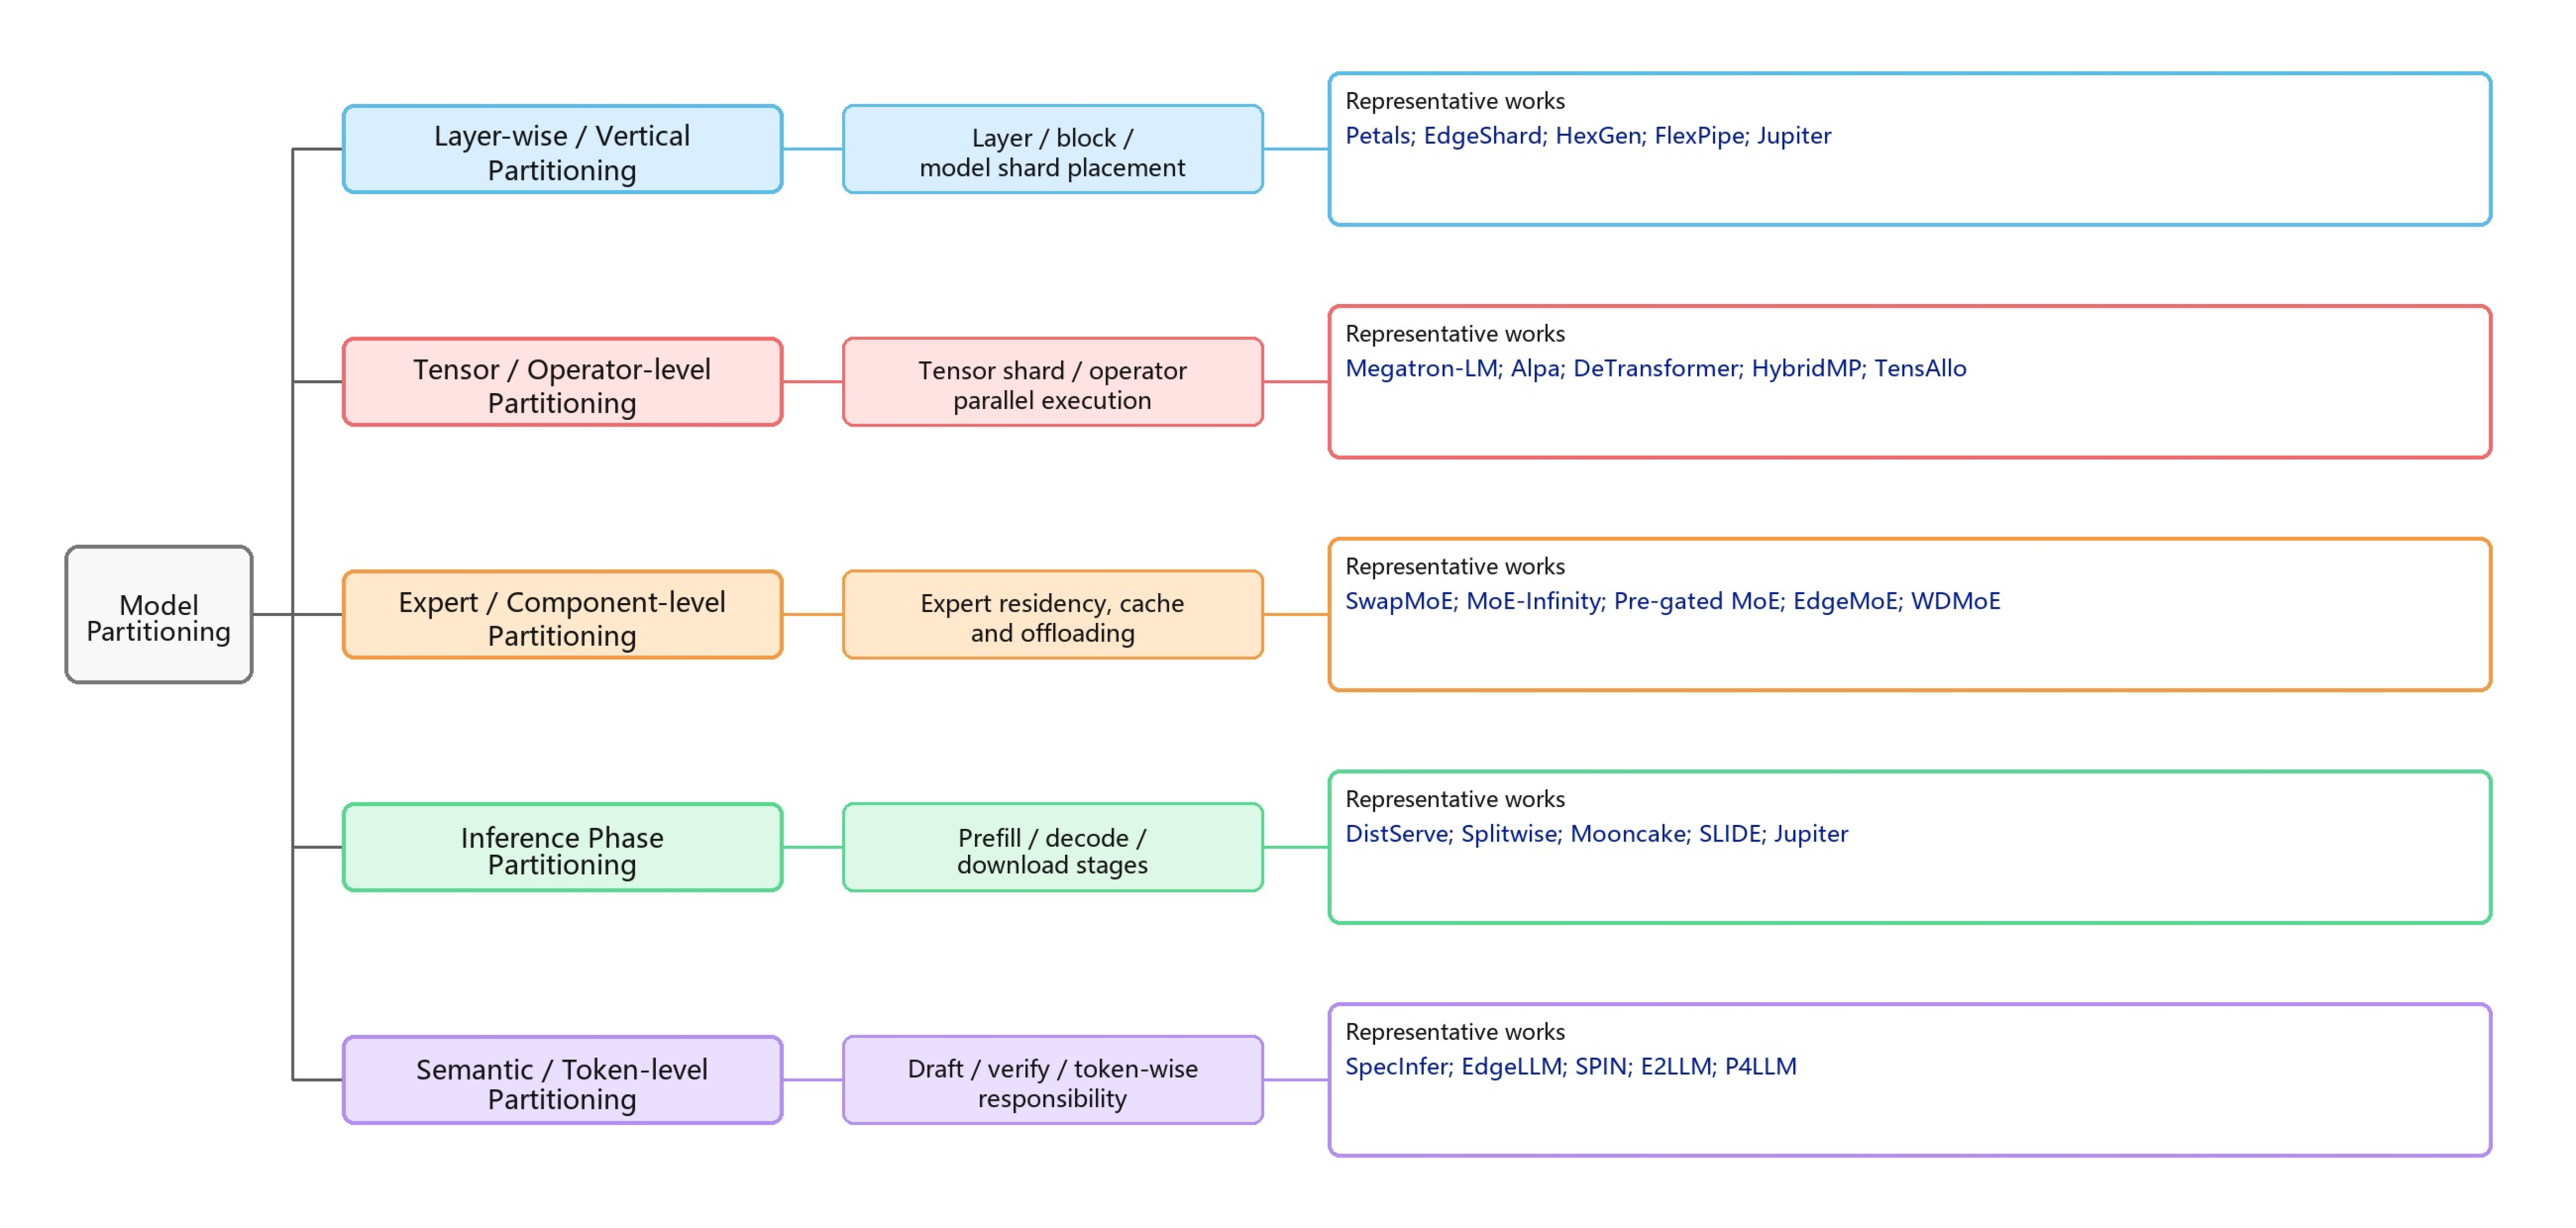
\includegraphics[width=\textwidth]{figures/ch4_model_partition_taxonomy.pdf}
\caption{\textbf{CEC 下资源自适应模型切分部署方法的分类树}}
\label{fig:cec-model-partition-taxonomy}
\end{figure}


\phantomsection
\subsection*{4.1 Layer-wise / Vertical Partitioning}
\addcontentsline{toc}{subsection}{4.1 Layer-wise / Vertical Partitioning}
层级切分是最接近传统意义上“模型分割”的一类方法。它把 Transformer 视为由多个顺序 block 组成的计算链，在 layer 或 block 边界上拆分模型，并将不同模型段放置到端侧、边缘或云端节点执行。对于无法完整加载模型权重、activation 和运行时状态的端侧或边缘设备，层级切分提供了一种直接的扩展方式：单个节点不再承担完整模型，而是多个节点共同完成同一次 forward。Petals 展示去中心化 block 放置 \cite{borzunov2023petals}，EdgeShard 面向边缘 shard placement \cite{zhang2024edgeshard}，HexGen 讨论异构生成式推理 \cite{jiang2023hexgen}，FlexPipe 则关注 serverless 集群中的 pipeline 重构 \cite{lin2026flexpipe}；这些工作共同验证了沿深度方向拆分模型的价值。

为了把这种“沿深度方向展开”的执行方式与普通请求路由区分开，可以参考图~\ref{fig:ch4-layerwise-partitioning}。
\begin{figure}[!htbp]
\centering
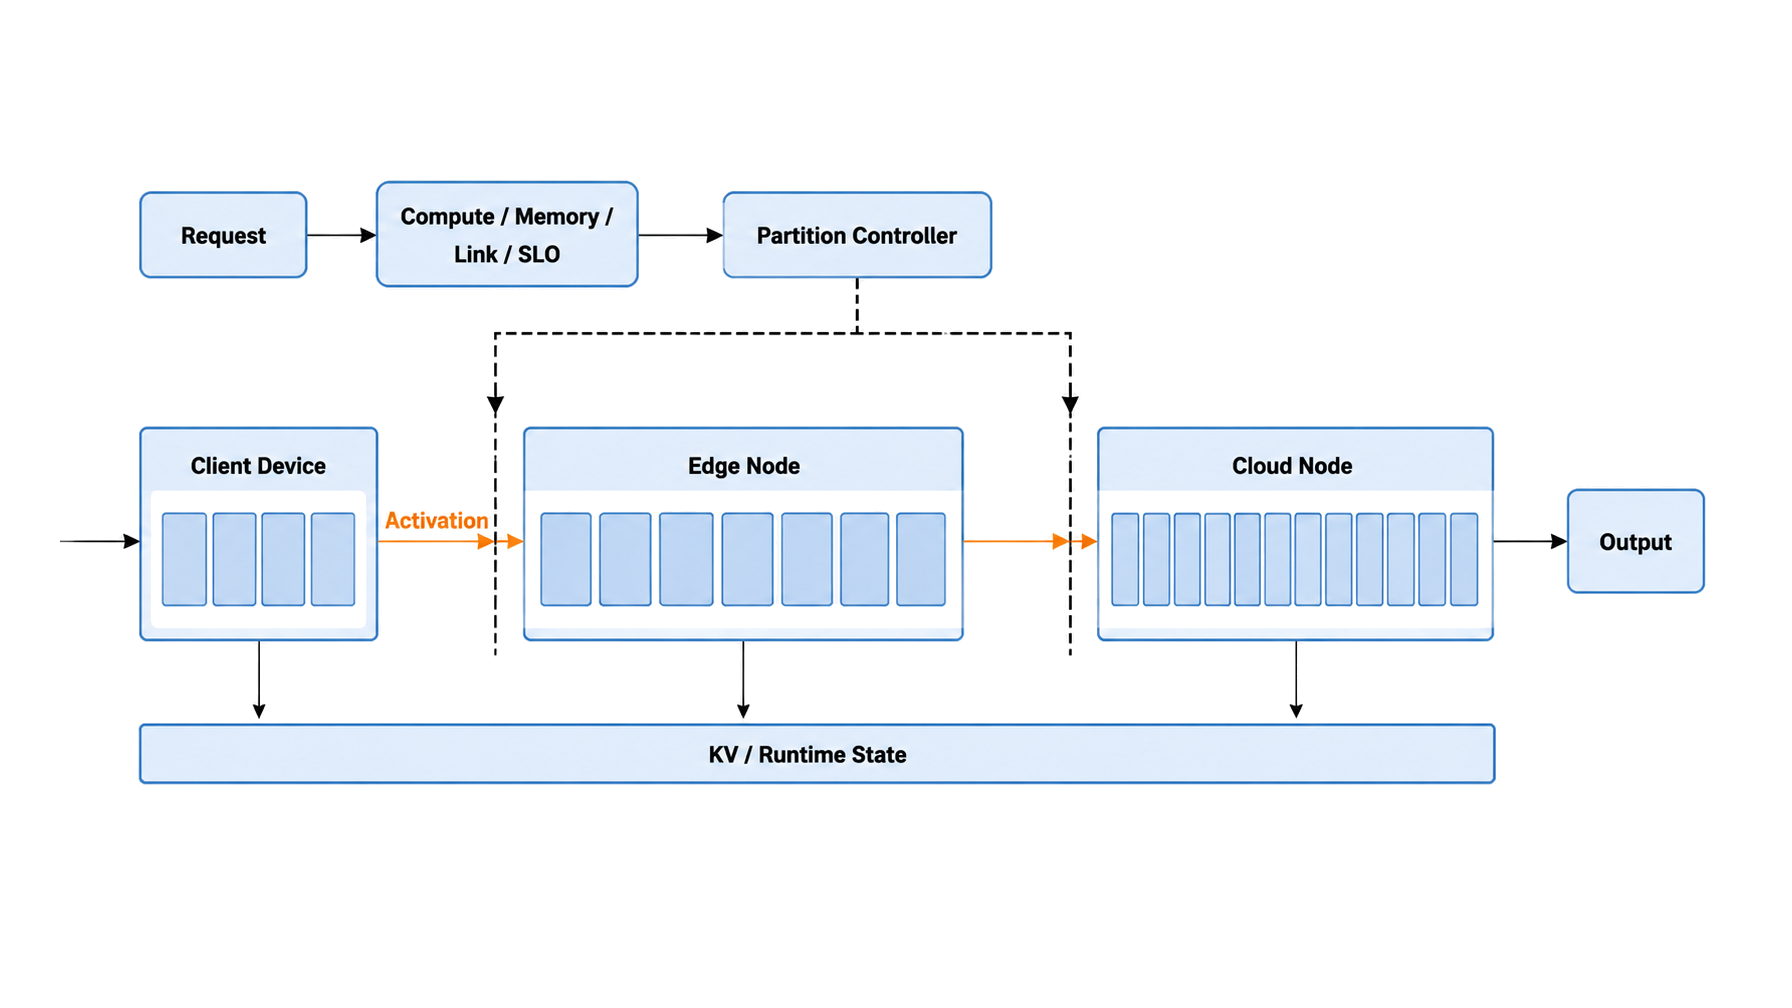
\includegraphics[width=\textwidth]{figures/ch4_2_layerwise_vertical_partitioning.png}
\caption{\textbf{Layer-wise / Vertical Partitioning 机制示意图}}
\label{fig:ch4-layerwise-partitioning}
\end{figure}
示意图中横向排列的 Transformer layers 表示同一个模型在深度方向上的执行链，虚线边界表示可选 split point。Client、Edge 和 Cloud 并不对应固定层数，而是代表不同资源层级；层间箭头表示 activation 或 hidden state 的跨节点传输，KV/state sidecar 表示推理过程中需要伴随模型段管理的运行时状态。Partition Controller 根据链路状态、显存余量、节点负载和 SLO 选择 layer placement、pipeline stage 与 fallback path。因此，层级切分的关键不是平均切开模型，而是在计算节省和跨节点状态传输之间动态权衡。

这一类方法的核心不是“把模型平均切开”，而是寻找合适的 split point 和 placement。切分点靠前，可以减轻端侧计算和内存压力，但会更早产生跨节点 hidden state 或 activation 传输；切分点靠后，可以降低网络依赖，却要求端侧执行更多 layer。对于长上下文请求，activation 规模和 KV 状态增长会进一步放大通信成本；对于短请求，通信启动时延可能抵消计算节省。因此，层级切分通常需要同时估计每层计算量、activation 大小、显存占用、链路带宽、RTT、节点负载和功耗约束。

CEC 环境使层级切分比云端 pipeline parallelism 更难。数据中心内的互联带宽相对稳定，而端-边、边-边、边-云链路可能受到无线抖动、跨域转发和拥塞影响。一个在静态 profiling 中最优的切点，到了移动用户、突发请求或边缘节点过载时可能迅速失效。因此，资源自适应的层级切分往往需要三类能力：离线阶段建立 layer-level profile，在线阶段根据节点和链路状态选择切点，运行时阶段在负载变化时进行有限频率的重配置。GPipe 体现了 pipeline parallelism 在稳定集群中的基本价值 \cite{huang2019gpipe}，Megatron-LM 展示了大模型 tensor parallelism 的基础路线 \cite{narayanan2021efficient}，Alpa 则进一步自动化 inter-operator 与 intra-operator parallelism \cite{zheng2022alpa}。CEC 需要在这些并行思想之上继续纳入异构链路和在线状态。

这类方法还要处理流水线稳定性。切分后，每个模型段的执行时间如果差异过大，较慢节点会成为 pipeline bottleneck；中间节点失败或链路恶化时，后续 layer 是否迁移、是否重新选择切点、是否回退到云端完整执行，都会影响服务连续性。对于 CEC LLM 推理，层级切分不能只作为部署算法讨论，还必须和 admission control、状态管理和异常回退衔接。

总体来看，层级切分适合模型容量和单节点部署能力不足的场景，尤其适用于模型段执行时间差异明显、节点间链路相对稳定、跨节点 activation 可控的系统。它的主要风险在于切分收益被网络传输和流水线等待抵消。因此，CEC 中的层级切分更适合采用“少量稳定切点 + 在线代价修正”的方式，而不是频繁改变模型执行拓扑。

这里的“少量稳定切点”并不意味着静态平均切分，而是指将在线搜索限制在经过 profiling 验证、可部署且不会 OOM 的候选切点集合内，避免运行时任意切分造成模型重加载和状态迁移震荡。
\phantomsection
\subsection*{4.2 Tensor / Operator-level Partitioning}
\addcontentsline{toc}{subsection}{4.2 Tensor / Operator-level Partitioning}
当层级切分仍不足以缓解单层计算和显存压力时，系统需要进入更细粒度的张量/算子级切分。LLM 的每一层内部包含 attention、QKV projection、MLP、归一化和通信同步等多个计算单元，其中 attention head、矩阵乘和中间 activation 都可能成为单设备瓶颈。张量/算子级切分不再以完整 block 为边界，而是在同一层内部拆分 tensor、head、矩阵维度或 operator 执行路径。Megatron-LM 和 Alpa 代表了数据中心大模型中 tensor / intra-operator parallelism 的基础路线 \cite{narayanan2021efficient}, \cite{zheng2022alpa}；DeTransformer 通过结构协同设计降低分布式推理通信 \cite{du2024co}，Galaxy+ 采用混合模型并行组织边缘 Transformer 推理 \cite{ye2025resource}，TensAllo 则把异构边缘设备选择和 tensor allocation 纳入部署决策 \cite{zhang2025tensallo}。

层内拆分的系统关系可以用图~\ref{fig:ch4-tensor-operator-partitioning} 概括，它突出的是同一 Transformer 层内部的并行和同步，而不是层与层之间的顺序切点。
\begin{figure}[!htbp]
\centering
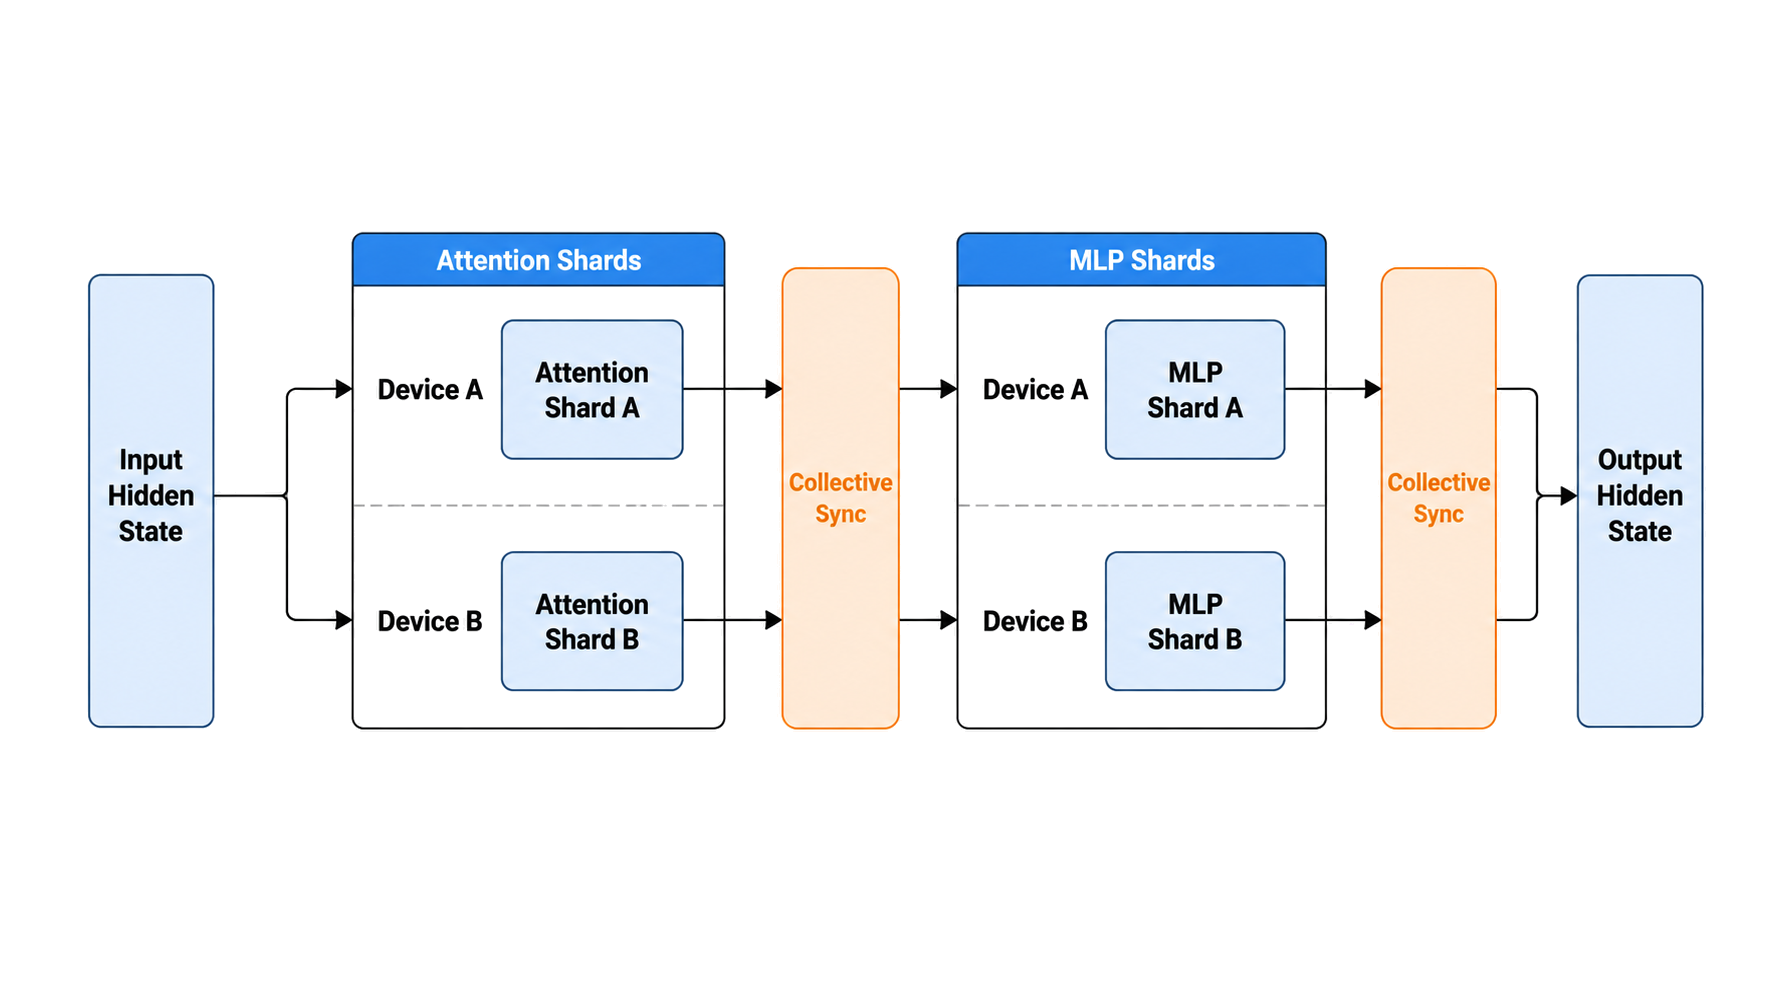
\includegraphics[width=\textwidth]{figures/ch4_3_tensor_operator_partitioning.png}
\caption{\textbf{Tensor / Operator-level Partitioning 机制示意图}}
\label{fig:ch4-tensor-operator-partitioning}
\end{figure}
图中没有展开每个 GEMM 或 attention kernel 的细节，而是保留张量/算子级切分最关键的执行关系：左侧是单个 Transformer layer，中间的 Partition Planner 根据 layer profile、硬件拓扑、显存预算和 SLO 判断是否需要层内并行；右侧的 Device Group 表示同一层被分配到多个 Ascend 设备上执行。Attention 部分可以按 head 或 QKV shard 拆分，MLP 部分可以按矩阵维度拆分；各设备得到局部结果后，再通过 all-gather、reduce-scatter 或 all-reduce 完成同步合并。这里的关键不是“多设备一定更快”，而是并行度增加后同步次数和链路依赖也会增加；在 CEC 中，边缘链路的带宽和抖动会直接决定水平切分是否有收益。

这类方法通常保持模型数学语义不变，改变的是层内计算如何分布到多个设备。它可以表现为 tensor parallelism、hybrid model parallelism、block parallelism、低通信 Transformer 结构或 structure-guided partitioning。与层级切分相比，它能更细地利用碎片化资源；与单机 kernel 优化相比，它必须显式处理跨设备通信、同步和拓扑选择。

本章将 Tensor / Operator-level Partitioning 视为比普通 kernel 优化更高一层的系统问题。若某项工作只优化单设备 GEMM/attention kernel，而不改变层内计算的跨设备分布，则不归入本类。

水平切分的核心矛盾是并行收益与通信惩罚。切得越细，单个设备承载的权重、activation 和中间矩阵越少，也更容易把多个弱设备组织起来；但 all-reduce、all-gather、reduce-scatter 或点对点传输会更频繁。切得越粗，通信开销下降，却可能重新遇到显存或算力瓶颈。数据中心可以依赖高速互联吸收一部分同步成本，CEC 中的边缘设备却往往只有普通以太网、无线链路或多跳边缘互联，过细的 tensor parallelism 很容易变成通信密集型执行。

因此，CEC 下的张量/算子级切分需要比云端并行更强的资源画像。调度器要知道哪些设备适合低比特 GEMM，哪些设备适合 attention，哪些设备只能承担较小 tensor shard；还要估计层内同步频率、通信 primitive 的代价和 batch size 对算子效率的影响。某些工作还通过模型结构 co-design 减少层内依赖，使模型天然更适合低通信分布式推理。这说明水平切分不是单纯调大 parallel degree，而是模型结构、设备选择和通信路径的联合设计。

张量/算子级切分适合单层计算或显存压力成为瓶颈的场景，但在 CEC 中不能简单照搬数据中心 tensor parallelism。边缘链路的带宽、抖动和同步延迟会直接决定并行收益是否存在。因此，这类方法应优先与低通信结构、异构设备选择和静态/动态 profiling 结合，并尽量避免让每个 token 都经过高频跨节点同步 \cite{zhang2025tensallo}, \cite{ye2025resource}, \cite{du2024co}。
\phantomsection
\subsection*{4.3 Expert / Component-level Partitioning}
\addcontentsline{toc}{subsection}{4.3 Expert / Component-level Partitioning}
专家/组件级切分主要面向 MoE 等具有显式内部组件选择机制的模型。与普通 dense Transformer 不同，MoE 模型通常在 FFN 部分包含大量 expert，而每个 token 只激活其中少数 expert。这个结构使模型天然具备“组件级可调度性”：系统不一定让所有 expert 同时常驻同一设备，而可以根据 expert 热度、token routing 分布、显存预算、链路状态和请求类型，决定哪些 expert 常驻、哪些按需换入、哪些放在边缘或云端节点上。SwapMoE 从 expert swapping 角度降低显存压力 \cite{kong2024swapmoe}，MoE-Infinity 利用 sparsity-aware expert cache 支撑个人设备上的 MoE 推理 \cite{xue2024moe}，Pre-gated MoE 通过提前 expert routing 协同系统调度 \cite{hwang2024pre}，EdgeMoE 面向移动端稀疏模型部署 \cite{yi2025edgemoe}，WDMoE 则讨论无线分布式 expert 放置和带宽分配 \cite{xue2025wdmoe}。这些工作共同说明，组件级切分已经成为 MoE 推理系统的重要组织方式。

MoE 场景下，组件驻留和 token routing 的关系更适合从图~\ref{fig:ch4-expert-component-partitioning} 这样的分层缓存视角理解。
\begin{figure}[!htbp]
\centering
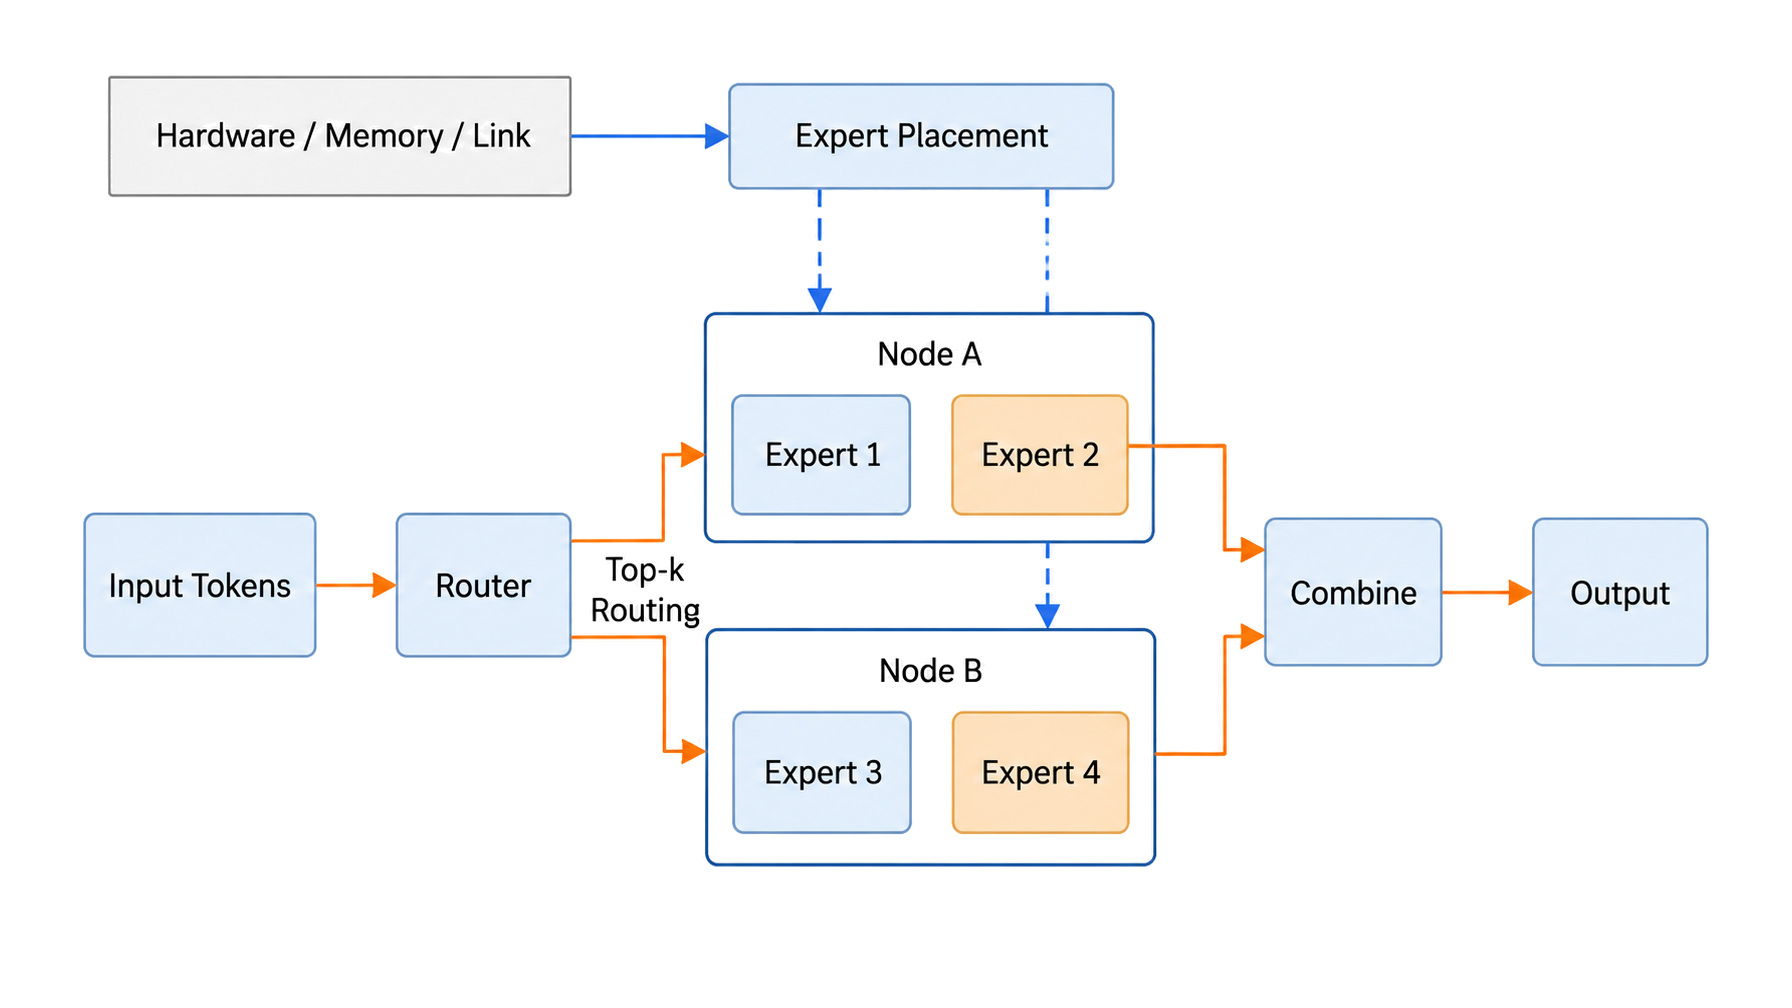
\includegraphics[width=0.86\textwidth]{figures/ch4_4_expert_component_partitioning.png}
\caption{\textbf{Expert / Component-level Partitioning 机制示意图}}
\label{fig:ch4-expert-component-partitioning}
\end{figure}
在这个机制中，MoE Router 为每个 token 选择 top-k experts，Expert Placement Policy 再根据 expert hotness、memory budget 和 link state 决定 expert 的驻留层级。热 expert 可以放入 Edge Expert Cache，次热 expert 放在 Regional Expert Pool，低频或完整 expert 集合保存在 Cloud / SSD Expert Store。箭头表示 token-expert 访问路径和 expert swap/prefetch 路径。组件级切分的收益来自稀疏激活和访问局部性，风险则来自 expert 预测错误后产生的远程访问或换入等待。

这一类方法之所以不直接并入张量/算子级切分，是因为它切的不是矩阵维度或 communication primitive，而是具有模型语义的组件单元。一个 expert 往往对应一组完整参数和计算路径，其是否被激活取决于 token-level routing；系统优化的对象也从“如何并行执行同一层矩阵”转向“如何管理大量稀疏激活组件的驻留、映射和调度”。因此，专家/组件级切分介于层内切分和语义/token 协同之间：它发生在模型内部组件层面，但收益取决于 token 分布和专家访问模式。

在 CEC 场景下，专家/组件级切分的价值在于降低大模型组件的常驻压力。端侧或接入边缘难以保存完整 MoE 模型，但可能保存高频 expert、局部业务相关 expert 或经过压缩的 expert cache；区域边缘可以维护更大的 expert pool；云端则保留完整 expert 集合并处理低频或复杂请求。系统需要在 expert 命中率、换入换出成本、跨节点 expert 访问时延和输出质量之间做权衡。如果 expert 热度预测准确，组件级切分可以减少显存占用并提高边缘可部署性；如果预测失误，频繁 swap 或远程访问 expert 会直接破坏 decode 时延。

专家/组件级切分的决策变量包括 expert residency、expert cache size、expert hotness prediction、token routing statistics、swap bandwidth、memory budget、fallback policy 和跨层级 expert placement。与层级切分相比，它更细粒度；与张量切分相比，它更依赖模型稀疏激活；与语义/token 级协同相比，它仍然保持同一个 MoE 模型内部的 expert 语义一致性，而不是把 draft、verify 或语义段分给不同模型完成。

总体来看，专家/组件级切分适合 MoE 模型、expert 热度具有局部性、边缘节点无法常驻完整 expert 集合的场景。它不应被简单理解为普通 request routing，因为请求仍在同一个 MoE 模型语义下执行；也不应被完全归入 token-level collaboration，因为系统主要调度的是 expert 组件而非生成职责。现有代表工作已经覆盖 expert swapping、fine-grained expert offloading、expert cache、pre-gating 和 wireless distributed experts 等不同角度；CEC 场景下仍然缺少把用户移动、区域业务热度、expert cache 迁移和无线带宽联合起来建模的工作 \cite{yu2026taming}, \cite{xue2025wdmoe}。

若目标模型是 dense LLM，本类方法一般不应作为模型切分部署的主路径；若目标模型或后续业务引入 MoE、专家模型或多 adapter 组件，本类才会成为核心部署问题。
\phantomsection
\subsection*{4.4 Inference Phase Partitioning}
\addcontentsline{toc}{subsection}{4.4 Inference Phase Partitioning}
LLM 推理不是单一形态的计算。Prefill 需要一次性处理完整 prompt，矩阵规模大、并行度高，通常更偏 compute-bound；decode 逐 token 生成，频繁访问 KV Cache，通常更偏 memory-bound 或 latency-bound；speculative decoding 中的 verification 又会形成目标模型批量校验；在无线边缘场景中，模型下载、加载和推理还可能同时出现在关键路径上。推理阶段切分正是利用这些阶段资源画像的差异，把不同阶段放到更合适的节点或资源池上执行。DistServe \cite{zhong2024distserve}、Splitwise \cite{patel2024splitwise} 和 Mooncake \cite{qin2025mooncake} 是 prefill/decode disaggregation 的代表；Jupiter 从边缘协作角度组织 prefill/decode 执行 \cite{ye2025jupiter}，E2LLM 从 Edge-IoT 结构化生成角度扩展阶段分工 \cite{feng20262}，SLIDE 则讨论无线边缘中的下载-推理重叠 \cite{qu2026slide}。

阶段级切分更适合放在推理流水线视角下理解，图~\ref{fig:ch4-inference-phase-partitioning} 给出了 prefill、decode、verification 与 KV/state handoff 的典型组织方式。
\begin{figure}[!htbp]
\centering
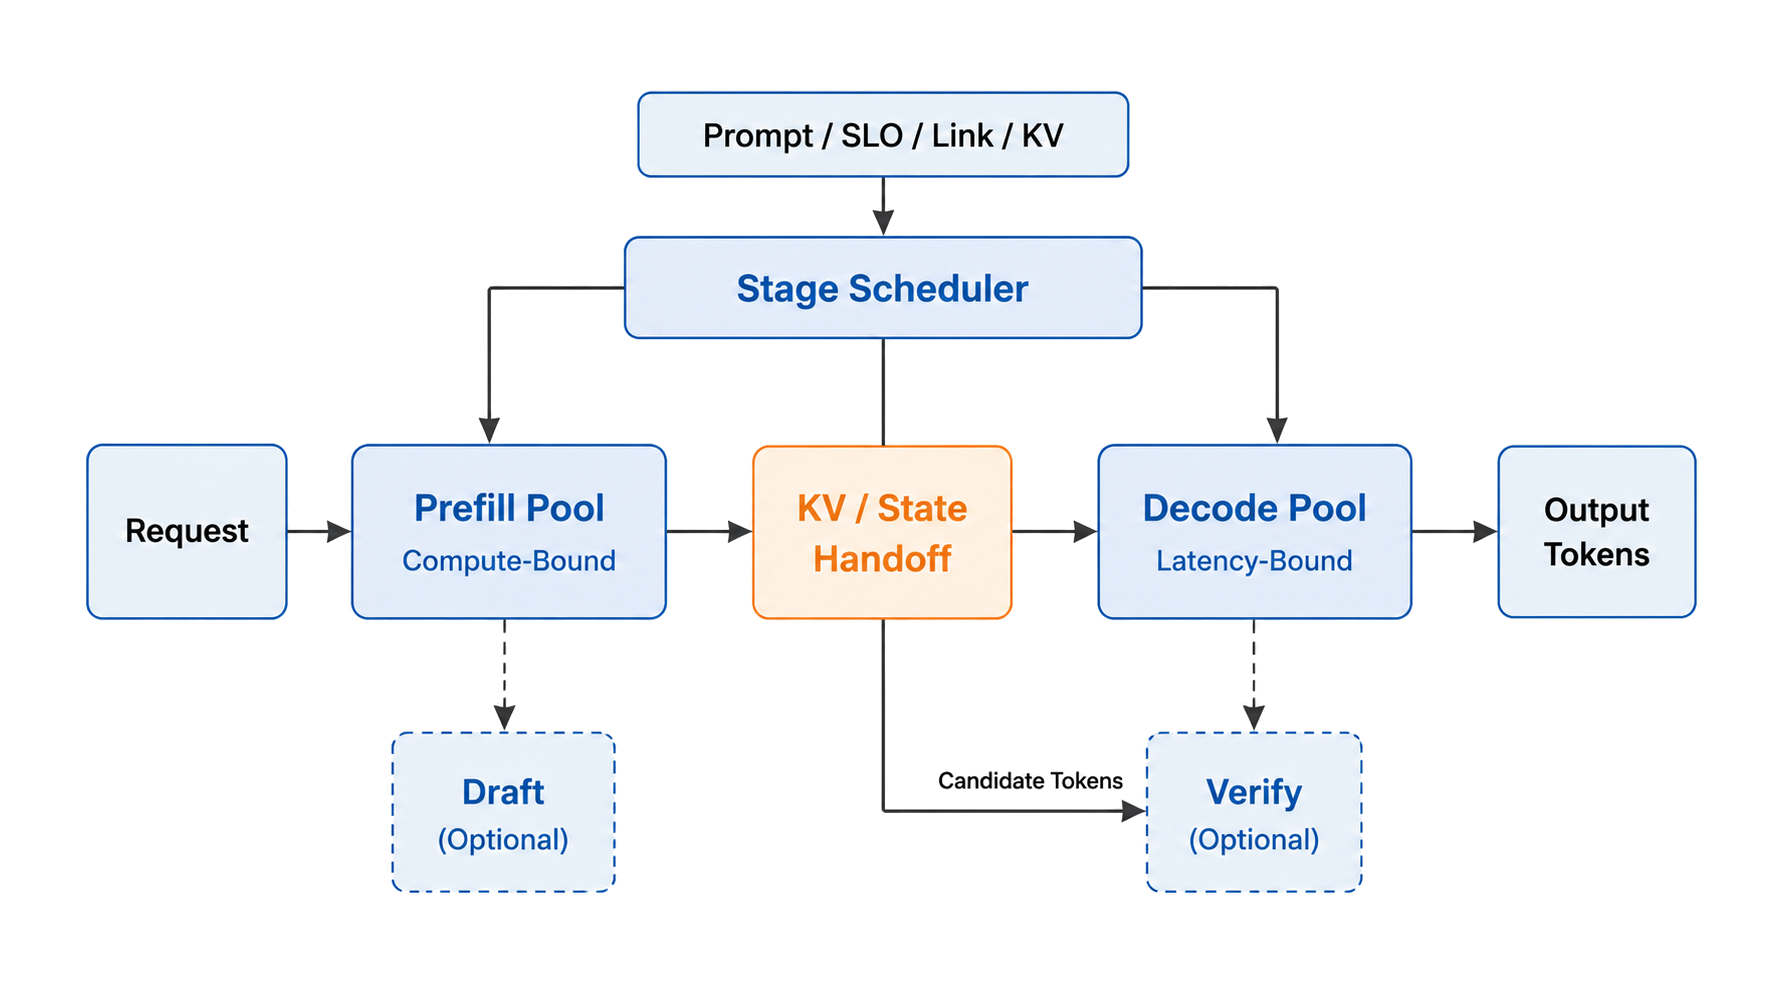
\includegraphics[width=\textwidth]{figures/ch4_5_inference_phase_partitioning.png}
\caption{\textbf{Inference Phase Partitioning 机制示意图}}
\label{fig:ch4-inference-phase-partitioning}
\end{figure}
这里的 Stage Scheduler 根据 prompt length、SLO、link state 和 KV locality 把请求送入不同阶段资源池。Prefill Pool 处理 compute-bound 的 prompt batch，Decode Pool 维护 memory/latency-bound 的 active sequence，KV / State Handoff 负责在阶段之间传递 KV blocks、metadata 和必要状态。若系统引入 verification 或 draft stage，它们也可以作为独立阶段被调度。阶段切分的核心收益来自资源画像匹配和阶段干扰隔离，核心代价则集中在 KV/state 传输与阶段队列协调。

最典型的形式是 prefill/decode disaggregation。长 prompt 的 prefill 可以放在算力更强、吞吐更高的区域边缘或云端实例，低时延 decode 则由更靠近用户的接入边缘承担。这样做可以减少长 prefill 对 decode 的阻塞，也能让不同硬件分别服务 compute-heavy 和 memory-heavy 阶段。进一步地，系统还可以把 draft generation 和 target verification 分开，或将模型下载与推理执行重叠，从而缩短冷启动和模型切换时延。

阶段切分的决策变量包括 prefill worker、decode worker、stage queue、pipeline boundary、KV transfer、verification placement、download/inference overlap 和阶段间同步机制。它的收益来自资源匹配和干扰隔离，但代价集中在状态交接。Prefill 和 decode 共享 KV Cache，draft 和 verify 共享候选 token 与概率校验状态，下载与推理重叠则会竞争网络、存储和内存带宽。换言之，阶段切分能否有效，取决于拆开之后能否低成本地把状态交给下一阶段 \cite{zhong2024distserve}, \cite{patel2024splitwise}, \cite{qin2025mooncake}。

在 CEC 中，阶段切分具有明显的场景价值。接入边缘适合承担低时延 decode，区域边缘适合聚合多个入口的 prefill-heavy 请求，云端适合长上下文、大模型 verification 或复杂推理。但这种分工不是无条件成立：如果 prefill 在云端完成后需要把大量 KV 传回边缘，链路抖动就会直接放大 TTFT 或后续 TPOT；如果边缘并发不足，独立 decode worker 可能无法形成有效 batch；如果用户移动导致入口切换，阶段边界还可能触发状态迁移。因此，阶段切分实际是在阶段资源匹配和状态连续性之间做权衡。

推理阶段切分适合 prefill/decode 负载差异明显、阶段队列规模足够、状态传输可控的场景。若请求很短、边缘并发很低或链路抖动大，复杂阶段拆分可能不如本地顺序执行稳定。因此，阶段切分必须和 KV 状态管理、链路预测、admission control 和回退策略一起设计；它不是独立的部署技巧，而是贯穿推理流水线的资源组织方式。

阶段切分与第五章的 Disaggregated Prefill-Decode Batching 视角不同。第四章关注 prefill/decode 是否跨实例或跨层级部署；第五章关注在已经分离的 prefill pool 与 decode pool 内部如何分别组批、排队和控制参数。
\phantomsection
\subsection*{4.5 Semantic / Token-level Partitioning}
\addcontentsline{toc}{subsection}{4.5 Semantic / Token-level Partitioning}
语义/token 级协同切分与前四类不同。它不一定把同一个模型的 layer、tensor 或 expert 组件拆开，而是把一次生成过程中的职责拆开：草稿由小模型产生，验证由大模型完成；长回答可以按语义段并行生成；隐私敏感 token 或 embedding 可以被单独 partition 和 perturbation。这里“切分”的对象是生成语义和 token 处理职责，而不是模型内部参数组件。SpecInfer 展示 token tree verification \cite{miao2024specinfer}，EdgeLLM 讨论端侧 speculative decoding \cite{xu2024edgellm}，SPIN 关注异构草稿模型选择 \cite{chen2025spin}，E2LLM 则展示语义段级并行生成 \cite{feng20262}。

生成职责级方法的结构可参考图~\ref{fig:ch4-semantic-token-partitioning}。它强调的不是参数如何分片，而是 draft、verify、refine 和 privacy filtering 等职责如何分配。
\begin{figure}[!htbp]
\centering
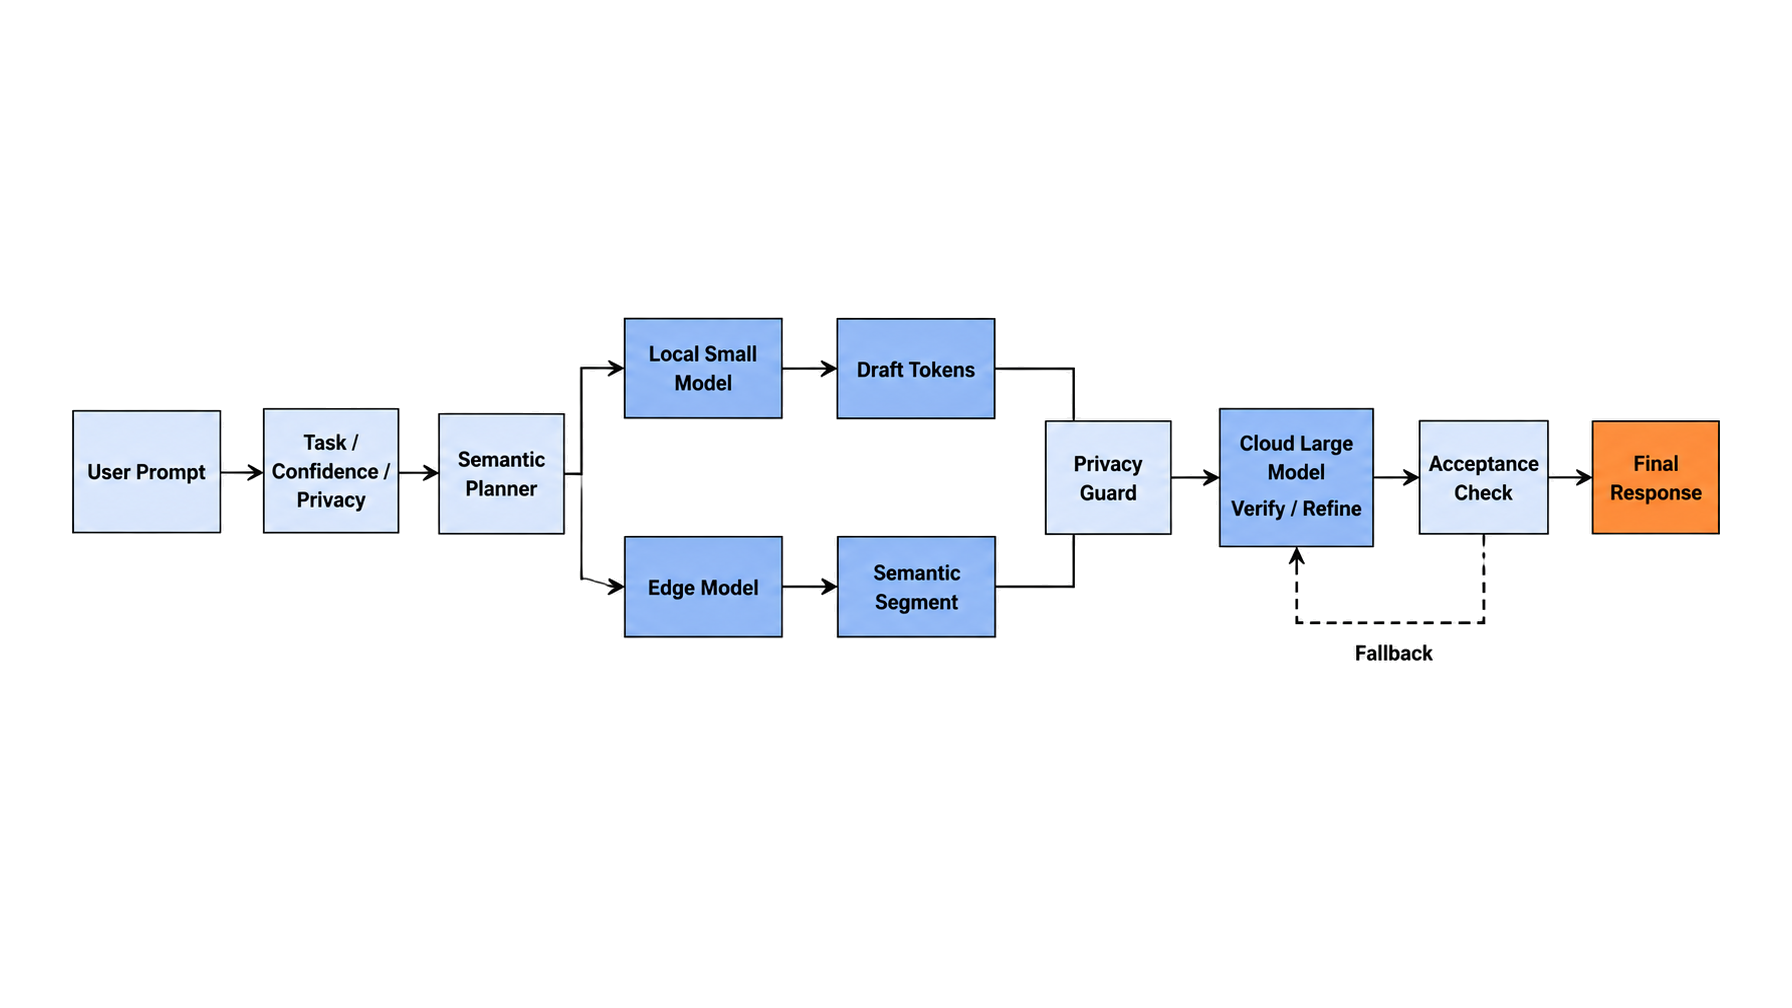
\includegraphics[width=\textwidth]{figures/ch4_6_semantic_token_partitioning.png}
\caption{\textbf{Semantic / Token-level Partitioning 机制示意图}}
\label{fig:ch4-semantic-token-partitioning}
\end{figure}
从系统路径看，Semantic Planner 根据 task type、confidence 和 privacy tag 判断每段生成职责交给哪个模块。Local Small Model 负责生成 draft tokens，Edge Model 可以承担部分 semantic segment generation，Privacy Guard 对敏感 token 做 partition 或 perturbation，Cloud Large Model 负责 verify/refine。Acceptance Check 决定草稿是否接受、是否回退到大模型重算。token/语义级方法的关键约束是质量一致性和错误回退，而不仅是加速。

这类方法的出发点，是自回归生成并不必然只能由一个模型连续完成。系统可以在端侧先生成 draft，再由边缘或云端目标模型 verify；可以先生成 response skeleton，再把不同语义段交给多个设备并行生成；也可以将隐私敏感 token 从普通 token 流中分离出来，采用额外扰动或分区策略。与层级切分和张量切分相比，它改变的是生成过程中的职责边界，而不是纯粹的模型拓扑 \cite{xu2024edgellm}, \cite{lu2026p4llm}。

语义/token 级协同的核心变量包括 draft length、acceptance rate、verification frequency、semantic segment boundary、token partition、privacy budget、fallback condition 和输出质量约束。它的收益通常来自减少大模型调用、并行化长回答生成或细粒度保护敏感信息；但风险也更直接地体现在输出质量上。draft 接受率过低会浪费验证计算，语义段边界选择不当会破坏上下文连贯性，过强的 token perturbation 可能损害语义一致性。

在 CEC 中，这类方法的意义在于把“端侧小模型、边缘模型、云端大模型协同”从请求级选择推进到生成级协作。端侧可以承担低成本 draft 或局部补全，边缘可完成常见语义验证或中等复杂度生成，云端大模型只在关键语义点介入。这样不仅有机会降低云端调用成本，也能改善交互时延和隐私边界。不过，这类方法对在线质量估计和回退机制要求最高，不能只依据资源指标判断收益。

语义/token 级协同切分适合端侧小模型可用、任务分布相对稳定、局部生成质量可被估计的场景。它的风险也最明显：低接受率、语义段不连贯或隐私扰动过强都会破坏质量。因此，这类方法需要和质量评估、置信度估计、安全回退以及外层服务策略联合设计，不能只用系统吞吐指标来评价。

本类中的 speculative decoding 工作不等价于“模型切分”本体；本章保留它们，是因为它们切分了 draft、verify、token tree 或语义段等生成职责，属于生成过程级的协同执行。
\phantomsection
\subsection*{4.6 面向华为验证环境的方案建议}
\addcontentsline{toc}{subsection}{4.6 面向华为验证环境的方案建议}

面向异构边缘验证环境，资源自适应模型切分部署首先要回答的是一个具体问题：在当前 Ascend 设备拓扑、显存水位、链路带宽和业务 SLA 下，模型应该在哪些 layer/block 之间切开，每一段应该放到哪个设备组上执行。因而推荐方案应以层级切分为主线，先让 Ascend GPU/NPU 推理栈支持连续 layer/block 形成跨卡、跨节点 stage 的执行，再用动态规划生成 stage boundary 和 stage placement 策略。TP、PP、EP、DP replica、KV migration 或 PD 分离等能力不作为人工挑选的“大方法”，而是在 runtime 支持且资源检查通过时被用于降低某个 stage 的显存、时延或吞吐压力。该思路与 EdgeShard 将 model shard placement 转化为动态规划搜索的思想一致，但落点更贴近华为验证环境中的层级切分执行能力建设 \cite{zhang2024edgeshard}。

具体而言，系统先采集三类画像。第一是设备资源与能力画像：根据硬件环境信息构建算力拓扑图 \(H=(V,E)\)，节点记录 Ascend 卡或 vNPU 的可用算力、可用显存、显存带宽、当前负载和 runtime capability，边记录 HCCS、RDMA、以太网或跨主机链路的带宽、时延和抖动。第二是模型画像：解析 PyTorch 或 HuggingFace 模型的 config、权重和模块结构，得到 layer 数、每层参数量、activation 峰值、单 token KV Cache 增量、prefill/decode 计算量以及是否包含 MoE expert 或可拆分组件。第三是业务画像：从配置中读取目标并发、输入输出长度分布、P90/P99 TTFT、TPOT、E2E latency、SLA 等级、请求优先级以及是否允许 KV 迁移、PD 分离或降级回退。这些画像共同决定每个连续 layer 区间在不同设备组上的执行代价、显存风险和链路代价。

\begin{figure}[!htbp]
\centering
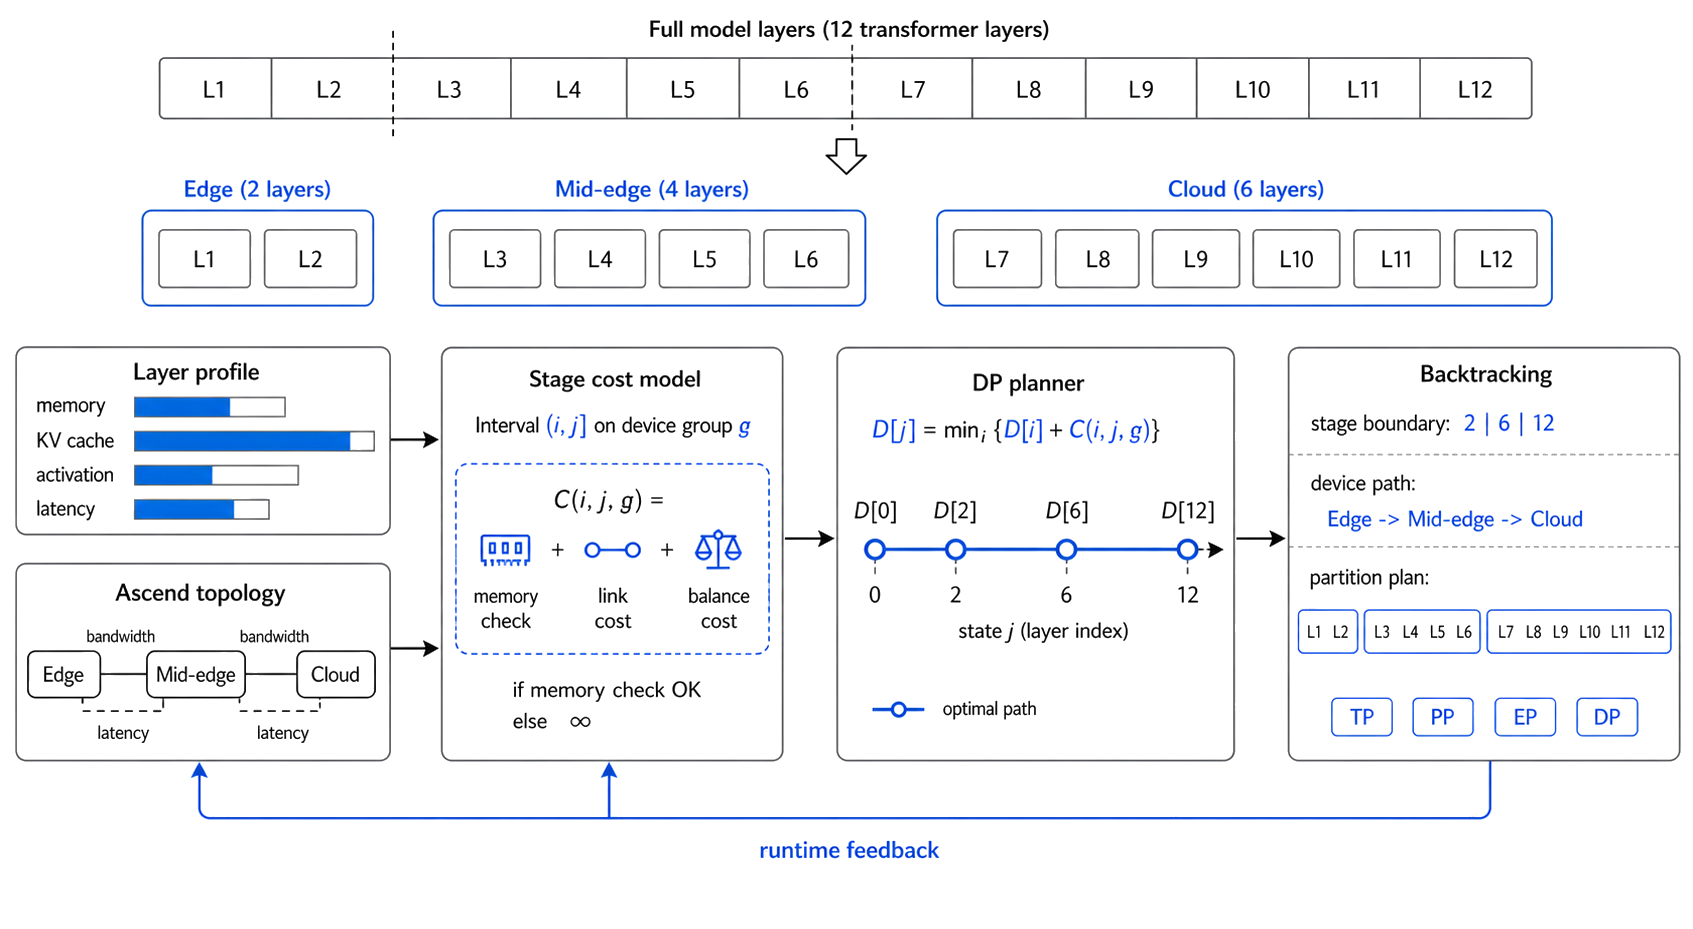
\includegraphics[width=\textwidth]{figures/ch4_dp_partition_architecture.png}
\caption{基于动态规划的层级切分部署策略生成流程}
\label{fig:ch4-dp-partition-architecture}
\end{figure}

如图~\ref{fig:ch4-dp-partition-architecture} 所示，层级切分策略由 layer profile、Ascend topology、stage cost model 和 DP planner 共同生成。为了避免把“切分方案”写成一个过于抽象的黑盒，第四章的决策变量可以明确写成
\[
x=\{K,\{l_k,g_k,e_k\}_{k=1}^{K}\}.
\]
其中，\(K\) 表示模型被切成多少个连续 stage；\(l_k\) 表示第 \(k\) 个 stage 的右边界，因此第 \(k\) 个 stage 覆盖 layer 区间 \((l_{k-1},l_k]\)，且 \(l_0=0,l_K=N\)；\(g_k\) 表示该 stage 放置到哪个 Ascend 设备组或节点组；\(e_k\) 表示该 stage 在当前 runtime 已支持范围内启用的执行能力，例如单设备执行、TP、PP+TP、EP、KV/offload 或阶段间状态传输。这样，第四章真正要决策的是“切在哪里、每段放哪里、每段用什么已支持执行能力”，而不是在几类并行方法之间做人工选择。

在论文建模上，可以把问题写成从安全可部署取值空间中选择低代价层级切分方案：
\[
\begin{array}{l}
x^\star=\arg\min\limits_{x \in \mathcal{X}_{\mathrm{safe}}} J(x),\\
J(x)=
w_t T(x)+w_c C(x)+w_m M(x)+w_b B(x)-w_g G(x).
\end{array}
\]
其中，\(\mathcal{X}_{\mathrm{safe}}\) 表示经过 runtime 支持检查、资源检查和 SLA 检查后的安全取值空间。\(T(x)\) 表示 TTFT、TPOT、E2E latency 和 pipeline bubble 等时延代价；\(C(x)\) 表示 activation/hidden state、KV 或 stage 交接带来的通信代价；\(M(x)\) 表示显存水位、runtime reserve 和 OOM 风险；\(B(x)\) 表示 stage 执行时间不均衡造成的流水线阻塞；\(G(x)\) 表示满足 SLA 的有效吞吐收益。这个目标函数不需要展开到每个 kernel，而是服务于验证环境中的部署决策：在不违反显存、链路和 SLA 约束的前提下，选择总代价更低、有效吞吐更高的层级切分方案。

这些决策变量的取值由系统自动生成。首先，规划器根据模型 layer 数和 layer profile 生成所有连续区间 \((i,j]\)，并用前缀和快速得到该区间的权重、activation 峰值、KV 增量和 prefill/decode 计算量。其次，根据 Ascend topology 生成可承载 stage 的设备组 \(g\)：单卡、同机多卡、跨节点设备组或端-边-云层级组合都要带有可用算力、可用显存、链路带宽和 RTT 信息。再次，runtime capability 决定 \(e_k\) 的取值：如果连续 layer stage 加载和跨设备 hidden state 传输可用，则允许层级 stage；如果 TP collective 可用且链路代价可接受，则允许该 stage 使用 TP；如果模型包含 MoE expert 且 runtime 支持 expert 驻留或换入，则允许 EP；如果 KV/offload 或阶段间状态传输已经被 runtime 支撑，也可以作为该 stage 的执行能力进入评估。未通过能力检查或资源检查的取值不会进入后续 DP 递推。

动态规划负责在这些可执行取值中生成最终层级切分策略。规划器先计算把连续区间 \((i,j]\) 放到设备组 \(g\) 上的 stage cost \(C(i,j,g)\)。这里的 \(C(i,j,g)\) 与图~\ref{fig:ch4-dp-partition-architecture} 中的写法一致，是一个经过能力检查后的综合代价：它内部会在 \(\mathcal{E}_{\mathrm{ok}}(i,j,g)\) 中选择可用执行方式 \(e\)，并同时计入执行时间、显存水位、同步/传输代价和 pipeline balance。图中 Edge、Mid-edge 和 Cloud 承载不同数量的连续 layer，表示 DP 输出的不是平均切分，而是受设备算力、显存和链路代价共同约束的不均匀层级分配。若某个区间超过显存预算、链路预算或 SLA 风险阈值，则该取值直接被丢弃。对保留下来的可执行取值，DP 按 layer 顺序递推，记录到达每个 block 位置的最小代价和前驱切点。若记 \(D[j]\) 为完成前 \(j\) 个 block 的最小综合代价，则可简化写成
\[
D[j]=
\min_{i<j,\ g \in \mathcal{G}_{\mathrm{ok}}}
\left\{
D[i]
+C(i,j,g)
\right\},
\]
其中，\(\mathcal{G}_{\mathrm{ok}}\) 表示当前可用于承载 stage 的设备组。若需要展开 \(C(i,j,g)\)，它可以理解为 profiling 得到的 stage 执行代价、由 activation/hidden state 大小和链路状态估计的传输代价、显存检查代价以及 pipeline balance 惩罚的加权和；\(\mathcal{E}_{\mathrm{ok}}(i,j,g)\) 表示该区间在该设备组上已通过能力和资源检查的执行方式。递推完成后，系统从最后一个 block 反向回溯前驱切点，得到完整的 stage boundary 序列；再把每个 stage 对应的设备组和执行能力写入部署计划。这样，DP 不是抽象地给出一个分数最低的方案，而是实际生成“第几层到第几层放在哪个设备组、每段采用什么已支持执行方式、失败时回退到哪条路径”的部署策略。

在线阶段不应频繁重切模型。系统可以在 P99 TTFT 超标、显存水位接近阈值、链路退化、请求长度分布明显变化或 runtime capability 发生变化时触发重规划；新方案只有在预估收益超过阈值且安全检查通过后才执行，否则保持当前部署或回退到固定 PP/TP、单节点部署、平均层级切分等基线。最终的分割策略可按“先层级、再并行、后扩展”的顺序组织：先用动态规划确定 layer-wise stage boundary、stage placement 和 pipeline balance；再在具体 stage 上按 runtime 支持情况启用 TP、EP、DP replica 或 KV 迁移等能力；最后把 PD disaggregation、KV Cache Pool、semantic/token-level collaboration 等作为扩展能力纳入验证。这样既避免把方案写成空泛的人工选择，也能把第四章落到可测试、可对比、可部署的华为验证路径上。
\phantomsection
\subsection*{4.7 小结}
\addcontentsline{toc}{subsection}{4.7 小结}

本章围绕“一次推理中首先被切分的对象”组织 CEC 下的资源自适应模型切分部署方法。Layer-wise / Vertical Partitioning 关注 layer、block 或 model shard 如何跨节点展开；Tensor / Operator-level Partitioning 关注同一层内部的 tensor、head、MLP 或通信 primitive 如何并行；Expert / Component-level Partitioning 关注 MoE expert 等组件如何驻留、换入和跨层级访问；Inference Phase Partitioning 关注 prefill、decode、verification、download 等阶段如何匹配异构资源；Semantic / Token-level Partitioning 则关注 draft、verify、semantic segment 或 token-wise responsibility 等生成职责如何拆分。这个分类强调的是系统优化对象，而不是论文使用的术语本身。

这五类方法之间存在明显的互补关系。层级切分和张量/算子级切分主要解决模型容量、显存和并行度问题；专家/组件级切分更适合 MoE 等具有稀疏激活结构的模型；阶段切分用于缓解 prefill 与 decode 之间的资源画像差异；语义/token 级切分则把协同推理推进到生成过程内部。CEC 场景下的关键不在于选择某一种“万能切分”，而在于根据模型结构、节点能力、链路状态、KV 位置、业务 SLA 和隐私边界选择合适的切分粒度。

从工程落地看，资源自适应切分不宜完全依赖一次性离线规划。离线 profiling 可以建立 layer cost、tensor cost、activation size、KV 增长和设备吞吐基线，并与 runtime capability 一起形成能力门控和代价估计；在线阶段仍需要根据负载、链路和请求长度修正这些代价。更稳妥的路线是“离线 profiling + 能力门控 + 事件触发动态规划重算 + 安全回退”：先判断 Ascend 推理栈在当前硬件拓扑上支持哪些切分和并行能力，再由动态规划搜索满足约束的低成本层级切分方案，最后通过收益阈值、冷却时间和回退路径避免频繁重配置。

结合本报告面向的验证环境，第四章的主线应放在以 Layer-wise / Vertical Partitioning 为基础的能力门控动态规划算法上。Layer-wise stage boundary、stage placement 和 pipeline balance 是主决策；tensor/operator-level、phase partitioning 和 expert/component-level 等方法不再作为人工挑选的“大方法”，而是映射到 vLLM-Ascend / MindIE 或 CANN 生态可支持、可压测、可回退的执行能力，例如 TP、PP、PP+TP、EP、layer sharding、context parallel、PD 分离、KV pool/offload 和 speculative decoding。Expert/component-level 与 semantic/token-level 方法适合作为扩展能力：前者用于 MoE 或组件化模型，后者适合端侧小模型可用且质量回退机制成熟的场景。这样既能覆盖研究前沿，也能将综述结论自然转化为可测试、可对比、可部署的算法方案。

\clearpage
\phantomsection
\section*{五、CEC 下的业务感知 Batching 参数优化方法}
\addcontentsline{toc}{section}{五、CEC 下的业务感知 Batching 参数优化方法}

LLM serving 中的 batching 不再只是传统 DNN 推理里的固定 batch size 选择。一次 LLM 请求通常先经历 prefill，再进入逐 token decode；请求到达时间、prompt 长度、输出长度、SLO、KV Cache 占用和上下文复用机会都会随时间变化。因此，batching 的核心问题可以定义为：在给定请求队列、实例负载、KV 状态和协作节点间链路条件下，动态决定哪些请求进入 batch、batch 在什么粒度更新、prefill 与 decode 是否混合、长 prompt 是否切块、不同阶段是否解耦，从而在 TTFT、ITL、TPOT、E2E latency、throughput、goodput 和资源利用率之间取得平衡。Orca 将生成式 Transformer serving 的调度粒度推进到 iteration level \cite{yu2022orca}；vLLM 通过 PagedAttention 为 continuous batching 提供了 KV 内存管理基础 \cite{kwon2023efficient}；Sarathi-Serve 代表 chunked prefill 路线 \cite{agrawal2024taming}，DistServe 则代表 prefill/decode disaggregation 路线 \cite{zhong2024distserve}。
在 CEC 场景中，这个问题进一步复杂化。单个请求入口附近的节点或服务实例通常只有较小的请求池，单纯等待大 batch 会破坏 TTFT；边缘 GPU/NPU 显存有限，KV Cache 会限制可并发 decode 请求数；终端接入链路和边缘节点间链路状态会影响 prefill offloading、decode placement 和状态传输收益；不同业务还可能具有差异化 SLO，例如机器人控制、车联网辅助决策、工业现场问答和普通对话服务的最大等待时间并不相同。基于这些特点，本章以 batching 机制及 batch 更新粒度为分类主线，并将 SLO、KV Cache、多租户和推测验证等因素作为贯穿各类方法的调度约束。
这些横向因素分别影响请求接纳、batch 组成、KV 管理和执行顺序。例如，SOLA/JITServe 根据 SLO 约束控制请求接纳，vLLM 为 KV-aware continuous batching 提供内存管理基础，S-LoRA/Punica 中的多租户 adapter serving 会改变 batch 的组成方式和执行算子，AdaServe 和 MuxServe 则分别引入推测验证与多模型时空复用条件下的批处理决策。
本文将 CEC 下的业务感知 batching 参数优化划分为四类：
\begin{enumerate}
\item \textbf{Queue-level Dynamic / Admission Batching}：batch 在请求进入执行前根据到达情况、等待窗口、优先级、距离 deadline 的剩余时间或 admission threshold 动态组成。
\item \textbf{Continuous Batching / Iteration-level Batching}：以 decode iteration 或 token iteration 为边界动态维护 active batch，使完成请求退出、新请求或被抢占请求加入。
\item \textbf{Chunked Prefill / Blended Batching}：把长 prefill 切成 chunk，并与 decode token 或其他请求混合执行，缓解长 prompt 对 decode 的阻塞。
\item \textbf{Disaggregated Prefill-Decode Batching}：将 prefill 和 decode 分配给不同实例、资源池或协作节点，分别形成阶段 batch，并通过 KV/state transfer 衔接。
\end{enumerate}

这四类方法从 batch 的形成与更新粒度描述不同的批处理组织方式，彼此之间可以组合使用。本文以固定参数、按到达顺序形成批次的 Static-FIFO 作为实验基线；四类主体方法则分别面向请求接纳与动态组批、迭代级 active batch、prefill chunk 混合和 prefill/decode 阶段解耦。Queue-level dynamic/admission batching 可以引入 SLO-aware priority；Continuous batching 可以结合抢占、KV-aware admission 和 active set 调整，Orca~\cite{yu2022orca} 和 FastServe~\cite{wu2026fastserve} 分别体现了 iteration-level scheduling 与 preemptive scheduling 的代表路线；Chunked Prefill / Blended Batching 通常建立在 continuous batching runtime 之上，Sarathi-Serve~\cite{agrawal2024taming} 是这一方向的典型系统；Disaggregated Prefill-Decode Batching 则将两个阶段的 batch 分配到不同资源池，DistServe~\cite{zhong2024distserve} 是阶段解耦路线的代表。

表~\ref{tab:cec-batching-overview} 汇总了与 batching 执行机制直接相关的代表工作以及会改变批处理决策的横向机制；图~\ref{fig:cec-batching-taxonomy} 给出了四类方法在批次形成粒度上的分类主线。SLO-aware、multi-tenant、KV-aware、speculative verification、multi-model serving 和 inference/finetuning co-serving 贯穿上述分类，并通过请求优先级、batch 组成、显存占用和资源竞争影响调度结果。LoRA serving、多模型 serving 和 inference/finetuning co-serving 的关键问题在于，如何组织不同 adapter、模型或任务类型共享 batch 与 GPU 时间片，并在 SLO、显存和阶段干扰约束下确定执行顺序，因此也被纳入比较。

\begingroup
\scriptsize
\setlength{\tabcolsep}{1.4pt}
\renewcommand{\arraystretch}{1.35}
\emergencystretch=2em
\begin{longtable}{@{}>{\raggedright\arraybackslash\hspace{0pt}}p{0.035\textwidth} >{\raggedright\arraybackslash\hspace{0pt}}p{0.175\textwidth} >{\raggedright\arraybackslash\hspace{0pt}}p{0.095\textwidth} >{\raggedright\arraybackslash\hspace{0pt}}p{0.170\textwidth} >{\raggedright\arraybackslash\hspace{0pt}}p{0.155\textwidth} >{\raggedright\arraybackslash\hspace{0pt}}p{0.330\textwidth}@{}}
\caption{\textbf{CEC 下业务感知 Batching 参数优化方法相关工作}}
\label{tab:cec-batching-overview}\\
\toprule
\textbf{序号} & \textbf{代表工作} & \textbf{发表在哪} & \textbf{主归属} & \textbf{相关机制} & \textbf{方法关键词} \\
\midrule
1 & JITServe \cite{zhang2026jitserve} & NSDI 2026 & Queue-level Dynamic / Admission Batching & SLO-aware request admission & 根据请求 SLO deadline、剩余时间预算和当前服务带宽动态决定接纳、排序和组批 \\
\tabrowrule
2 & SOLA \cite{hong2025sola} & MLSys 2025 & Queue-level Dynamic / Admission Batching & SLO-aware scheduling；phase-aware scheduling & 根据成本模型预测 TTFT/TPOT 相对 SLO 的紧迫程度，对等待请求排序并决定谁优先进入 batch \\
\tabrowrule
3 & QLM \cite{jhaone} & AIOps@\newline ASPLOS 2024 & Queue-level Dynamic / Admission Batching & Queue management & 以满足端到端延迟 SLO 为目标，通过队列控制减少 head-of-line blocking 并提高 SLO attainment \\
\tabrowrule
4 & TimelyLLM \cite{ling2024timelyllm} & MobiSys 2026 & Queue-level Dynamic / Admission Batching & time utility；iteration-level control & 面向时间敏感应用，将 deadline 和 time utility 纳入 batch 接纳与请求优先级 \\
\tabrowrule
5 & Preble \cite{srivatsa2025preble} & ICLR 2025 & Queue-level Dynamic / Admission Batching & KV-aware admission；distributed prompt scheduling & 在分布式 serving 中把 prefix/KV cache 命中和负载均衡共同纳入请求分配，使共享 prompt 请求更容易进入可复用状态的实例 \\
\tabrowrule
6 & Fairness in Serving Large Language Models \cite{sheng2024fairness} & OSDI 2024 & Queue-level Dynamic / Admission Batching；Continuous / Iteration-level Batching & multi-tenant fairness；VTC & 在 continuous batching 机制上引入 Virtual Token Counter，用已服务 token 成本调整调度顺序，减少租户之间的服务不公平 \\
\tabrowrule
7 & Orca \cite{yu2022orca} & OSDI 2022 & Continuous / Iteration-level Batching & selective batching & 提出 iteration-level scheduling，新请求在 decode iteration 边界加入，完成请求及时退出 active batch \\
\tabrowrule
8 & FastServe \cite{wu2026fastserve} & NSDI 2026 & Continuous / Iteration-level Batching & preemptive scheduling & 在 continuous batching 基础上引入迭代级抢占，缓解长请求占用和尾延迟问题 \\
\tabrowrule
9 & TokenFlow \cite{chen2026tokenflow} & EuroSys 2026 & Continuous / Iteration-level Batching & streaming token scheduling & 以 token stream / scheduling interval 为控制粒度，动态做 admission、preemption 和 resumption \\
\tabrowrule
10 & vLLM \cite{kwon2023efficient} & SOSP 2023 & Continuous / Iteration-level Batching & KV block memory management & PagedAttention 用逻辑/物理 KV block 映射降低显存碎片，为更大的 active batch 提供内存基础 \\
\tabrowrule
11 & SGLang \cite{zheng2024sglang} & NeurIPS 2024 & Continuous / Iteration-level Batching & RadixAttention；prefix reuse & 通过 RadixAttention 自动匹配和复用共享前缀 KV，使复杂多轮、RAG 和 agent workload 的 active batch 更少重复 prefill \\
\tabrowrule
12 & Llumnix \cite{sun2024llumnix} & OSDI 2024 & Continuous / Iteration-level Batching & runtime rescheduling；live migration & 在多个 vLLM 实例之间迁移运行中请求及其内存状态，缓解 active batch 负载不均、优先级变化和尾延迟问题 \\
\tabrowrule
13 & Punica \cite{chen2024punica} & MLSys 2024 & Continuous / Iteration-level Batching & multi-tenant LoRA batching & 用 SGMV 等算子支持不同 LoRA adapter 请求共享同一基础模型 batch，降低多租户 LoRA serving 的显存和计算浪费 \\
\tabrowrule
14 & S-LoRA \cite{sheng2024slora} & MLSys 2024 & Continuous / Iteration-level Batching & heterogeneous adapter batching；unified paging & 通过统一分页管理 adapter 权重和 KV cache，并用定制 LoRA 算子支持大量 adapter 请求在同一 serving 实例中批处理 \\
\tabrowrule
15 & NanoFlow \cite{zhu2025nanoflow} & OSDI 2025 & Continuous / Iteration-level Batching；Chunked Prefill / Blended Batching & nano-batch scheduling & 将执行拆成 nano-batches 并搜索数量、大小和顺序，同时对长 prefill 做 token 粒度分块 \\
\tabrowrule
16 & Sarathi-Serve \cite{agrawal2024taming} & OSDI 2024 & Chunked Prefill / Blended Batching & chunked prefill；decode interleaving & 将长 prefill 切成 chunk，并与 decode 混合交错执行，平滑两阶段负载 \\
\tabrowrule
17 & Libra \cite{ruan2026libra} & NSDI 2026 & Chunked Prefill / Blended Batching & phase quota control & 在混合批次中调控 prefill 与 decode token 配额比例，降低两阶段算子干扰 \\
\tabrowrule
18 & A Hybrid Online and Offline Requests Inference Serving System for LLM in Private Computer Environment \cite{shen2025hybrid} & IEEE TC 2026 & Chunked Prefill / Blended Batching & online/offline mixed batching & 在同一 continuous batch 内组织在线 prefill/decode 与离线任务，在线优先、离线填充空闲资源 \\
\tabrowrule
19 & LLMStation \cite{he2025resource} & USENIX ATC 2025 & Chunked Prefill / Blended Batching & iteration-level multitasking；inference/tuning co-serving & 将 fine-tuning 任务改造成可挂起流水线，并在 iteration 粒度批处理 inference 与 tuning 请求，以提高 GPU 利用率同时满足 serving SLO \\
\tabrowrule
20 & FlexLLM \cite{oliaro2026flexllm} & NSDI 2026 & Chunked Prefill / Blended Batching & token-level co-serving；SLO-aware scheduling & 将 inference 和 PEFT finetuning 融合到 token 级执行，并优先保护 latency-sensitive inference 的 SLO，再利用空闲 token 预算推进 finetuning \\
\tabrowrule
21 & AdaServe \cite{li2026adaserve} & EuroSys 2026 & 横向机制：Speculative Verification Batching & multi-SLO speculative decoding & 按请求 SLO 定制 speculation tree，并通过 speculate-select-verify pipeline 形成验证批处理；它主要补充 multi-SLO 场景下的验证调度，而不是 prefill chunking \\
\tabrowrule
22 & DistServe \cite{zhong2024distserve} & OSDI 2024 & Disaggregated Prefill-Decode Batching & phase-specific workers & 将 compute-heavy prefill 与 memory/latency-sensitive decode 解耦到不同 worker pool \\
\tabrowrule
23 & Splitwise \cite{patel2024splitwise} & ISCA 2024 & Disaggregated Prefill-Decode Batching & prompt pool；token pool & 将 prompt computation 和 token generation 放到不同机器池，并分别匹配硬件资源 \\
\tabrowrule
24 & Mooncake \cite{qin2025mooncake} & USENIX FAST 2025 & Disaggregated Prefill-Decode Batching & distributed KV cache；global scheduling & 在 prefill/decode 解耦基础上构建分布式 KVCache，并按 KV 本地性和 SLO 调度实例 \\
\tabrowrule
25 & MuxServe \cite{duan2024muxserve} & ICML 2024 & 横向机制：Multi-model Multiplexed Batching & adaptive batch scheduling；spatial-temporal multiplexing & 面向多 LLM serving 联合做空间共置和时间复用，并利用 prefill/decode 阶段特征设计 adaptive batch scheduling，以提升多模型场景下的 SLO 吞吐 \\
\bottomrule
\end{longtable}
\endgroup

\begin{figure}[!htbp]
\centering
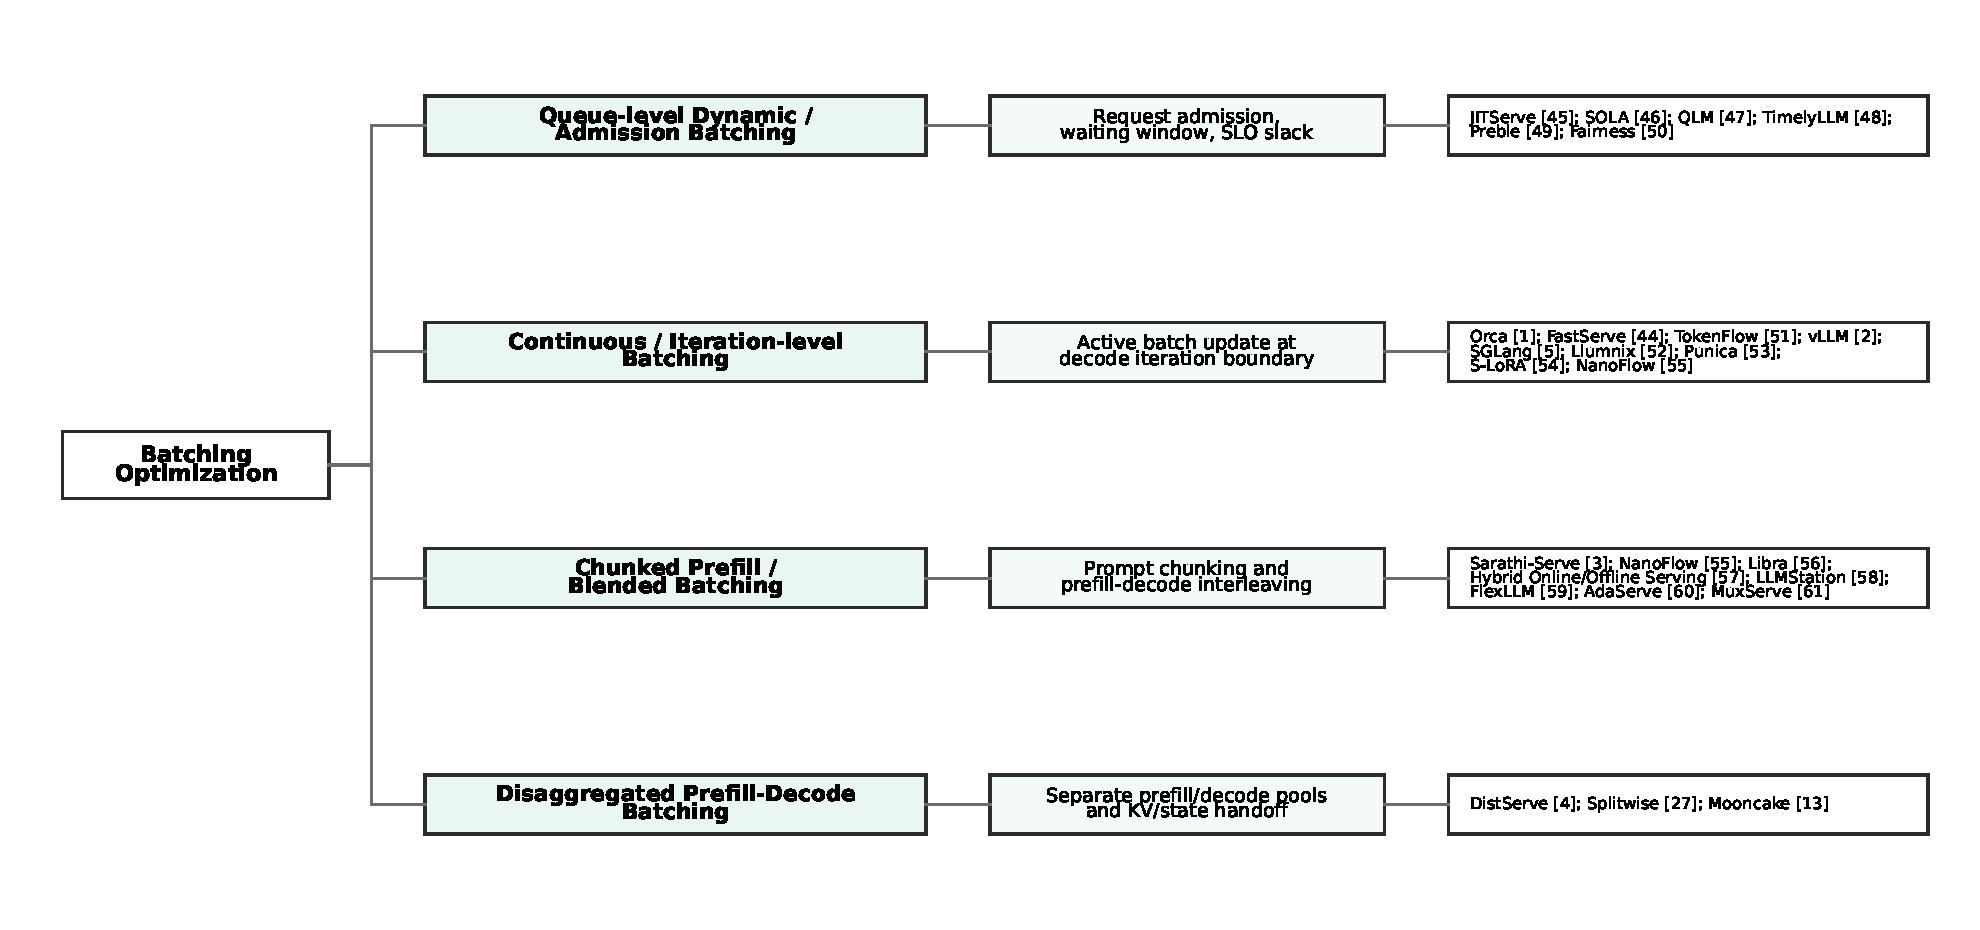
\includegraphics[width=\textwidth]{figures/ch5_batching_taxonomy.pdf}
\caption{\textbf{CEC 下业务感知 Batching 参数优化方法的分类树}}
\label{fig:cec-batching-taxonomy}
\end{figure}

\phantomsection
\subsection*{5.1 Queue-level Dynamic / Admission Batching}
\addcontentsline{toc}{subsection}{5.1 Queue-level Dynamic / Admission Batching}
Queue-level Dynamic / Admission Batching 要解决的是“固定等待固定 batch size 过于僵硬”的问题。真实 LLM 服务中，请求到达是随机的，prompt 长度、输出长度和 SLO 也不一致。如果系统仍按固定 batch size 或固定时间窗口组批，低负载时会等待过久，高负载时又可能把紧急请求排在队尾。因此，这类方法在请求进入执行前动态决定 batching window、batch membership、admission threshold 和请求优先级。JITServe 从 SLO-aware serving 角度建模请求服务带宽 \cite{zhang2026jitserve}，SOLA 以 state-aware scheduling 提高 SLO attainment \cite{hong2025sola}，QLM 关注队列管理和 head-of-line blocking \cite{jhaone}，TimelyLLM 则面向时间敏感机器人应用组织请求调度 \cite{ling2024timelyllm}。Preble 说明 prefix/KV locality 会改变请求分配 \cite{srivatsa2025preble}；Fairness in Serving Large Language Models 则说明多租户公平性也会改变请求排序和 token 服务顺序 \cite{sheng2024fairness}。

这种队列级决策可以抽象成图~\ref{fig:ch5-dynamic-admission-batching} 中的闭环：请求先等待，控制器再根据剩余时间预算决定立即执行还是继续合批。
\begin{figure}[!htbp]
\centering
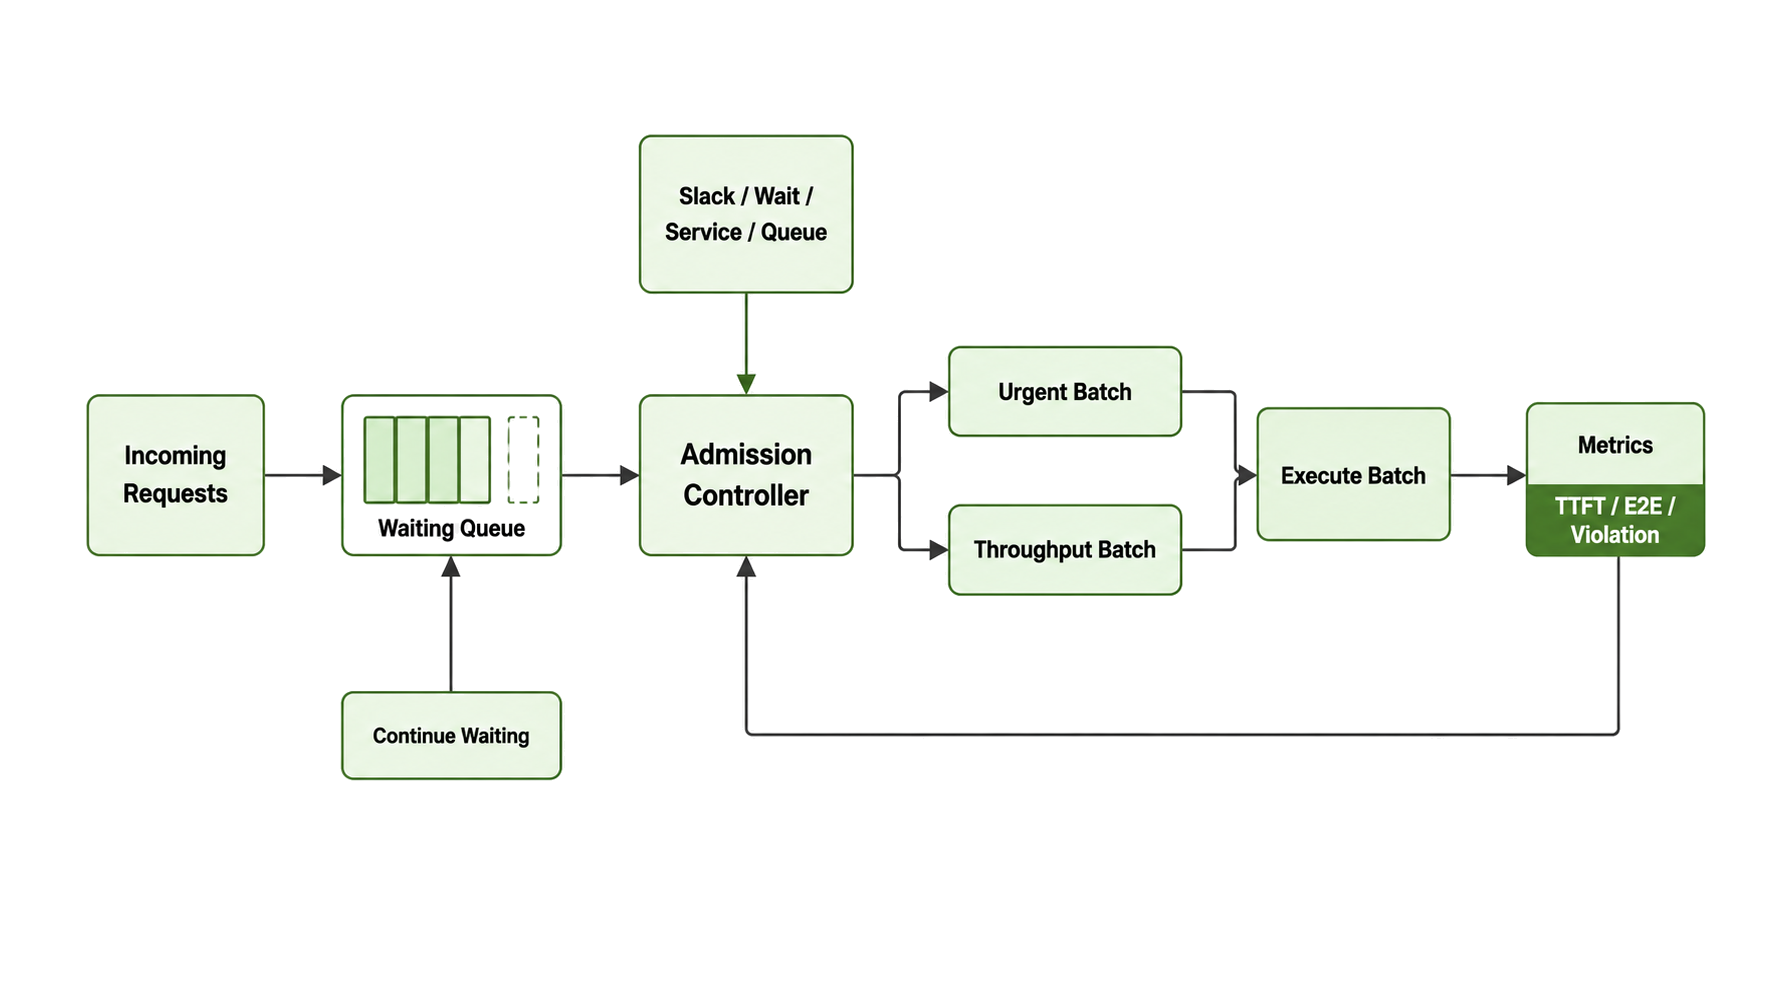
\includegraphics[width=\textwidth]{figures/ch5_2_dynamic_admission_batching.png}
\caption{\textbf{Queue-level Dynamic / Admission Batching 机制示意图}}
\label{fig:ch5-dynamic-admission-batching}
\end{figure}
Incoming Requests 携带 SLO 和 priority 进入 Waiting Queue，Admission Controller 持续读取距离 deadline 的剩余时间、wait time、service estimate 和 queue length。临近 deadline 的请求进入 Urgent Batch，剩余时间较充足的请求进入 Throughput Batch 或继续等待；两个可执行 batch 随后进入 runtime。执行产生的 TTFT、E2E latency 和 SLO violation 由 Metrics 模块反馈给控制器，用于调整 batching window 与 admission threshold。Dynamic batching 会同时改变 batch size、请求组成和等待时间，并围绕各请求的剩余时间预算在线决策。

这类方法的核心思想是把组批从静态规则改为在线决策。调度器可以根据队列长度、请求等待时间、距离 deadline 的剩余时间、prompt 长度、预计输出长度、业务优先级和当前实例负载决定是否立即发起 batch，还是继续等待更多请求。对于剩余时间较充足的请求，可以适当等待以提高吞吐；对于即将违反 TTFT 或 deadline 的请求，应尽快进入执行队列。与 static batching 相比，dynamic batching 的 batch 仍然主要在执行前形成，但形成过程已经具备业务感知能力。

Queue-level Dynamic / Admission Batching 的关键变量包括 batching window、max wait time、admission threshold、request priority、距离 deadline 的剩余时间、estimated service time 和 batch size limit。很多 SLO-aware request batching 工作可以放在这一类中理解：它们并不一定改变 decode iteration 的 active batch 机制，而是先在请求队列和接纳阶段决定谁应该进入下一批执行 \cite{zhang2026jitserve}, \cite{hong2025sola}。

在 CEC 中，dynamic batching 需要把网络时延纳入剩余时间预算。靠近请求入口的实例通常 RTT 较低，但请求池较小；能够聚合多个入口的协作节点请求池更大，但转发距离和排队时间也可能增加。因此，同一个请求应在入口附近立即小批次执行，还是转发到其他协作节点等待更合适的 batch，取决于剩余 SLO、入口到实例链路、当前排队时间和模型能力。Dynamic batching 是 CEC 中自然的业务感知入口，因为它在请求尚未进入长期 decode 循环前就可以完成接纳、排序和路径选择。

Queue-level Dynamic / Admission Batching 的风险在于调度器需要可靠估计请求服务时间。如果输出长度预测错误、队列状态滞后或网络时延估计不准，batching window 和优先级选择可能反而放大尾延迟。因此，在 CEC 中应避免过长等待窗口，并将 admission control、优先级老化和 fallback 策略作为配套机制。
\phantomsection
\subsection*{5.2 Continuous Batching / Iteration-level Batching}
\addcontentsline{toc}{subsection}{5.2 Continuous Batching / Iteration-level Batching}
Continuous Batching 进一步打破了 batch 生命周期。它要解决的是 LLM decode 阶段中请求完成时间不同导致的空槽浪费问题。传统 static 或 dynamic batching 即使在执行前能组成合适 batch，一旦进入自回归 decode，短请求会先完成，长请求还在继续生成。如果 batch 在整个生成过程中固定不变，已完成请求留下的 slot 无法被新请求利用，新到请求也必须等待当前 batch 全部结束。Orca 首先系统化提出 iteration-level scheduling 和 selective batching，成为后续 continuous batching 系统的基础 \cite{yu2022orca}。

当调度边界从请求级下降到 decode iteration 后，batch 的含义就变成图~\ref{fig:ch5-continuous-batching} 中持续变化的 active set。
\begin{figure}[!htbp]
\centering
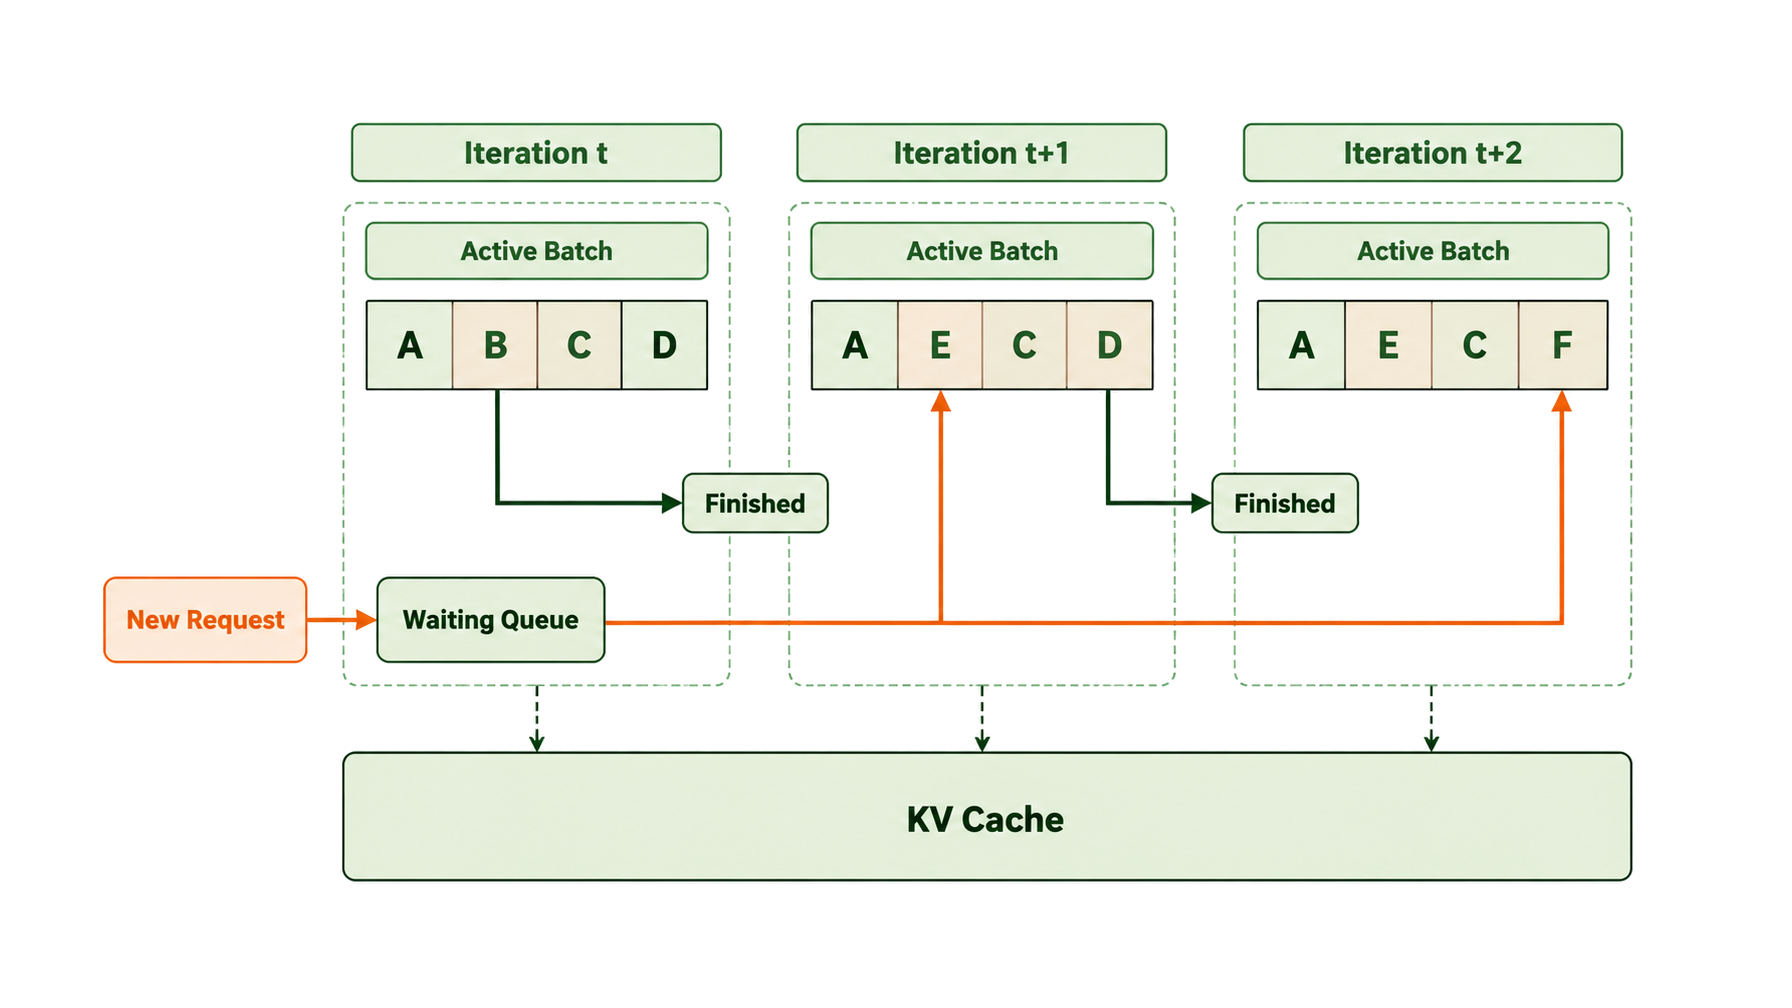
\includegraphics[width=\textwidth]{figures/ch5_3_continuous_iteration_batching.png}
\caption{\textbf{Continuous Batching / Iteration-level Batching 机制示意图}}
\label{fig:ch5-continuous-batching}
\end{figure}
图中每个 Iteration 表示一次 decode iteration，Active Batch 中的四个序列共同生成下一个 token。在 Iteration~\(t\) 结束后，请求 B 完成并退出，请求 E 从 Waiting Queue 加入，因此下一轮的 active set 由 A、B、C、D 变为 A、E、C、D；到 Iteration~\(t+1\) 结束后，请求 D 退出、请求 F 加入，active set 进一步变为 A、E、C、F。A 和 C 连续保留在三个迭代中，其 KV Cache 也持续增长。该过程说明，continuous batching 会在迭代边界及时回收完成请求留下的 slot，并用等待请求补充空位，而不必等待整个 batch 结束。

Continuous Batching 的解决思路，是把 batch 的更新边界缩短到 decode iteration。每生成一轮 token 后，系统都可以移除已经完成的请求，加入完成 prefill 的新请求，或者恢复被抢占的请求。这样 batch 不再是一组固定请求，而是一个随 token 生成持续变化的 active set。Orca 将这一思想形式化为 iteration-level scheduling，使 LLM serving 从“按完整请求批处理”转向“按 token iteration 批处理” \cite{yu2022orca}；FastServe 在这一基础上引入迭代级抢占 \cite{wu2026fastserve}，TokenFlow 面向 streaming token 服务做 preemptive scheduling \cite{chen2026tokenflow}，NanoFlow 则用 nano-batch execution 进一步细化执行流 \cite{zhu2025nanoflow}。

这类方法的核心变量包括 active sequence set、decode batch size、token iteration order、join policy、leave policy、preemption policy、resume policy 和 KV block allocation。由于每轮 decode 都要读取并追加 KV Cache，continuous batching 必须和内存管理绑定：请求能否加入 active batch，不仅取决于是否有计算 slot，也取决于是否有足够 KV block 和状态本地性。vLLM 的 PagedAttention 正是从 KV block 管理角度支撑更大的 active batch 和更低的显存碎片 \cite{kwon2023efficient}；SGLang 用 RadixAttention 复用共享前缀 \cite{zheng2024sglang}；Llumnix 则把运行中请求迁移纳入多实例调度 \cite{sun2024llumnix}。这些工作说明，continuous batching 的 active set 会进一步受到 prefix cache 和实例负载的共同约束。

多租户 LoRA serving 也可以从 continuous batching 角度理解。Punica~\cite{chen2024punica} 和 S-LoRA~\cite{sheng2024slora} 让使用不同 adapter 的序列共享同一个基础模型执行批次，并处理 adapter 权重分页、异构 adapter batching 和定制 LoRA 算子等问题。这些机制决定 batch 内请求能否合并执行，以及合并后的显存和算子开销。

在 CEC 中，Continuous Batching 不能简单照搬云端大请求池策略。靠近请求入口的边缘实例并发通常较低，短时间内能加入 active batch 的请求有限；如果为等待更多 token stream 而延长调度周期，TTFT 会恶化。因此，局部实例更适合短窗口、低等待的 micro-continuous batching，能够聚合多个入口的协作节点则可以形成更稳定的 active batch。对于移动用户，还需要考虑请求是否会在 decode 期间切换入口，避免 active batch 中的 KV 状态和用户路径频繁迁移。

Continuous Batching 是现代 LLM serving 的基础能力，但不是完整的业务感知调度。它提升 decode 阶段资源利用率，却不天然感知 SLO、应用等级、KV 状态迁移、边缘链路和隐私约束。因此，在 CEC 中应把 Continuous Batching 视为 runtime 基座，再叠加 dynamic priority、phase-aware interleaving 和状态感知 admission。
\phantomsection
\subsection*{5.3 Chunked Prefill / Blended Batching}
\addcontentsline{toc}{subsection}{5.3 Chunked Prefill / Blended Batching}
Chunked Prefill / Blended Batching 要解决的是长 prefill 阻塞 decode 的问题。Prefill 处理完整 prompt，矩阵规模大、并行度高，通常更偏 compute-bound；decode 逐 token 生成，频繁访问 KV Cache，更偏 memory-bound 或 latency-bound。如果长 prompt prefill 连续占用 GPU，已经在流式输出的请求会出现 ITL 抖动；如果完全优先 decode，新请求 TTFT 又会被推迟。两阶段混部需要确定 prefill 和 decode 在同一执行资源上的交错方式。Sarathi-Serve~\cite{agrawal2024taming} 将长 prefill 切成 chunks 并与 decode 交错，是这一类方法的代表性工作。

长 prompt 不能直接整段 prefill 的原因，可以通过图~\ref{fig:ch5-chunked-prefill-batching} 看到：系统需要把 prefill chunk 和 decode token 交错安排，在 TTFT 与 ITL 之间控制阶段干扰。
\begin{figure}[!htbp]
\centering
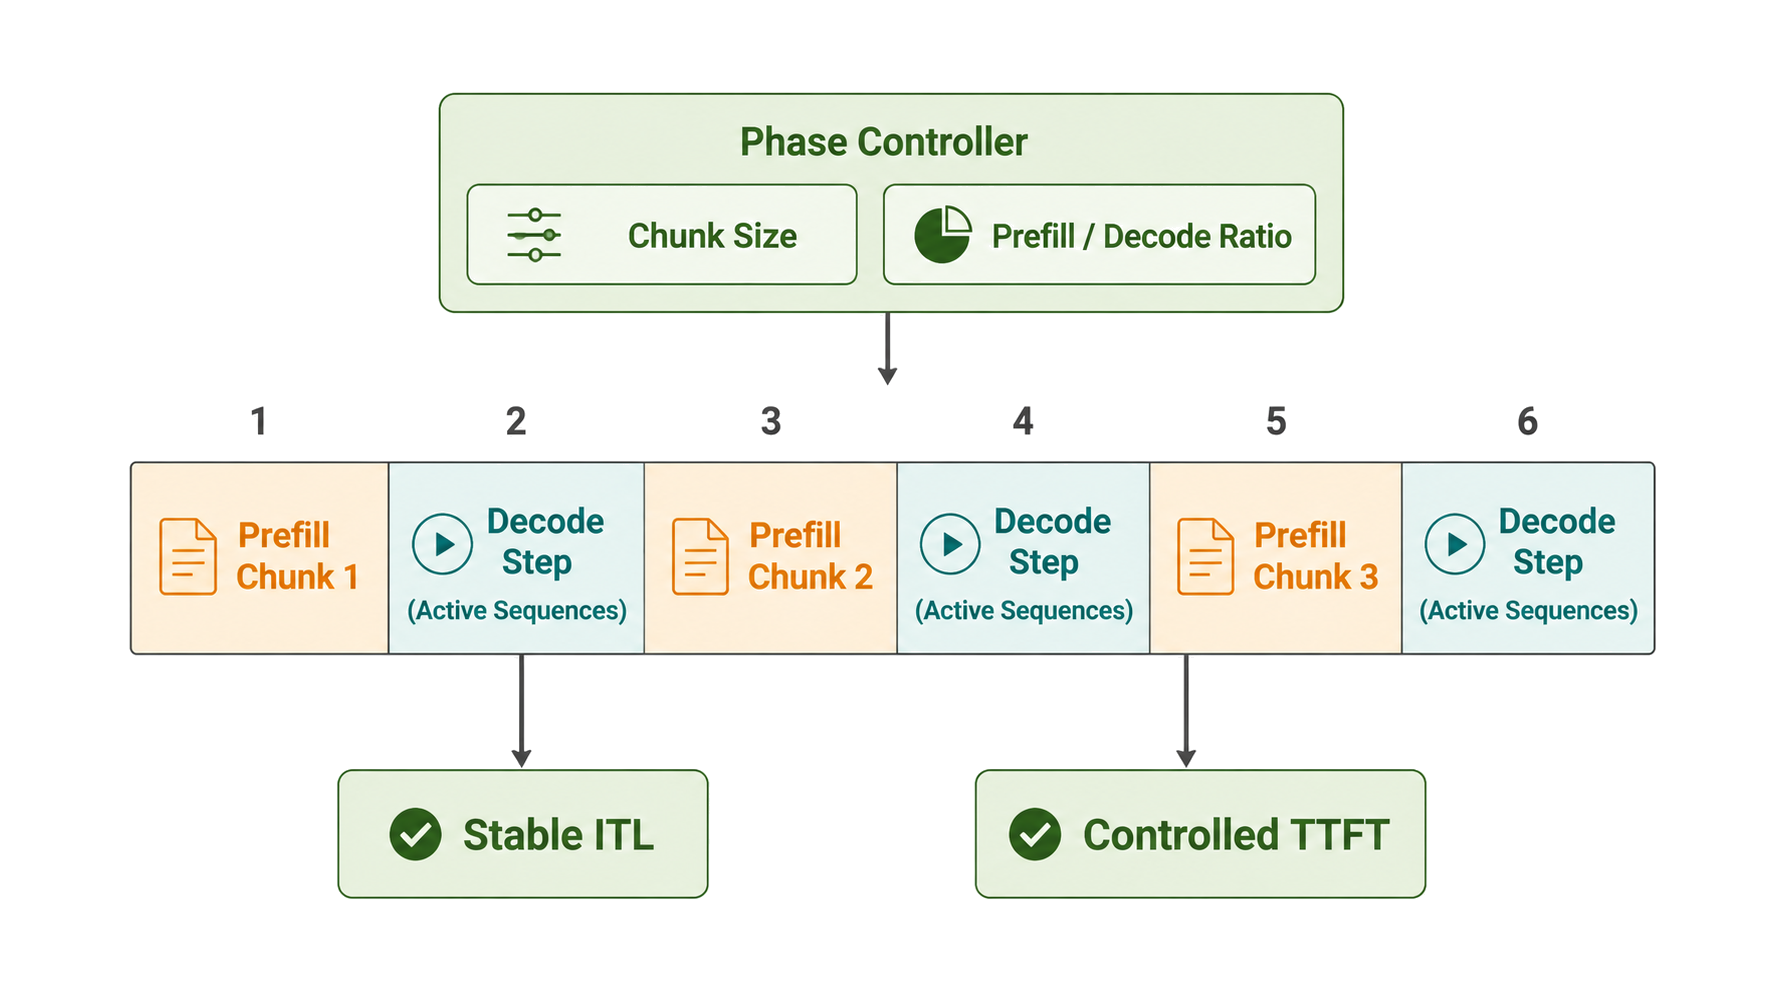
\includegraphics[width=\textwidth]{figures/ch5_4_chunked_prefill_blended_batching.png}
\caption{\textbf{Chunked Prefill / Blended Batching 机制示意图}}
\label{fig:ch5-chunked-prefill-batching}
\end{figure}
图中 Long Prompt 被拆成三个 prefill chunks，并与 Active Sequences 的 decode steps 交替进入六个连续的调度时隙。Phase Controller 通过 chunk size 和 prefill/decode ratio 控制每次执行的 prefill 工作量以及两类阶段的交错频率：chunk 较大时能够提高 prefill 效率，但可能拉长 decode 间隔；chunk 较小时更有利于稳定 ITL，却会增加调度和 kernel 启动开销。因此，该机制通过有限粒度的切块与交错，在保持 decode 流畅性的同时控制新请求的 TTFT。

Chunked Prefill 的思想是把长 prompt 拆成多个 prefill chunk，而不是一次性执行完整 prefill。Blended Batching 则进一步把 prefill chunk 与 decode token 混合在同一个调度周期或同一个 batch 中，使 compute-heavy 的 prefill 和 memory/latency-sensitive 的 decode 交错执行。这样可以平滑每轮计算量，减少长 prefill 对 decode 的阻塞，也能避免 decode 完全占用调度周期导致新请求 TTFT 过高。

这类方法的核心变量包括 chunk size、prefill token budget、decode token budget、prefill-to-decode ratio、interleaving policy、phase quota、online/offline mixing ratio 和 stall control。Chunk 太大，会重新造成 prefill 阻塞；chunk 太小，会增加调度和 kernel overhead。Prefill/decode 比例太偏向 prefill，会伤害 ITL；太偏向 decode，会伤害 TTFT。因此，Chunked Prefill / Blended Batching 的本质是阶段内混合调度和阶段间干扰控制。Libra 可以理解为阶段配额控制的扩展 \cite{ruan2026libra}，NanoFlow 代表更细粒度执行流优化 \cite{zhu2025nanoflow}，LLMStation 和 FlexLLM 则把混合对象扩展到 inference/finetuning co-serving 等更复杂 workload \cite{he2025resource}, \cite{oliaro2026flexllm}。这些工作本质上仍然需要在同一批执行资源上安排不同类型 token 或任务片段的执行顺序。MuxServe 同样涉及 batch scheduling，但其主问题是多模型 serving 的空间共置与时间复用，更适合作为 multi-model multiplexed batching 的横向机制，而不是 chunked prefill 的直接代表 \cite{duan2024muxserve}。

在 CEC 中，这类方法适合由不同能力的边缘节点协同执行。靠近请求入口的节点可以保持较短 decode 间隔，算力更强的协作节点处理较长 prefill chunk；当链路稳定且 KV 传输成本可控时，系统还可以把长 prompt prefill 分配到更强节点，再将可复用状态交给靠近用户的 decode 节点。若链路抖动大或边缘并发不足，过度切分 prefill 可能增加状态传输和调度开销，因此 chunk size 和 interleaving ratio 必须纳入在线代价模型。

Chunked Prefill / Blended Batching 比 continuous batching 更直接处理 prefill/decode 干扰。它适合长 prompt、多轮对话、RAG 增强上下文和流式输出并存的场景，但需要准确控制 chunk size 和阶段配额。对于 CEC，关键是把网络传输和 KV 状态位置纳入阶段混合决策，否则 prefill 拆得越细，跨节点状态交接越可能成为新的瓶颈。
\phantomsection
\subsection*{5.4 Disaggregated Prefill-Decode Batching}
\addcontentsline{toc}{subsection}{5.4 Disaggregated Prefill-Decode Batching}
Disaggregated Prefill-Decode Batching 是对 phase-aware 思路的进一步扩展。Chunked Prefill / Blended Batching 仍然假设 prefill 和 decode 在同一个实例或同一类资源上交错执行；而 disaggregated batching 直接把两阶段拆到不同 worker pool、不同 GPU 实例、不同机器池或不同协作边缘节点。Prefill batch 和 decode batch 分别形成，分别扩缩容，并通过 KV Cache 或中间状态传输衔接。DistServe 从 goodput 优化角度论证阶段解耦 \cite{zhong2024distserve}，Splitwise 强调 prompt pool 与 token pool 的硬件匹配 \cite{patel2024splitwise}，Mooncake 则在 prefill/decode 解耦基础上构建 KVCache-centric serving 架构 \cite{qin2025mooncake}。

PD 分离后的 batching 可以按图~\ref{fig:ch5-disaggregated-pd-batching} 理解：prefill instance 内部形成 prompt batch，decode instance 内部维护 active sequence batch，两个池之间通过 KV/state handoff 连接。
\begin{figure}[!htbp]
\centering
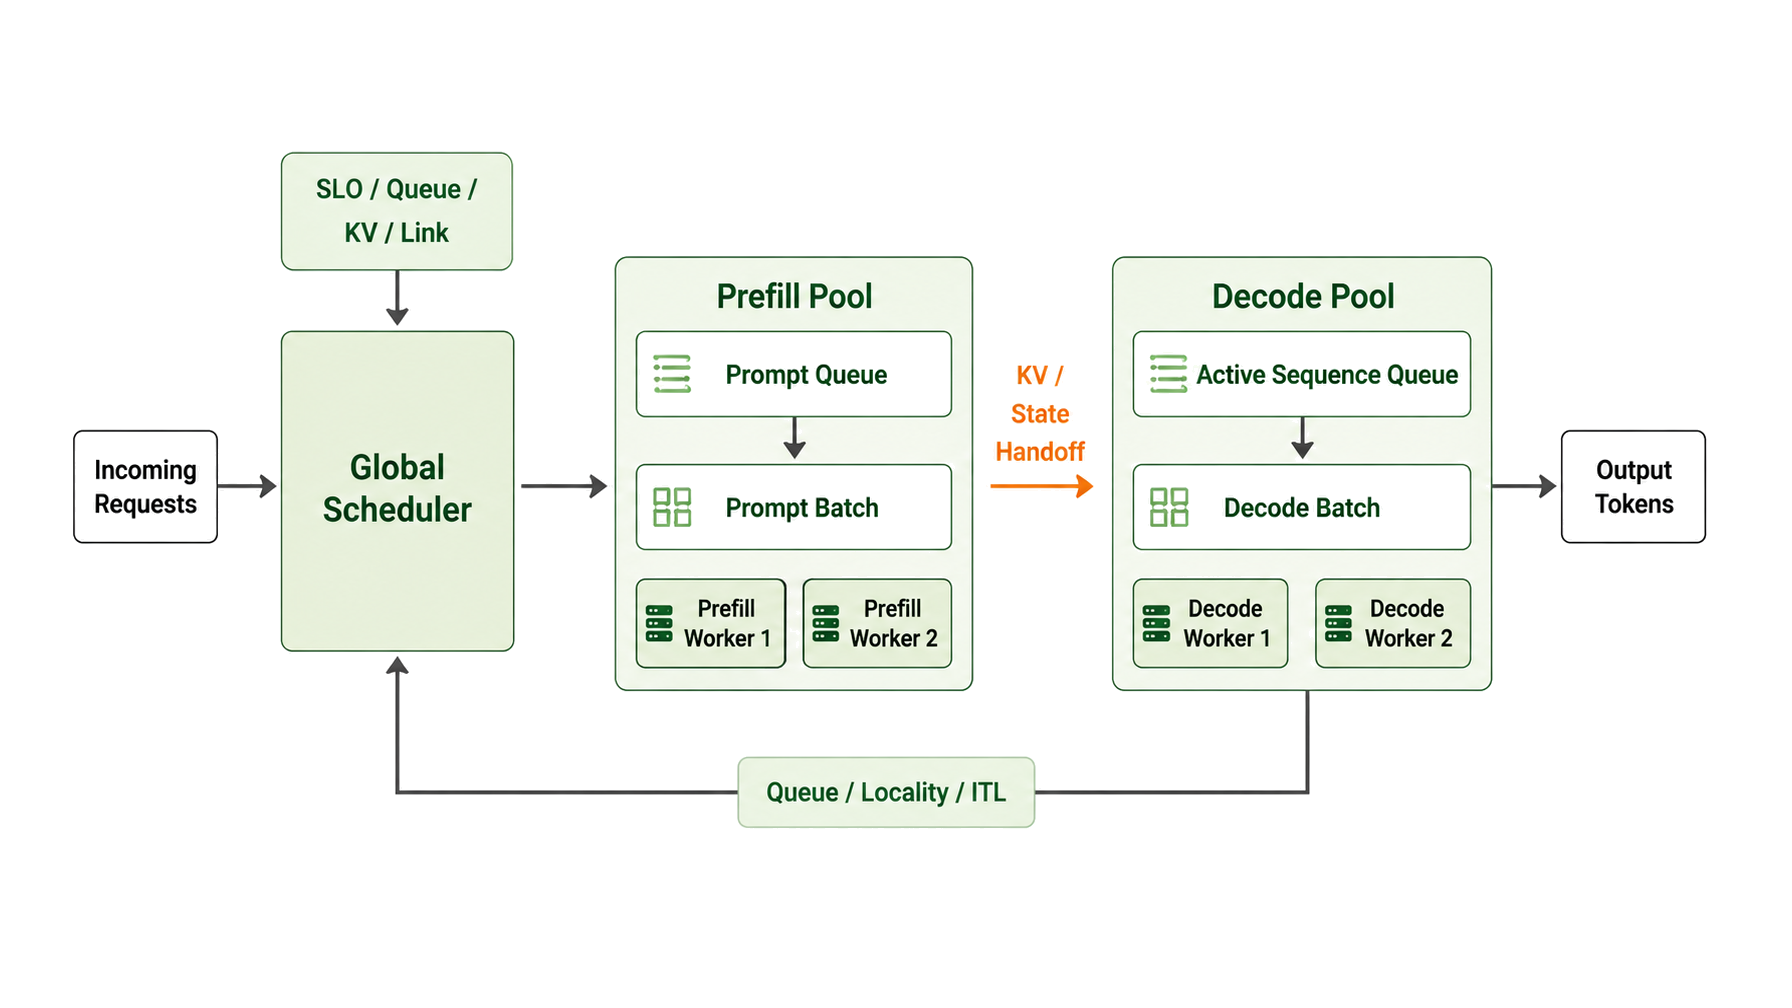
\includegraphics[width=\textwidth]{figures/ch5_5_disaggregated_pd_batching.png}
\caption{\textbf{Disaggregated Prefill-Decode Batching 机制示意图}}
\label{fig:ch5-disaggregated-pd-batching}
\end{figure}
Global Scheduler 根据 SLO、queue length、KV locality 和 link state 将请求送入 Prefill Pool；Prefill Worker 形成 prompt batches 并生成初始 KV blocks。随后 KV / State Handoff 将 KV blocks、state transfer 和 metadata 交给 Decode Pool，Decode Worker 再维护 active sequence batches 并输出 tokens。图中的反馈路径表示 queue length、KV locality、ITL 等运行时指标回流到全局调度器，用于调整后续请求进入哪个 pool 以及是否需要扩缩容。因此，PD 分离后的 batching 实际上变成两个 pool 的独立组批与跨池状态协调问题。

这类方法的出发点是 prefill 和 decode 的计算与访存特征明显不同。Prefill 更偏 compute-bound，适合吞吐导向、更强算力或更大 batch 的资源池；decode 更偏 memory/latency-bound，需要稳定 ITL、低排队和快速状态访问。若两者混部在同一资源池中，长 prefill 可能阻塞 decode，decode 小步迭代又可能降低 prefill 吞吐。Disaggregation 通过物理或逻辑隔离减少两阶段干扰，并允许系统分别为 prefill 和 decode 选择 parallelism、batch size 和扩缩容策略。

Disaggregated Prefill-Decode Batching 的核心变量包括 prefill worker pool、decode worker pool、phase queue、KV transfer、state locality、worker scaling、prefill/decode routing 和 global scheduling。它的收益来自阶段资源匹配和干扰隔离，但代价集中在 KV 传输、状态连续性和跨节点调度。Prefill 完成后，decode 必须访问初始 KV Cache；如果 KV 传输慢、远程访问不稳定或用户入口发生变化，disaggregation 的收益会被状态成本抵消 \cite{zhong2024distserve}, \cite{qin2025mooncake}。

本节关注 PD 分离之后的 batching：prefill pool 如何形成 prompt batch，decode pool 如何维护 active sequence batch，以及两个 pool 之间如何通过 KV/state handoff 协调。

在 CEC 中，disaggregated batching 可以映射到不同能力的协作节点：算力较强或能够聚合请求的节点承担 prefill-heavy 请求，靠近用户且持有会话状态的节点负责低时延 decode；容量较大的节点也可以维护 prefill pool 和 KV state service，其他节点只在需要较低 ITL 时承担 decode。对于移动用户，系统还需要判断 decode worker 是否应该跟随入口迁移，还是远程访问原有 KV。也就是说，CEC 下的 disaggregated batching 不能只看 GPU 利用率，还必须同时看链路稳定性、KV 迁移成本和服务连续性。

Disaggregated Prefill-Decode Batching 适合 prefill/decode 负载差异明显、阶段队列规模足够、状态传输成本可控的场景。若请求很短、边缘并发很低或链路抖动大，复杂阶段拆分可能不如本地 blended batching 稳定。因此，CEC 中应把 disaggregation 视为跨实例的资源组织方式，而不是默认打开的单点优化。
\phantomsection
\subsection*{5.5 面向华为验证环境的方案建议}
\addcontentsline{toc}{subsection}{5.5 面向华为验证环境的方案建议}

异构 Ascend 推理服务中的请求到达率、输入输出长度、KV Cache 占用和距离 deadline 的剩余时间不断变化，合适的 batch size、token budget、等待窗口和请求顺序也会随之改变。固定配置难以覆盖这些组合；普通强化学习虽然能够根据运行状态调整参数，但探索和随机输出可能造成显存越界、关键请求超时或运行时无法执行。为明确动态 batching 在不同请求特征下能够获得多大收益，本文先建立设备、网络、模型和请求的统一系统模型，分析请求长度与 batch size 变化时相对 Static-FIFO 的性能范围。该结果一方面刻画动态组批可利用的优化空间，另一方面为后续强化学习的状态、动作和优化目标设计提供依据。在此基础上，本文提出带拉格朗日约束和运行时安全投影的 Safe-RL batching 方法。

评价时先检查 SLA 和运行安全，再比较性能。对同一模型、请求轨迹和硬件环境，只有 P90/P99 TTFT、TPOT 和 E2E latency 满足业务配置，显存保持在可用范围内，且受控实验中未发生 OOM、不可执行动作和已接纳关键请求硬超时，该运行点才进入完成请求速率与平均 E2E latency 的比较。实验目标是相对 Static-FIFO 将满足 SLA 的请求处理速度提高 20\%，平均 E2E latency 下降 20\%，并保持零硬违规 \cite{huawei2026internal}。

为估计动态组批在验证环境中的性能空间，本文选取四卡 A800T-A2、100~Gbps 直连场景，CodeLlama34B 和 Qwen2-VL-7B-Instruct 沿用第四章得到的非均匀 PP 部署，并让输入和输出覆盖短、中、长三档。具体设备算力、layer 分配和请求长度设置将在后文给出。

理论分析中的 Static-FIFO 使用固定 batch size 和等待窗口，按请求到达顺序形成批次，并在当前批次完成后再处理下一批。批内输入按最长 prompt 补齐，生成过程持续到最长输出结束。极端情况下，一个 batch 包含 1 个最长请求和 63 个最短请求，短请求会承担大量额外计算。用 Static-FIFO 的总计算量除以所有请求各自所需计算量之和，再减 1，得到 \textbf{CodeLlama34B 和 Qwen2-VL-7B-Instruct 的计算侧提升上界分别为 1060.2\% 和 353.9\%}，该上界属于理论上界，实际部署中达不到。

为了在训练 Safe-RL 前先观察长度感知组批能够获得的大致收益，本文进一步采用一个长度相近组批算法：每次观察队首 24 个等待请求，选择距离 TTFT deadline 最近的请求作为基准；当紧迫程度相同时，优先选择到达时间最早的请求。算法再根据预计的 prefill 和 decode 计算量对其余请求排序，选择执行开销最接近的 7 个请求组成大小为 8 的 batch。\textbf{与 Static-FIFO 相比，该算法在 CodeLlama34B 和 Qwen2-VL-7B-Instruct 上的预估提升分别为 111.9\% 和 90.1\%}。这一结果用于判断动态调整请求组合是否具有足够的优化空间，最终收益仍需在显存、请求到达顺序和 SLA 约束下通过 Safe-RL 实验验证 \cite{huawei2026internal}。

\subsubsection*{5.5.1 系统模型}
\addcontentsline{toc}{subsubsection}{5.5.1 系统模型}

Batching 控制依赖请求、模型、部署资源和运行状态四类信息。为了统一描述算法能够观察和控制的对象，系统模型进一步给出由模型计算量、设备算力和链路开销推导 prefill、decode 服务时间的方法。图~\ref{fig:ch5-system-model} 左侧给出验证环境中的异构设备拓扑：E1 和 E2 使用同一组四台 A800T-A2，其中两台使用完整算力，另外两台分别使用一半和四分之一算力，并分别考察 100~Gbps 直连和 25~Gbps RDMA；E3 使用 56~GB/s HCCS 连接两台设备；E4 则通过 25~Gbps 链路连接 310P、半算力 910B4 和完整算力 910B4。中间部分将 PP stage、请求特征和运行状态映射到这些设备，并据此计算 prefill、decode、排队和显存开销。右侧在统一服务时间模型上分析不同请求长度与 batch size 下相对 Static-FIFO 的性能范围，并给出在线 batching 需要调节的参数及评价指标。这些信息随后作为 Safe-RL 的状态与性能反馈。

\begin{figure}[!htbp]
\centering
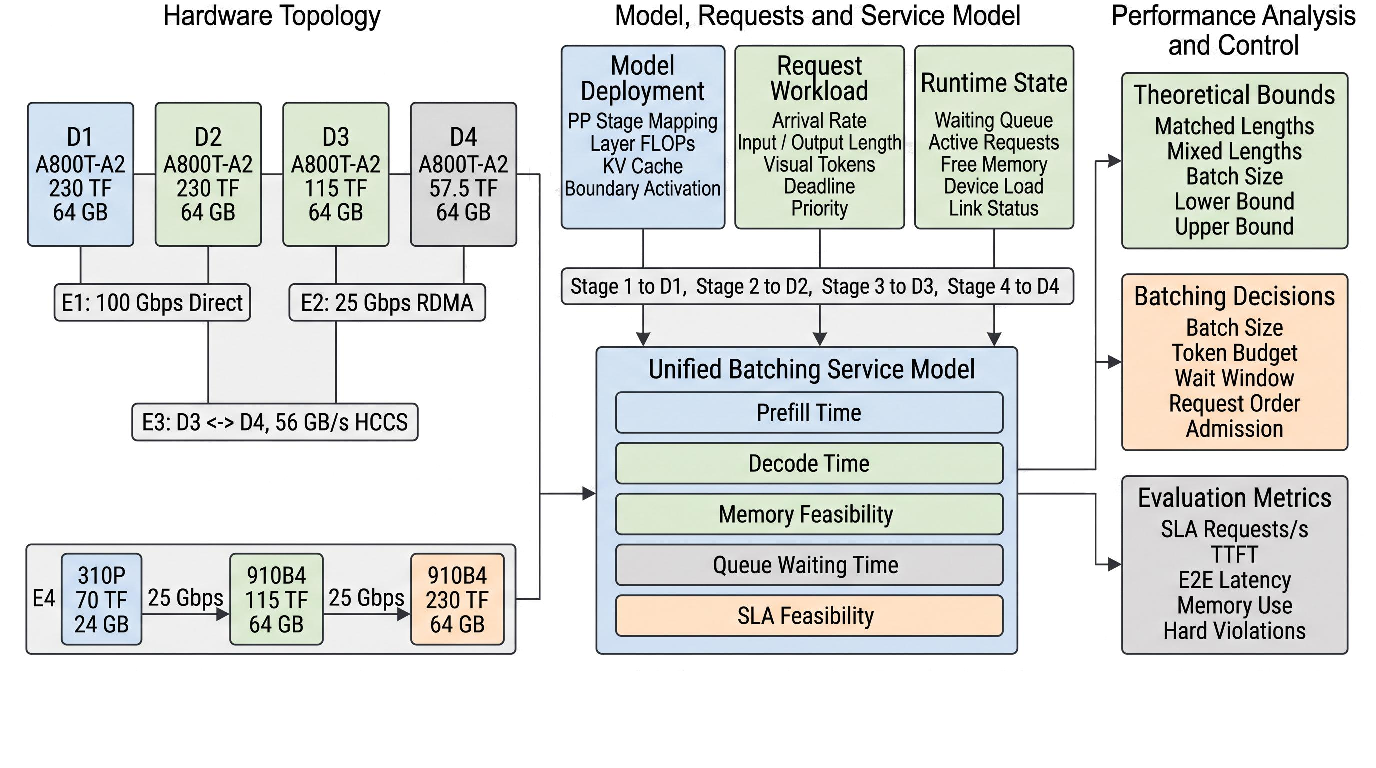
\includegraphics[width=\textwidth]{figures/ch5_system_model.pdf}
\caption{面向异构设备的业务感知 batching 系统模型}
\label{fig:ch5-system-model}
\end{figure}

硬件环境表示为图 \(\mathcal H=(\mathcal V,\mathcal E)\)。设备节点 \(g\in\mathcal V\) 记录当前可用算力 \(F_g\)、可用显存 \(M_g\) 和运行状态，链路 \((g,g')\in\mathcal E\) 记录有效带宽 \(B_{g,g'}\) 与固定传输时延 \(L_{g,g'}\)。模型沿用第四章确定的非均匀 PP 部署方案 \(\mathcal D\)，其中包含各 stage 的放置设备、连续 layer 边界以及相邻 stage 之间的 activation 传输路径。对于 stage \(k\)，其有效算力记为 \(F_k^{\mathcal D}\)，prefill 与 decode 的实测计算效率分别记为 \(\eta_{k}^{\mathrm{pre}}\) 和 \(\eta_{k}^{\mathrm{dec}}\)。

到达系统的请求 \(r_i\) 由到达时间 \(a_i\)、文本输入长度 \(P_i\)、visual token 数 \(V_i\)、预测输出长度 \(\widehat O_i\)、实际输出长度 \(O_i\)、请求 deadline \(d_i\) 和业务优先级 \(\kappa_i\) 描述。纯文本请求令 \(V_i=0\)。实际输出长度 \(O_i\) 在请求完成后用于评价预测误差和服务结果，在线决策只能读取 \(\widehat O_i\)。控制器在每个决策窗口读取等待队列、active requests、各请求的剩余时限、近期到达率、KV Cache 占用、剩余显存和设备利用率，并决定下一窗口的组批参数与请求顺序。

模型计算量直接由网络结构和请求长度得到。设一个文本 Transformer layer 的参数量为 \(N_{\mathrm{layer}}\)，hidden size 为 \(h\)。长度为 \(P\) 的单请求 prefill 计算量和生成 \(O\) 个 tokens 的 decode 计算量分别为
\[
C_{\mathrm{pre}}(P)=
\sum_{l=1}^{L}\left(2PN_l+4P^2h_l\right),
\]
\[
C_{\mathrm{dec}}(P,O)=
\sum_{u=1}^{O}\sum_{l=1}^{L}
\left(2N_l+4(P+u)h_l\right).
\]
第一式中的线性项来自模型参数参与的矩阵计算，二次项来自 prefill attention；第二式逐 token 累加 decode 计算。CodeLlama34B 使用 48 个文本 layers 的参数。Qwen2-VL-7B-Instruct 还要加入视觉编码器和模态投影的计算量，并把文本 decoder 的上下文长度写为 \(P+V\)。因此，图像数量、分辨率和预处理后 visual token 数会同时影响 prefill 时间与后续 decode 的上下文长度。

对部署 \(\mathcal D\) 中的 stage \(k\)，batch 的 prefill 服务时间由该 stage 承担模块的 FLOPs、有效算力和通信共同计算：
\[
T_{k}^{\mathrm{pre}}(b,P,V)=
\frac{C_{k}^{\mathrm{pre}}(b,P,V)}
{\eta_{k}^{\mathrm{pre}}F_k^{\mathcal D}}\times10^3
+T_{k}^{\mathrm{link,pre}}.
\]
单轮 decode 时间 \(T_{k}^{\mathrm{dec}}(b,P,V,u)\) 采用相同形式，其中计算量对应当前 token 步 \(u\)。对单个请求，完整 prefill 时间和生成 \(O\) 个 tokens 的 decode 时间分别为
\[
T_{\mathcal D}^{\mathrm{pre}}=\sum_k T_k^{\mathrm{pre}},
\qquad
T_{\mathcal D}^{\mathrm{dec}}=\sum_{u=1}^{O}\sum_k T_k^{\mathrm{dec}}(u).
\]
各量均以 FLOPs、FLOPs/s 和 ms 为单位。第四章已经选择纯 PP，因此式中的通信项只包含相邻 stages 之间的 activation 传输。部署前令计算效率系数为 1，可得到由模型规格、设备有效算力和链路共同确定的时间参照；进入 Ascend 环境后，以不同 batch size 和长度下的逐层执行时间以及 CANN/HCCL 通信时间更新效率和通信项。由此形成的 prefill/decode 服务时间曲线直接用于 SLA 仿真和 Safe-RL 训练。

显存约束同时计入模型权重、activation、KV Cache 和运行时预留。设 batch 中 active requests 的当前上下文长度为 \(\ell_i\)，单 token KV Cache 大小为 \(m_{\mathrm{KV}}\)，则 KV 占用近似为 \(m_{\mathrm{KV}}\sum_i\ell_i\)。该值与各 stage 已驻留权重和运行时空间共同决定当前能够接纳的请求数及 token budget。

\subsubsection*{5.5.2 性能理论分析}
\addcontentsline{toc}{subsubsection}{5.5.2 性能理论分析}

在统一系统模型下，本文以 Static-FIFO 为基线，先分析不同请求组合产生的长度补齐计算，再判断在线算法能够减少其中多少开销。当一个最长请求与其余最短请求进入同一 batch 时，Static-FIFO 的冗余计算最多，对应所考察请求范围内的计算侧提升上界。在此基础上，有限窗口长度感知算法给出受到观察范围和请求顺序限制时的可实现预估，进一步改变 batch size 还可以分析批内请求数量对两类结果的影响。这些结果为 Safe-RL 选择需要观察的请求特征、需要调节的 batching 参数以及合理的性能目标提供理论依据；SLA、排队、KV Cache 和控制开销的影响则在 5.5.6 节通过请求轨迹实验验证。

对于请求 \(r_i\)，将完成其 prefill 和 decode 所需的模型计算量记为
\[
C_i=C_{\mathrm{pre}}(P_i,V_i)+C_{\mathrm{dec}}(P_i,V_i,O_i).
\]
下文用 \(C(P,V,O)\) 表示具有给定输入、视觉和输出长度的请求计算量，因此 \(C_i=C(P_i,V_i,O_i)\)。
设一个静态 batch 包含 \(B\) 个请求。若执行过程按 batch 内最长输入和最长输出进行长度补齐（padding），记 \(P_{\max}\)、\(V_{\max}\) 和 \(O_{\max}\) 为该 batch 的最大长度，则总计算量近似为
\[
W_{\mathrm{pad}}=
B\,C(P_{\max},V_{\max},O_{\max}).
\]
当长度相近的请求被放在一起，并且短请求结束后空出的执行位置能够及时回收时，请求集合至少要完成的有效计算量为
\[
W_{\mathrm{use}}=\sum_{i=1}^{B}C_i.
\]
两者的比值
\[
S_{\mathrm{len}}=\frac{W_{\mathrm{pad}}}{W_{\mathrm{use}}}
\]
给出长度重排在该简化模型中的计算侧速度倍数上界。相对 Static-FIFO 的提升为 \((S_{\mathrm{len}}-1)\times100\%\)。\(S_{\mathrm{len}}\) 是无量纲的速度倍数；实际 requests/s 由服务时间模型或硬件实测得到，并进一步接受显存、排队和 deadline 检查。

表~\ref{tab:ch5-model-workload} 给出代表性请求的模型计算量和部署前服务时间。CodeLlama34B 采用 512-token 输入和 256-token 输出；Qwen2-VL-7B-Instruct 采用 640 个 visual tokens、1024 个 text tokens 和 256-token 输出。时间计算使用第四章 E1 场景中选出的 PP 部署，CodeLlama34B 的文本层分配为 \((18,18,9,3)\)，Qwen2-VL-7B-Instruct 为 \((4,14,7,3)\)。计算同时计入各 stage 的有效算力和 100~Gbps 链路上的边界 activation 传输，batch size 取 1，计算效率系数取 1。

\begin{table}[!htbp]
\centering
\small
\setlength{\tabcolsep}{5pt}
\renewcommand{\arraystretch}{1.18}
\caption{代表性请求的模型计算量与 E1 部署前服务时间}
\label{tab:ch5-model-workload}
\begin{tabularx}{\textwidth}{>{\raggedright\arraybackslash}X>{\centering\arraybackslash}m{0.15\textwidth}>{\centering\arraybackslash}m{0.15\textwidth}>{\centering\arraybackslash}m{0.17\textwidth}>{\centering\arraybackslash}m{0.17\textwidth}}
\hline
模型与请求配置 & Prefill / TFLOPs & Decode / TFLOPs & Prefill / ms & Decode / ms \\
\hline
CodeLlama34B，512 / 256 tokens & 34.43 & 17.27 & 207.84 & 104.23 \\
Qwen2-VL-7B-Instruct，640 visual + 1024 text / 256 output & 27.19 & 3.53 & 177.78 & 24.53 \\
\hline
\end{tabularx}
\end{table}

表中的时间用于把 FLOPs 计算与具体设备、链路联系起来。实际 batch size 增大后，将批内所有请求的 FLOPs 和 activation 大小代入同一公式即可得到对应服务时间。Ascend kernel 的实际利用率通常随 batch size 和序列长度变化，因此正式实验以逐层测量得到的 \(\eta_k^{\mathrm{pre}}\)、\(\eta_k^{\mathrm{dec}}\) 和通信时间替换部署前参照，再判断 TTFT、TPOT 和 E2E latency 是否满足 SLA。

对任一 batching 配置 \(a\)，将其 batch size、请求长度和执行顺序代入服务时间曲线，可以得到完成该批请求所需的时间 \(\widehat T(a)\)，并进一步估计各请求的等待时间、TTFT 和 E2E latency。记 \(\mathcal A_{\mathrm{SLA}}\) 为同时满足显存限制和 SLA 阈值的配置集合，\(B(a)\) 为配置 \(a\) 完成的请求数，则部署前的 SLA 吞吐上界写为
\[
R_{\mathrm{SLA}}^{\mathrm{ub}}=
\max_{a\in\mathcal A_{\mathrm{SLA}}}
\frac{B(a)\times10^3}{\widehat T(a)}
\quad \mathrm{requests/s}.
\]
输入长度和 visual token 数主要改变 prefill 时间，输出长度改变 decode 轮数，batch size 同时影响计算效率、KV Cache 和等待时间，因此这些参数都会改变可行配置集合与吞吐上界。正式实验使用 Ascend 实测服务时间重新计算 \(\widehat T(a)\)，并通过请求轨迹验证预测的 SLA 可行性。

理论上界用于界定请求重排的最大优化空间，可实现的部署前预估则由有限窗口长度感知组批得到。每次准备新 batch 时，调度器观察等待队列前 \(W\) 个请求，先选择剩余 TTFT 时间最短的请求作为本批的基准请求，以避免长度匹配导致紧急请求继续等待；随后利用 5.5.1 节的服务时间模型估计其余请求的 prefill 和 decode 执行开销，从中选择预计执行开销最接近的 \(B-1\) 个请求。请求加入后还要单独检查 KV Cache、显存和 SLA，检查失败时跳过该请求并继续考察下一个。部署前分析以 \(B=8\) 为参考 batch size，并令观察范围为其三倍，即 \(W=24\)；后续再改变 \(W\) 和 \(B\) 检查结果的敏感性。

为了在相同计算口径下比较理论空间与有限窗口算法，记 Static-FIFO 形成的所有 batches 的长度补齐计算量为 \(W_{\mathrm{FIFO}}\)，全部请求自身所需的有效计算量为 \(W_{\mathrm{use}}\)，有限窗口长度感知算法形成的 batches 的长度补齐计算量为 \(W_{\mathrm{len}}\)。处理相同数量请求时，两种提升分别为
\[
G_{\mathrm{ub}}=\frac{W_{\mathrm{FIFO}}}{W_{\mathrm{use}}}-1,
\qquad
G_{\mathrm{len}}=\frac{W_{\mathrm{FIFO}}}{W_{\mathrm{len}}}-1.
\]
其中，\(G_{\mathrm{ub}}\) 表示完全消除额外长度补齐计算时的上界，\(G_{\mathrm{len}}\) 表示在 \(W=24\)、\(B=8\) 条件下执行上述排序算法得到的预估提升。两者均使用 5.5.1 节的模型 FLOPs 计算，不再使用输入输出 token 数的线性加权值。

表~\ref{tab:ch5-length-aware-estimate} 使用短、中、长三档请求进行计算。CodeLlama34B 的输入长度为 128、512 和 2048 tokens，Qwen2-VL-7B-Instruct 的文本输入长度为 256、1024 和 4096 tokens，并固定 640 个 visual tokens；输出长度均为 64、256 和 512 tokens。计算侧预估令同一观察窗口中的请求均已到达且 SLA 紧迫程度相同，因而只比较长度补齐计算量；请求到达和 deadline 的影响在随后请求轨迹中加入。

\begin{table}[!htbp]
\centering
\small
\setlength{\tabcolsep}{4pt}
\renewcommand{\arraystretch}{1.18}
\caption{短、中、长三档随机请求下的纯计算上界与有限窗口排序预估}
\label{tab:ch5-length-aware-estimate}
\begin{tabularx}{\textwidth}{>{\raggedright\arraybackslash}X>{\centering\arraybackslash}m{0.16\textwidth}>{\centering\arraybackslash}m{0.16\textwidth}>{\centering\arraybackslash}m{0.16\textwidth}>{\centering\arraybackslash}m{0.16\textwidth}}
\hline
请求分布 & \multicolumn{2}{c}{CodeLlama34B} & \multicolumn{2}{c}{Qwen2-VL-7B-Instruct} \\
 & 计算上界 & 排序预估 & 计算上界 & 排序预估 \\
\hline
输入输出长度一致 & 0.0\% & 0.0\% & 0.0\% & 0.0\% \\
仅输入长度变化 & 135.5\% & 115.3\% & 103.1\% & 89.5\% \\
仅输出长度变化 & 35.7\% & 32.8\% & 11.8\% & 11.0\% \\
输入输出长度同时变化 & 173.3\% & 111.9\% & 115.7\% & 90.1\% \\
\hline
\end{tabularx}
\end{table}

输入长度变化带来的提升高于输出长度变化，主要原因是较长 prompt 会同时增加参数计算和 attention 计算，并把静态 batch 中其它短请求的 prefill 长度一并抬高。表中的有限窗口排序只能观察队首 24 个请求，因此预估结果低于可以在全部请求中自由匹配的计算上界；加入真实到达时间和 deadline 后，紧急请求优先还会进一步限制长度匹配空间。在输入输出长度同时变化时，CodeLlama34B 的纯计算上界为 173.3\%，有限窗口排序预估为 111.9\%；Qwen2-VL-7B-Instruct 的两项结果分别为 115.7\% 和 90.1\%。这些数值用于描述组批算法自身能够减少多少长度补齐计算，尚未计入请求等待、显存限制和 SLA 筛选。

将上述规则应用于带到达时间、输入输出长度和 deadline 的请求轨迹后，可以得到实际形成的 batch 序列。每个 batch 的完成时间由 \(\widehat T(a)\) 计算，请求等待时间由到达时刻与 batch 启动时刻之差得到。设轨迹持续时间为 \(T_{\mathrm{trace}}\)，单位为 s，其中满足 SLA 并完成的请求数为 \(N_{\mathrm{SLA}}\)，则该规则的预估请求处理速度为
\[
\widehat R_{\mathrm{len}}=
\frac{N_{\mathrm{SLA}}}{T_{\mathrm{trace}}}
\quad \mathrm{requests/s}.
\]
在相同请求轨迹上运行 Static-FIFO，即可由 \(\widehat R_{\mathrm{len}}/\widehat R_{\mathrm{FIFO}}-1\) 得到长度感知组批的预估提升。该结果反映有限观察范围、请求到达顺序和 SLA 共同约束下能够实现的参考性能，并作为 Safe-RL 设计与实验结果之间的中间参照。

为了观察极端长度失配对计算上界的影响，进一步使用 \(B=64\) 的请求集合进行比较。CodeLlama34B 的输入长度取 128、512 和 2048 tokens，Qwen2-VL-7B-Instruct 取 256、1024 和 4096 text tokens，并固定 640 个 visual tokens；输出长度取 64、256 和 512 tokens。对 decode 而言，长度匹配最好的情况是 64 个请求具有相同的输出 token 数；同时计入 prefill 后，还要求输入长度一致，此时没有额外的长度补齐计算。输出失配场景由 1 个 512-token 输出和 63 个 64-token 输出组成，输入失配场景由 1 个最长输入和 63 个最短输入组成。本文将“1 个最长输入、最长输出请求与 63 个最短输入、最短输出请求”定义为组合失配的最差情况。表~\ref{tab:ch5-batching-extreme-bound} 给出这些极端组合下的纯计算上界。

\begin{table}[!htbp]
\centering
\small
\setlength{\tabcolsep}{4pt}
\renewcommand{\arraystretch}{1.18}
\caption{64 个请求极端长度组合下的纯计算上界}
\label{tab:ch5-batching-extreme-bound}
\begin{tabularx}{\textwidth}{>{\raggedright\arraybackslash}X>{\centering\arraybackslash}m{0.20\textwidth}>{\centering\arraybackslash}m{0.20\textwidth}>{\raggedright\arraybackslash}X}
\hline
请求组成 & CodeLlama34B 上界 & Qwen2-VL 上界 & 含义 \\
\hline
输入输出长度完全一致 & 0.0\% & 0.0\% & 静态组批已无长度补齐损失 \\
仅输出长度极端失配 & 76.1\% & 21.7\% & 长输出持续占用 batch 执行周期 \\
仅输入长度极端失配 & 478.6\% & 280.8\% & 最长 prompt 放大整个 batch 的 prefill 计算 \\
输入输出同时极端失配 & 1060.2\% & 353.9\% & 长输入与长输出的影响叠加 \\
\hline
\end{tabularx}
\end{table}

输入长度带来的范围明显大于输出长度，主要原因是 prefill attention 中包含随输入长度平方增长的计算项。Qwen2-VL 的视觉编码开销对每个请求都存在，因而长度失配占总计算量的比例低于 CodeLlama34B。组合失配中的大幅提升描述 1 个最长请求与 63 个最短请求被强制放入同一静态 batch 的极端情况，用于界定算法层面的最大空间；在线策略还要服从到达顺序、deadline、显存和等待时间限制。

batch size 越大，一个极长请求影响的其它请求越多。表~\ref{tab:ch5-batchsize-bound} 固定组合失配模式，比较不同 \(B\) 下的理论上界。

\begin{table}[!htbp]
\centering
\small
\setlength{\tabcolsep}{7pt}
\renewcommand{\arraystretch}{1.18}
\caption{batch size 对组合失配理论上界的影响}
\label{tab:ch5-batchsize-bound}
\begin{tabular}{c c c}
\hline
Batch size / requests & CodeLlama34B 提升 & Qwen2-VL 提升 \\
\hline
8  & 432.7\% & 225.8\% \\
16 & 671.0\% & 288.4\% \\
32 & 893.1\% & 329.7\% \\
64 & 1060.2\% & 353.9\% \\
\hline
\end{tabular}
\end{table}

较大的 batch 为长度重排提供更多空间，也会增加 KV Cache、单轮执行时间和 TTFT 风险。表中的上界用于界定长度重排的优化空间，Safe-RL 的实际收益还受到可观察请求数、SLA 允许的等待时间、显存和运行时开销影响。算法在这些条件下联合调整 batch 容量、token budget 与请求顺序。进入硬件环境后，再使用 Ascend 实测的 prefill 和 decode 服务时间校准理论结果。

\subsubsection*{5.5.3 基于安全强化学习的 Batching 算法}
\addcontentsline{toc}{subsubsection}{5.5.3 基于安全强化学习的 Batching 算法}

前述理论分析表明，请求长度、batch size 和可观察请求范围都会改变 batching 的优化空间；在线系统还要同时处理到达率、KV Cache、deadline、prefill/decode 干扰和运行时能力。若为这些变量逐项设置阈值，规则数量会快速增加，并且一次调整对后续队列和显存的影响难以由局部规则评价。强化学习能够从连续运行反馈中学习多变量之间的关系，因此适合用于动态 batching 控制。

现有系统已经提供了必要的执行基础。Orca \cite{yu2022orca} 支持迭代级调度，vLLM \cite{kwon2023efficient} 提供灵活的 KV Cache 管理，Sarathi-Serve \cite{agrawal2024taming} 和 DistServe \cite{zhong2024distserve} 分别利用 chunked prefill 与 prefill/decode 分离缓解阶段干扰，JITServe \cite{zhang2026jitserve} 和 SOLA \cite{hong2025sola} 进一步考虑 deadline。这些机制扩大了可调节的参数和执行方式，也使固定规则更难覆盖全部组合。

普通强化学习策略在训练探索、负载突变和状态估计误差下可能输出越界动作。本文采用 Safe-RL 将长期风险约束与当前窗口的确定性安全检查结合起来。Actor 根据请求、资源和 SLA 状态提出 batching 方案，Critic（价值评估网络）根据后续运行结果评价该方案的长期完成请求数与风险；拉格朗日约束用于限制多个窗口上的累计风险，安全投影在动作下发前检查显存、deadline 和运行时支持范围。无法修正的动作回退到最近的稳定配置。

图~\ref{fig:ch5-batching-architecture} 给出了完整闭环。系统先采集队列、请求长度、KV Cache 和 SLA 状态，Actor 输出 batch 参数、请求排序和执行机制，安全投影生成可执行配置，推理运行时返回完成请求数、时延、资源占用和违规事件，反馈再用于更新 Actor、Critic 和约束模型。该方法的重点是在动态提高完成请求速度的同时，使受控压力实验中的 OOM、不可执行动作和已接纳关键请求硬超时均保持为 0。

\begin{figure}[!htbp]
\centering
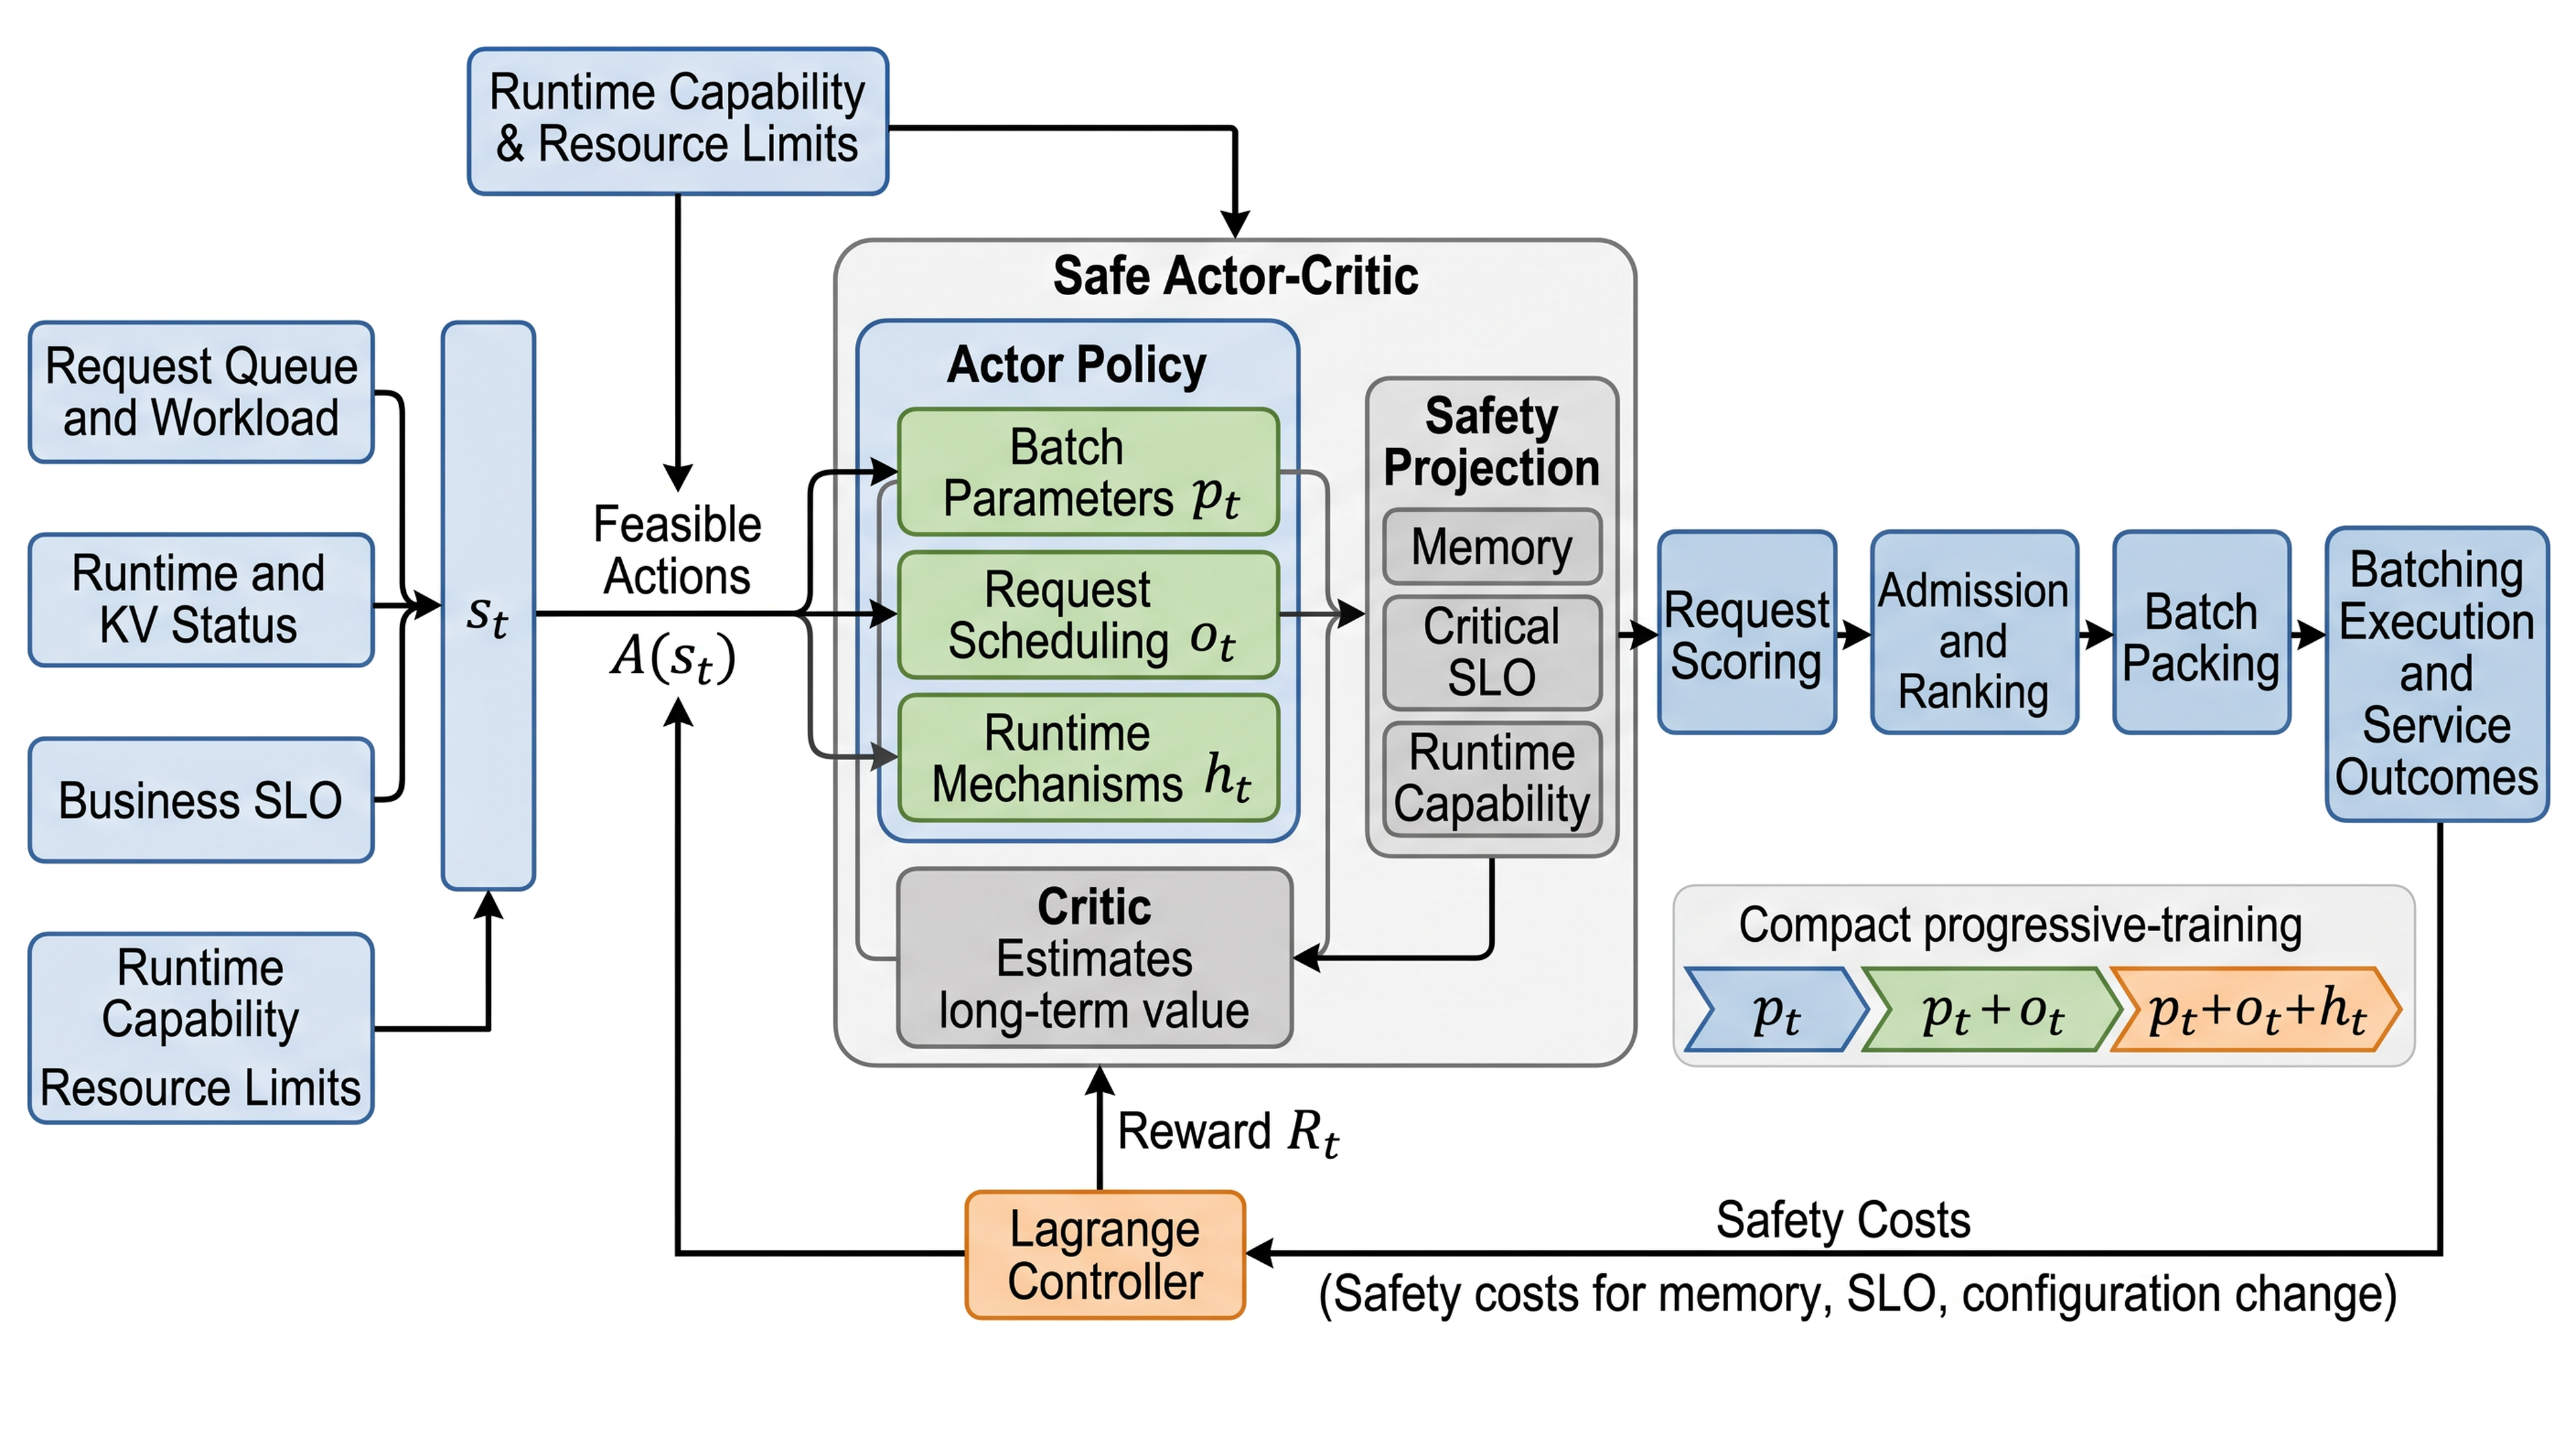
\includegraphics[width=0.88\textwidth]{figures/ch5_safe_rl_batching.png}
\caption{基于拉格朗日约束和安全投影的在线 batching 优化架构}
\label{fig:ch5-batching-architecture}
\end{figure}

\subsubsection*{5.5.4 CMDP 建模与决策生成}
\addcontentsline{toc}{subsubsection}{5.5.4 CMDP 建模与决策生成}

连续 batching 控制可以写成约束马尔可夫决策过程（Constrained Markov Decision Process，CMDP）。这一模型描述一次配置调整对后续队列、KV Cache 和请求时限的持续影响，并进一步规定 Actor 的输出如何转换为实际 batch，使各项决策都有明确的数据来源和运行时取值范围。

本文将推理过程划分为控制窗口 \(t=0,1,\ldots\)，每个窗口依次完成状态采集、动作生成、运行执行和反馈更新。CMDP 表示为
\[
\mathcal M=(\mathcal S,\mathcal A,\mathcal P,R,\{\xi^j\},\gamma),
\]
其中，\(\mathcal S\) 和 \(\mathcal A\) 分别为状态空间与动作空间，\(\mathcal P\) 描述执行动作后的状态变化，\(R\) 表示服务收益，\(\xi^j\) 表示第 \(j\) 类运行风险，\(\gamma\) 用于降低较远反馈对当前决策的影响。

窗口开始时的状态记为 \(s_t=(q_t,z_t,d_t)\)。\(q_t\) 包含等待队列、active requests、prefill/decode 请求数、近期到达率和输入输出长度分布；\(z_t\) 包含可用显存、剩余 KV blocks、设备利用率、近期服务时间、链路状态、上一窗口配置和运行时支持能力；\(d_t\) 包含请求优先级、deadline 及其剩余时间。模型结构、单 token KV Cache 大小和 5.5.1 节得到的 prefill/decode 服务时间曲线作为相对稳定的上下文输入。

动作 \(a_t\) 包含三类决策。第一类是 batch 容量参数，包括 active batch 上限 \(b_t\)、token budget \(u_t\)、最大等待窗口 \(w_t\)、prefill chunk size \(c_t\) 和 prefill/decode 配额 \(\rho_t\)。第二类是请求调度参数，包括准入阈值 \(\tau_t\) 与请求排序权重 \(\vec{\omega}_t\)。第三类是运行时机制 \(h_t\)，用于选择当前环境已经支持的 chunked prefill、长请求隔离或 PD 资源池路由。容量参数和调度参数在短周期更新，切换开销较高的机制在较长周期更新。

这些决策变量由运行状态逐步生成。系统先读取 Ascend 推理运行时支持的参数、取值范围和调整粒度；再依据实例并发上限、剩余 KV blocks 和单 token KV 增量确定 \(b_t\) 与 \(u_t\) 的上界，依据 deadline、队列积压和到达率限制 \(w_t\) 与 \(\tau_t\)，并依据 token 粒度和当前 prefill/decode 积压确定 \(c_t\) 与 \(\rho_t\) 的可选范围。Actor 输出归一化数值后，将其映射到这些范围并按运行时粒度取整。对于离散机制，当前环境不支持的选项在 Actor 输出阶段直接屏蔽。

请求排序权重进一步转换为 batch 成员。等待请求 \(r_i\) 的得分为
\[
S_i=\omega_1 f_{\mathrm{urgency}}(r_i)
+\omega_2 f_{\mathrm{age}}(r_i)
+\omega_3 f_{\mathrm{priority}}(r_i)
-\omega_4 f_{\mathrm{cost}}(r_i)
-\omega_5 f_{\mathrm{KV}}(r_i).
\]
距离 deadline 越近、等待越久或业务优先级越高，请求得分越高；预计 FLOPs、输出长度和 KV 增量越大，其资源成本越高。系统按得分选择满足准入阈值的请求，并同时检查请求数不超过 \(b_t\)、总 token 数不超过 \(u_t\)。等待时间项持续增长，使长请求和低优先级请求仍能获得执行机会。

窗口收益以完成请求数为主要正向项，并扣除归一化的排队时间和 E2E latency，使策略同时学习提高处理速度和缩短响应时间。风险包括 OOM 与不可执行配置、TTFT/TPOT/E2E 超限、长请求等待过久和相邻窗口配置变化过大。策略在这些风险上限内提高长期服务收益：
\[
\max_{\pi} J_R(\pi),
\qquad
J_j(\pi)\leq\epsilon_j.
\]
其中，\(J_R\) 是多个控制窗口上的累计服务收益，\(J_j\) 是第 \(j\) 类累计风险，\(\epsilon_j\) 是相应上限。硬系统事件和已接纳关键请求硬超时的上限取 0，分位 SLA、公平性和配置变化采用业务允许值。完成请求数、等待时间和 E2E latency 的权重在训练集上固定，并在全部对比实验中保持一致。Actor 输出的建议动作还要经过下一节的安全投影后才能下发。

\subsubsection*{5.5.5 策略学习与安全执行}
\addcontentsline{toc}{subsubsection}{5.5.5 策略学习与安全执行}

Safe-RL 需要同时处理跨窗口的性能收益和当前窗口的执行安全。Actor 负责提出联合 batching 方案，Critic（价值评估网络）根据后续队列、显存和请求时延变化评价该方案。拉格朗日约束影响训练方向，安全投影负责动作下发前的最终检查，两者共同覆盖长期风险和单次执行安全。

Actor 策略记为 \(\pi_{\theta}(a_t\mid s_t)\)。训练时引入非负风险系数 \(\mu_j\)，将窗口收益调整为
\[
\widetilde R_t=R_t-\sum_j\mu_j\xi_t^j.
\]
当某类风险接近上限时，对应系数增大，Critic 会降低高风险动作的长期评价；风险保持较低时，策略可以继续探索提高完成请求数的配置。Critic 依据实际执行后的状态与收益更新价值估计，Actor 再提高长期评价较好动作的选择概率。部署阶段使用策略均值或最高概率动作，减少随机输出造成的配置波动。

拉格朗日约束根据历史轨迹控制多个窗口上的累计风险，实际系统还需要在每次动作下发前进行确定性检查。将 Actor 提出的动作记为 \(\widetilde a_t\)，经过检查后实际下发的动作记为 \(\widehat a_t\)，二者满足
\[
\widehat a_t=\Pi_{\mathcal A_{\mathrm{safe}}(s_t)}(\widetilde a_t),
\]
其中，\(\Pi\) 表示把建议动作修正到安全范围内的确定性映射，\(\mathcal A_{\mathrm{safe}}(s_t)\) 是当前状态下同时满足显存、已接纳关键请求 deadline 和推理运行时能力要求的动作集合。轻量性能模型先预测建议动作对应的峰值显存、关键请求 TTFT、decode ITL 和单轮执行时间，再加入根据离线预测误差设置的安全余量。修正后的预测结果通过全部约束检查后，动作才会进入推理运行时。显存容量和运行时支持项可以直接检查，时延条件则依据带安全余量的预测上界判断；安全压力实验进一步统计实际执行中的 OOM、硬超时和不可执行动作，用于确认零硬违规目标。

具体来说，若预测显存超限，投影模块先缩小 token budget 或 active batch 上限，并重新选择 batch 成员；若已接纳的关键请求可能错过 deadline，则缩短等待窗口、提高紧迫度权重，并把执行配额转向该请求当前所处的 prefill 或 decode 阶段，同时减少与其无关的工作；当前推理运行时不支持的机制则直接关闭。连续参数被调整到最近的可执行值，离散机制只能从支持列表中选择。若多次修正后仍找不到可行动作，系统回退到上一稳定配置，并优先处理已经接纳的关键请求。只有当负载超过物理承载能力时，才在准入阶段对新请求限流，并将限流结果单独统计。

训练轨迹同时记录建议动作 \(\widetilde a_t\)、实际动作 \(\widehat a_t\)、修改幅度和运行结果。Critic 根据实际执行后的状态变化进行评价；如果 Actor 频繁提出需要大幅修正的动作，训练信号会加入额外惩罚。随着训练进行，策略应逐步减少对投影和回退的依赖，直接生成更接近安全范围的配置。

运行时采集请求长度、TTFT、ITL、E2E latency、KV Cache 使用量、违规和回退信息，并反馈给 Actor、Critic 与约束模块，形成图~\ref{fig:ch5-batching-architecture} 所示的闭环。短周期负责更新 batch 参数和请求调度，长周期负责切换开销较高的执行机制。拉格朗日约束用于降低多个窗口上的累计风险，安全投影用于拦截当前窗口中预测会越界的动作，两个控制周期则避免高开销机制频繁切换。

为降低在线探索风险，训练分三步进行：首先固定 FIFO 和运行时机制，只训练 batch 容量参数；随后加入请求准入与排序；最后联合优化 batch 参数、请求调度与执行机制。

这种顺序逐步扩大动作空间，使 Critic 能够区分容量调整、请求排序和机制切换的影响，并减少训练初期配置反复变化的情况。

训练初期使用静态 batching、FIFO 和启发式策略生成离线训练数据。在线阶段先只计算建议配置并评估其可行性，不实际下发；确认性能模型误差可控后，再允许策略在安全范围内尝试小幅调整，并保留稳定配置作为回退。性能模型通过离线性能测量和在线数据持续更新。在线控制器以静态 batching 和固定请求顺序作为参照，并以前文给出的性能与安全目标作为训练和验证依据；具体收益在下一节结合基础仿真和正式实验进行分析。

\subsubsection*{5.5.6 实验设计与评价指标}
\addcontentsline{toc}{subsubsection}{5.5.6 实验设计与评价指标}

Safe-RL 的验证由服务时间标定、请求轨迹回放和安全压力测试组成。实验先用 5.5.1 节的 FLOP 模型确定需要测量的输入长度、输出长度和 batch size 组合，再以 Ascend 上的实测 prefill/decode 时间替代理论计算中的效率系数。所有策略使用相同模型部署、请求到达时间、请求属性和随机种子，并按照“先满足 SLA 与硬安全要求，再比较完成请求速率和平均 E2E latency”的顺序评价。

性能标定覆盖 CodeLlama34B 和 Qwen2-VL-7B-Instruct，并沿用第四章最终选择的模型部署。对每个模型分别改变输入长度、输出长度、visual token 数、active batch、token budget、KV Cache 占用和 prefill/decode 配额，测量各 stage 的 prefill 时间、单轮 decode 时间、通信时间和峰值显存。这些数据形成 \(T^{\mathrm{pre}}_{\mathcal D}\) 与 \(T^{\mathrm{dec}}_{\mathcal D}\) 服务时间曲线，用于离线训练、SLA 仿真和安全投影。

主负载采用 4 到配置上限之间随机变化的闭环并发。每隔 500~ms 更新目标并发；并发升高时增加客户端，并发降低时等待已有请求完成后停止补充。请求输入和输出均覆盖短、中、长三档，Qwen2-VL-7B-Instruct 额外改变图像数量、分辨率和 visual token 数。业务优先级按高、普通和低三档混合，并为高优先级请求设置更严格的 deadline。正式测试覆盖给定的 11 组模型、组网、P90/P99 TTFT 和并发配置 \cite{huawei2026internal}，各方法使用相同的到达轨迹、请求属性和随机种子。

设统计窗口长度为 \(T\) s，窗口内提交并最终完成的请求数为 \(N_T^{\mathrm{done}}\)，则完成请求速率为
\[
\widehat R_{\mathrm{thr}}=
\frac{N_T^{\mathrm{done}}}{T}.
\]
平均 E2E latency 为
\[
\overline L_{\mathrm{E2E}}=
\frac{1}{N_T^{\mathrm{done}}}
\sum_{i\in\mathcal R_T}(f_i-a_i).
\]
其中，\(\widehat R_{\mathrm{thr}}\) 的单位为 requests/s；\(\mathcal R_T\) 是统计窗口内提交并最终完成的请求集合，\(a_i\) 和 \(f_i\) 分别为请求到达与完成时间，单位为 ms。窗口结束后停止提交新请求并排空队列，使平均时延覆盖窗口内提交的全部请求。未通过 SLA 或安全检查的运行点保留失败原因和时延记录，其完成请求速率不参与可行策略之间的性能比较。

主对比包括两类基线和三种 RL 方法。基线为 Static-FIFO、Ascend 推理运行时默认配置和 SLA-Heuristic；RL 方法为 Unconstrained-RL、Lagrangian-RL 和完整 Safe-RL。Static-FIFO 使用固定 batch size、等待窗口和 token budget，按到达顺序形成批次，并在当前批次完成后再处理下一批；SLA-Heuristic 按 deadline 和长度设置人工规则；Unconstrained-RL 只优化性能；Lagrangian-RL 加入长期风险约束；Safe-RL 进一步加入当前窗口的安全投影和回退。六种方法使用相同的硬件资源、请求范围和运行时能力。

实验分别改变输入长度分布、输出长度分布、batch size、可观察请求数、最大等待时间、token budget、prefill chunk size、prefill/decode 配额、输出长度预测误差、并发变化速度和 SLA 严格程度。低并发场景用于观察调度空间不足时的控制开销，中高并发和长度混合场景用于检验算法能否利用 5.5.2 节给出的理论空间。固定并发扫描用于确定各方法满足 SLA 的最大稳定并发，随机并发轨迹用于比较动态负载下的完成请求速率和平均 E2E latency。

实验需要验证三项结论：Safe-RL 能否在满足 SLA 的前提下提高完成请求速率并降低平均 E2E latency；拉格朗日约束和安全投影能否实现零硬违规；batch 容量、请求排序和运行时机制分别贡献多少收益。除随机并发主实验外，还设置稳定负载、阶跃负载、短时突发、长 prompt 集中到达、不同 prefix cache 命中率以及 prefill-heavy、decode-heavy 场景。训练与测试使用不同的请求序列和随机种子。

第一组实验回放上述随机并发轨迹。每种策略使用相同的请求到达时间、输入输出长度、优先级和随机种子。校准阶段在相同的 batch size、观察范围、最大等待时间、token budget、prefill chunk size 和 prefill/decode 配额范围内调节方法：Static-FIFO 与启发式方法在训练轨迹上选择满足 SLA 的最佳固定配置，Safe-RL、Lagrangian-RL 和 Unconstrained-RL 则把同一范围作为动作边界进行训练；测试阶段固定各方法在训练阶段得到的参数或策略。每个测试运行点先检查 P90/P99 TTFT、TPOT/E2E latency、显存使用、队列稳定性和硬安全事件；未通过检查的配置记录失败原因，通过检查的配置再比较完成请求速率、平均 E2E latency、P95/P99 latency、最长等待时间、ITL 和设备利用率。

设 Static-FIFO 和 Safe-RL 在同一条请求轨迹上均满足 SLA，其完成请求速率和平均 E2E latency 分别为 \(R_0,L_0\) 和 \(R_{\mathrm{safe}},L_{\mathrm{safe}}\)。其中，\(R_0\) 与 \(R_{\mathrm{safe}}\) 的单位为 requests/s，\(L_0\) 与 \(L_{\mathrm{safe}}\) 的单位为 ms，相应的性能目标为
\[
R_{\mathrm{safe}}\geq1.2R_0,
\qquad
L_{\mathrm{safe}}\leq0.8L_0.
\]
两个目标分别表示完成请求速率至少提高 20\% 和平均 E2E latency 至少下降 20\%，均依据同一配置、同一并发轨迹下的实测值计算。测试窗口结束后停止提交新请求并排空已有队列，平均 E2E latency 对窗口内提交的全部请求计算；同时报告到达量、完成量、拒绝量和窗口结束时的积压量。除混合请求负载的整体结果外，还分别改变输入长度分布、输出长度分布、并发水平和 SLA 严格程度，报告不同长度请求的完成请求速率、时延和最大等待时间，以检查长请求饥饿和短请求阻塞。主动限流和拒绝只在超过系统承载能力的安全压力测试中启用，并与性能主实验分开统计。

随机并发实验用于计算满足 SLA 时的完成请求速率和平均 E2E latency 改善；固定并发扫描用于补充确定各方法的最大稳定并发。与第四章方法联合使用时，以第四章理论比较最终选定的部署方案运行 Static-FIFO 所得到的实测结果作为本章基线，再计算 batching 带来的增量收益。

第二组实验验证业务感知调度。固定请求量和长度分布，改变高优先级请求比例与 deadline 紧迫程度，分别统计各优先级的 SLA 违规率、等待时间和完成率，并报告最大等待时间和 Jain 公平性指数。

第三组实验为安全压力测试。实验延长最高并发的持续时间、集中注入长 prompt，并通过预占显存或减少可用 KV block 模拟资源突然收缩。比较 Safe-RL、Lagrangian-RL 和 Unconstrained-RL 的峰值显存、OOM、不可执行动作、已接纳关键请求硬 SLA 违规、建议动作被修改的次数、回退和限流情况。零硬违规直接按三类事件的总数定义：
\[
N_{\mathrm{hard}}=
N_{\mathrm{OOM}}+N_{\mathrm{invalid}}+N_{\mathrm{deadline}}=0.
\]
其中，\(N_{\mathrm{deadline}}\) 只统计系统已经接纳的关键请求。Safe-RL 需要在所有受控压力场景中保持 \(N_{\mathrm{hard}}=0\)。同时记录 Actor 建议被安全模块修改的比例和参数修改幅度；若这些数值随训练下降，说明 Actor 正在逐步学会直接生成更接近安全范围的配置。超过系统物理处理能力的新请求单独统计限流和接纳结果。

第四组实验进行消融：依次比较仅调整 batch 容量参数、进一步加入请求排序、以及同时加入运行时机制选择的结果。对于 chunked prefill、长请求隔离和 PD 路由，额外记录启用次数、持续时间和切换开销。

每个实验点预热后至少完成 1000 个请求，并使用不少于五个随机种子重复。时延报告平均值、P95 和 P99，完成请求速率报告均值和 95\% 置信区间，同时测量状态采集、Actor 推理、安全投影和 batch 重组的控制开销。达到本节目标需要同时满足：Static-FIFO 与 Safe-RL 在相同硬件、请求轨迹和 SLA 检查下运行，Safe-RL 的完成请求速率提高不少于 20\%，统计窗口内提交请求的平均 E2E latency 下降不少于 20\%，且 \(N_{\mathrm{hard}}=0\)。
\phantomsection
\subsection*{5.6 小结}
\addcontentsline{toc}{subsection}{5.6 小结}

本章按 batch 形成和更新粒度，将业务感知 batching 参数优化划分为四类：Queue-level Dynamic / Admission Batching、Continuous Batching / Iteration-level Batching、Chunked Prefill / Blended Batching 和 Disaggregated Prefill-Decode Batching。Queue-level 方法决定请求进入执行前如何等待、排序和接纳；Continuous Batching 将 batch 更新边界推进到 decode iteration；Chunked Prefill / Blended Batching 通过切分长 prompt 并与 decode 混合执行来控制阶段干扰；Disaggregated Prefill-Decode Batching 则把 prefill 和 decode 放入不同实例或资源池中分别组批。

这四类方法对应不同的 batching 控制层次，可以在同一 runtime 中组合使用。本章将 SLO-aware、KV-aware、multi-tenant 和 speculative verification 作为横向约束或附加机制：SLO 影响 admission 和排序，KV 状态影响 active batch 容量和迁移成本，多租户影响队列公平性，speculative verification 则引入额外的验证 batch。以 batch 更新粒度为主线，可以清楚地区分“请求进不进 batch”“active set 何时更新”“prefill 是否切块混合”“两阶段是否分池组批”这几类核心问题。

CEC 场景改变了 batching 的优化重心。云端 serving 通常依赖大请求池和高速互联来扩大 batch，而单个请求入口附近的实例往往请求池较小、链路波动更强、SLO 更紧、KV 显存更有限。因此，靠近入口的实例更适合短等待窗口、低延迟 continuous batching 和保守的 chunked prefill，能够聚合多个入口或具备更强算力的协作节点则适合处理 prefill-heavy 请求、长上下文和较大的 batch。业务感知 batching 需要同时读取请求长度、SLO、优先级、KV 占用、实例负载和链路状态，并据此联合调节多个控制量。

面向验证环境，本章先用设备拓扑、第四章选定的模型部署、模型 FLOPs 和请求属性建立系统模型，由此计算不同 batch size 与输入输出长度下的 prefill/decode 服务时间。理论分析比较静态长度补齐与每个请求有效计算量，给出长度完全一致、输入失配、输出失配和组合失配下的性能范围。该分析解释了动态组批可以利用的空间，也为后续 Safe-RL 结果提供与模型和硬件条件一致的参照。

在线控制被建模为 CMDP，并采用带拉格朗日约束的 Actor-Critic 求解。Actor 联合生成 batch 容量、请求排序和运行时机制，Critic（价值评估网络）评价多个窗口上的完成请求数、响应时间与风险；安全投影在动作下发前检查显存、deadline 和运行时支持范围，无法修正时回退到稳定配置。正式实验使用 Ascend 实测服务时间曲线替代理论计算中的效率系数，并在相同 SLA 下比较 Static-FIFO、规则方法、普通 RL、Lagrangian-RL 与 Safe-RL 的完成请求速率、平均 E2E latency 和硬违规事件。

\input{sections/06-task-offloading-highlight}
\phantomsection
\section*{七、三类算法的协同优化框架}
\addcontentsline{toc}{section}{七、三类算法的协同优化框架}

前文分别从模型切分部署、业务感知 batching 和 LLM inference task offloading 三个角度讨论了 CEC-LLM 推理系统的关键算法。真实系统中，这三类算法并不是彼此独立的模块：模型切分部署决定模型组件、服务实例和推理阶段的空间分布；业务感知 batching 决定请求、prefill chunk 和 decode token 在实例内部或不同阶段资源池中的时间组织；task offloading 决定完整请求、复杂 workflow 以及 context/KV/runtime state 在端、边、云之间的路由、迁移和复用。三者共享模型位置、队列长度、KV cache 位置、链路状态、用户移动趋势和 SLO slack 等同一组系统状态，因此任何一类算法的局部优化都可能改变另外两类算法的可行域和收益。

本章不再重新划分第四、五、六章的所有单点方法，而是围绕“三类算法之间怎样协同”组织已有工作。具体而言，协同优化关注的不是某个模型如何单独切分、某个 batch size 如何单独选择，或某个请求如何单独卸载，而是这些决策在多时间尺度、多资源层级和多运行时状态下如何形成闭环。已有工作已经从局部角度揭示了这种耦合关系：model caching 会影响 request offloading 的可选路径，prefill/decode disaggregation 会改变 batching 和 KV handoff，KVCache-centric serving 会把状态位置纳入 request scheduling，移动场景下的 context migration 又会反过来影响长期 session routing。

本文将 CEC-LLM 推理中的三类算法协同关系划分为四类：
\begin{enumerate}
\item \textbf{Model / Service Placement -- Request Offloading 协同}：低频模型缓存、服务部署和高频请求路由之间的双时间尺度闭环。
\item \textbf{Model Partitioning -- Batching / Scheduling 协同}：模型切分、阶段解耦、continuous batching 和 serving scheduling 之间的容量匹配与时延控制。
\item \textbf{Request / Workflow Routing -- Runtime State Management 协同}：请求路径、agent workflow、KV cache、prefix cache、session state 和 context migration 之间的状态感知路由。
\item \textbf{Mobility-aware Hierarchical Control}：用户移动、负载热点变化、handover 和状态位置变化共同驱动的跨层闭环控制。
\end{enumerate}

这四类关系不是新的孤立算法类别，而是前文三类算法在系统运行时的交叉界面。第一类主要连接第四章的模型/服务部署和第六章的请求卸载；第二类连接第四章的模型切分和第五章的 batching；第三类连接第五章的状态感知调度和第六章的请求/workflow offloading；第四类则把移动 CEC 中的外部扰动纳入统一控制框架。表~\ref{tab:cec-collaborative-optimization-overview} 汇总了与这些协同关系直接相关的代表工作、主归属和方法关键词。

\begingroup
\scriptsize
\setlength{\tabcolsep}{1.4pt}
\renewcommand{\arraystretch}{1.35}
\emergencystretch=2em
\begin{longtable}{@{}>{\raggedright\arraybackslash\hspace{0pt}}p{0.035\textwidth} >{\raggedright\arraybackslash\hspace{0pt}}p{0.175\textwidth} >{\raggedright\arraybackslash\hspace{0pt}}p{0.095\textwidth} >{\raggedright\arraybackslash\hspace{0pt}}p{0.170\textwidth} >{\raggedright\arraybackslash\hspace{0pt}}p{0.155\textwidth} >{\raggedright\arraybackslash\hspace{0pt}}p{0.330\textwidth}@{}}
\caption{\textbf{CEC-LLM 三类算法协同优化相关工作总览}}
\label{tab:cec-collaborative-optimization-overview}\\
\toprule
\textbf{序号} & \textbf{代表工作} & \textbf{发表在哪} & \textbf{主归属} & \textbf{相关机制} & \textbf{方法关键词} \\
\midrule
1 & SLM-LLM-Collab \refcite{60} & TMC 2026 & Model / Service Placement -- Request Offloading & SLM caching；D2D / edge inference offloading & 长期缓存 SLM 或插件模型，短期在 local、D2D 和 edge LLM 之间选择卸载路径，体现模型缓存与请求卸载的双时间尺度协同 \\
\tabrowrule
2 & T2DRL \refcite{68} & TON 2026 & Model / Service Placement -- Request Offloading；Mobility-aware Control & long-context model caching；request management & 在 mobile edge 中联合管理 cached models、service requests 和资源匹配，使 long-context LLM agent 服务同时感知模型缓存、上下文长度和边缘资源 \\
\tabrowrule
3 & H-MEC-Placement \refcite{71} & TMC 2025 & Model / Service Placement -- Request Offloading & service placement；task scheduling；resource allocation & 面向 general MEC 说明服务部署、任务调度和资源分配在规划周期内存在强耦合，可作为 LLM 服务布局协同的基础参考 \\
\tabrowrule
4 & LVM-Offload \refcite{72} & INFOCOM 2026 & Model / Service Placement -- Request Offloading & foundation model selection；step offloading；resource allocation & 在 foundation model 服务中联合考虑模型选择、推理步数、任务卸载和资源分配，说明模型能力选择会改变后续卸载路径 \\
\tabrowrule
5 & DistServe \refcite{7} & OSDI 2024 & Model Partitioning -- Batching / Scheduling & prefill/decode disaggregation；phase-specific workers & 将 prefill 和 decode 分离到不同 worker pool，并分别优化并行策略、batching 和资源分配，收益取决于 KV handoff 与阶段队列协调 \\
\tabrowrule
6 & Splitwise \refcite{18} & ISCA 2024 & Model Partitioning -- Batching / Scheduling & prompt pool；token pool；KV transfer & 把 prompt computation 和 token generation 放到不同机器池，利用阶段资源画像差异，同时需要处理阶段间 KV transfer 和调度边界 \\
\tabrowrule
7 & Orca \refcite{4} & OSDI 2022 & Model Partitioning -- Batching / Scheduling & iteration-level scheduling；selective batching & 在 decode iteration 边界更新 active batch，说明 serving 调度粒度会直接影响模型实例利用率和请求等待时间 \\
\tabrowrule
8 & vLLM \refcite{5} & SOSP 2023 & Model Partitioning -- Batching / Scheduling；Runtime State Management & PagedAttention；KV block management & 通过 KV block 管理支撑 continuous batching，使 batching 容量不只取决于计算资源，也取决于 KV 显存碎片和状态管理能力 \\
\tabrowrule
9 & Llumnix \refcite{19} & OSDI 2024 & Model Partitioning -- Batching / Scheduling；Runtime State Management & live request migration；instance rescheduling & 在多个 LLM serving 实例之间迁移运行中请求及其状态，体现实例调度、batch 负载均衡和状态迁移之间的耦合 \\
\tabrowrule
10 & Mooncake \refcite{21} & USENIX FAST 2025 & Request / Workflow Routing -- Runtime State Management & distributed KV cache；global scheduling；PD disaggregation & 将 KV cache 作为全局状态层管理，调度器按 KV 本地性、节点负载和 SLO 选择 prefill/decode 路径 \\
\tabrowrule
11 & Preble \refcite{23} & ICLR 2025 & Request / Workflow Routing -- Runtime State Management & distributed prompt scheduling；prefix/KV locality & 把 prefix/KV cache 命中和负载均衡共同纳入请求分配，使 routing action 与后续 prefill 复用和 batch 组成相关 \\
\tabrowrule
12 & CachedAttention \refcite{24} & USENIX ATC 2024 & Request / Workflow Routing -- Runtime State Management & attention / prefix cache reuse & 说明 attention/prefix cache 的复用机会会改变请求服务路径和重复计算成本，是状态感知调度的重要依据 \\
\tabrowrule
13 & FuseSpill \refcite{66} & TPDS 2026 & Request / Workflow Routing -- Runtime State Management & KV spillover；auxiliary GPU scheduling & 显存受限时根据代价模型选择 KV cache spillover，并把溢出序列调度到辅助 GPU，改变原有 decode 执行位置 \\
\tabrowrule
14 & QoS-LLM-Router \refcite{55} & TMC 2025 & Request / Workflow Routing -- Runtime State Management & QoS-aware routing；queue / memory state & 将 edge LLM expert routing 建模为长期 QoS 优化，路由决策同时感知质量、响应长度、队列状态和 GPU memory \\
\tabrowrule
15 & CES-CB \refcite{56} & TSC 2025 & Request / Workflow Routing -- Runtime State Management & request cost prediction；edge batch selection & 利用 prompt embedding 和历史执行数据预测请求成本，在 edge/cloud 间选择请求集合，说明 routing 会影响队列阻塞和 batch 组成 \\
\tabrowrule
16 & MasRouter \refcite{62} & ACL 2025 & Request / Workflow Routing -- Runtime State Management & multi-agent routing；model / role selection & 根据 query 决定 multi-agent 协作模式、agent 数量、角色和底层 LLM；在 CEC 中需要进一步映射为 workflow offloading \\
\tabrowrule
17 & Conductor \refcite{63} & ICLR 2026 & Request / Workflow Routing -- Runtime State Management & natural-language workflow control & 训练控制器生成多模型 workflow、subtask 和上下文访问范围，提示 agent workflow 需要同时考虑模型选择和状态可见性 \\
\tabrowrule
18 & AFLOW \refcite{64} & ICLR 2025 & Request / Workflow Routing -- Runtime State Management & automatic agentic workflow search & 将 agentic workflow 表示为代码形式的 LLM 调用图，并用执行反馈搜索更优 workflow；在 CEC 中还需加入物理节点和状态路径 \\
\tabrowrule
19 & MGCO \refcite{61} & TSC 2026 & Mobility-aware Hierarchical Control & mobility-aware generative computation offloading & 用 Transformer MHA encoder 建模历史决策和未来移动状态，说明请求卸载不能只根据当前时隙状态短视决策 \\
\tabrowrule
20 & DT-MADTO \refcite{65} & TMC 2025 & Mobility-aware Hierarchical Control & digital twin；DAG offloading；mobility prediction & 通过 digital twin 预测移动和资源状态，联合决策 DAG 子任务卸载、带宽分配和中间数据等待时间 \\
\tabrowrule
21 & CA-AIGC-Migration \refcite{69} & TSC 2026 & Mobility-aware Hierarchical Control；Runtime State Management & context migration；mobility-aware service migration & 将完整模型迁移转化为 long context migration，在回复质量、AoI、计算延迟和传输成本之间做权衡 \\
\bottomrule
\end{longtable}
\endgroup


\phantomsection
\subsection*{7.1 三类算法的基本耦合关系}
\addcontentsline{toc}{subsection}{7.1 三类算法的基本耦合关系}

模型切分、batching 和 task offloading 共享同一组系统状态，包括模型副本位置、模型切分模板、prefill/decode worker 资源、batching window、实例队列长度、KV cache 位置、prefix cache 命中情况、session state、链路质量和用户移动趋势。模型切分如果改变 prefill 或 decode 的执行位置，就会改变 batching 的阶段容量和 KV handoff 成本；batching 如果改变请求等待时间和 token 生成节奏，就会影响 request routing 观察到的实例时延和 admission 边界；request/session routing 如果改变流量入口和服务实例选择，又会反过来改变模型实例负载、prefix cache 命中率和后续 context/KV 迁移成本。

因此，三类算法之间不是简单的前后级联关系，而是多时间尺度上的闭环关系。低频部署层决定模型切分、模型副本、SLM/LLM 插件和服务能力布局；中频 serving 层根据 workload 调节 batching、admission、prefill/decode 比例和实例负载均衡；高频 offloading 层根据请求复杂度、用户位置、链路状态和状态位置执行 request routing、workflow placement 和 state migration。协同优化的关键不是把每一层都独立做到局部最优，而是让它们在统一 SLO、资源约束和状态约束下避免互相抵消。

从控制变量看，三类算法的输入和输出也存在明显依赖。模型切分层输出可部署模板、阶段容量、KV handoff cost 和 fallback path；batching 层输出队列等待、active batch occupancy、TTFT/TPOT、KV 水位和阶段 backlog；offloading 层输出请求入口、计算节点、状态处理动作和后续 session 的 KV owner。这些输出又会成为其他层下一轮决策的输入。换言之，协同优化不应只追求一个全局静态最优解，而应维护一个持续更新的系统状态视图。


\phantomsection
\subsection*{7.2 Model / Service Placement -- Request Offloading 协同}
\addcontentsline{toc}{subsection}{7.2 Model / Service Placement -- Request Offloading 协同}

模型/服务部署与请求卸载之间的耦合，是 CEC-LLM 推理系统中最直接的协同优化关系。由于边缘节点无法缓存所有 LLM、SLM、expert、adapter 或工具服务，模型能力是否提前部署会直接决定请求能否在近端被处理，以及是否需要跨边缘或上云。反过来，请求流量、用户会话分布和模型调用频率又会影响下一周期的模型缓存和服务部署收益。

已有工作已经开始显式处理部署规划与请求卸载之间的时间尺度差异。SLM-LLM-Collab \refcite{60} 将 SLM caching 与 local/D2D/edge inference offloading 进行双时间尺度建模，说明模型缓存不是独立部署问题，而是为后续请求卸载提供可行路径。T2DRL \refcite{68} 进一步将 long-context LLM serving 中的 model caching、request management 和资源匹配联系起来，强调上下文长度和移动边缘资源会共同影响模型缓存与请求处理策略。H-MEC-Placement \refcite{71} 虽然不是 LLM-specific 工作，但从 general MEC 角度说明 service placement、task scheduling 和 resource allocation 在规划周期内存在强耦合。LVM-Offload \refcite{72} 则在 foundation model 服务中联合考虑模型选择、推理步数、任务卸载和资源分配。

这一类协同的核心变量包括 model/service placement、SLM/LLM cache、adapter/expert residency、service capacity、request arrival pattern、routing action、cloud fallback 和 cache update period。低频部署层如果只根据历史平均流量放置模型，可能无法应对移动热点和突发请求；高频请求卸载如果只根据当前节点负载选择路径，又可能频繁调用未缓存模型，造成冷启动、跨域传输和质量回退。因此，部署层和卸载层需要形成“长期能力布局 + 短期路径选择 + 在线反馈更新”的闭环。

在 CEC 中，模型部署层应当被视为协同优化框架中的低频规划层，而不是一次性静态配置。其输出不应只是某个模型放在哪个节点，而应包括模型能力布局、服务容量边界、可服务请求类型、切换条件和回退路径。请求卸载层则在给定部署状态下进行高频决策，并把流量、命中率、队列和质量反馈回部署层，用于下一周期更新模型缓存和服务布局。


\phantomsection
\subsection*{7.3 Model Partitioning -- Batching / Scheduling 协同}
\addcontentsline{toc}{subsection}{7.3 Model Partitioning -- Batching / Scheduling 协同}

模型切分与 batching/scheduling 的耦合主要体现在推理阶段的容量匹配和时延控制上。LLM inference 中 prefill、decode、verification 等阶段具有不同资源画像：prefill 更偏计算密集，decode 更偏 memory bandwidth 和低时延 token streaming。模型切分或阶段解耦改变这些阶段所在的资源池，而 batching 和 scheduling 决定请求如何进入这些资源池以及 token 如何被迭代生成。

已有 LLM serving 工作从不同角度揭示了这种耦合。Splitwise 和 DistServe 通过 prefill/decode disaggregation 说明，将两类阶段部署到不同资源池可以提高 goodput，但也会引入阶段间协调和 KV handoff 成本 \refcite{18}, \refcite{7}。Orca \refcite{4} 和 vLLM \refcite{5} 等系统说明，iteration-level scheduling 和 continuous batching 可以显著提高 GPU 利用率，但其效果受到模型部署方式、decode worker 容量和 KV cache 管理策略影响。Llumnix 进一步展示了动态请求迁移、实例调度和 serving 稳定性之间的关系 \refcite{19}。Mooncake 从 KVCache-centric serving 出发，将 KV cache 管理、prefill/decode 分离和请求调度结合起来，说明状态位置会影响 batching 和阶段执行路径 \refcite{21}。Jupiter 将 generative LLM 在 edge devices 上的 collaborative inference 与 pipeline parallelism、speculative decoding 结合起来，进一步说明在 CEC 场景中，阶段拆分和 serving scheduling 必须一起考虑 \refcite{27}。

这一类协同的关键变量包括 partition template、stage boundary、prefill/decode pool capacity、batching window、active sequence set、chunk size、KV transfer time、TTFT/TPOT target 和 worker scaling。模型切分模板不能只描述模型层或阶段放在哪里，还需要暴露阶段容量、KV handoff 成本、batching 可容纳规模和 TTFT/TBT 估计。Batching 层也不能只根据当前队列最大化吞吐，而需要感知切分拓扑、状态位置和用户 SLA。

在 CEC 系统中，模型切分与 batching 的协同尤其需要避免局部优化互相抵消。例如，阶段切分把 prefill 放到区域边缘可以提升 prefill 吞吐，但如果 KV 传回接入边缘的链路不稳定，decode TTFT 和后续 token latency 可能恶化；batching 策略为了追求高吞吐扩大等待窗口，可能让移动用户在 handover 前无法及时完成关键阶段；continuous batching 扩大 active set 能提升利用率，但也会提高 KV 显存压力，使请求迁移和状态复制更困难。因此，协同控制器需要同时观察阶段负载、batch 状态、KV 水位和链路状态。


\phantomsection
\subsection*{7.4 Request / Workflow Routing -- Runtime State Management 协同}
\addcontentsline{toc}{subsection}{7.4 Request / Workflow Routing -- Runtime State Management 协同}

请求路由和 runtime state 管理之间的耦合，是 LLM inference 相比传统 task offloading 最突出的新问题之一。传统 offloading 中，任务完成后状态通常不再影响后续请求；而在 LLM 多轮对话、长上下文和 agent workflow 中，context、KV cache、prefix cache、agent memory 和 tool outputs 会持续影响后续推理。此时，请求应该路由到哪里，不仅取决于哪个节点算力空闲，还取决于相关状态是否已经在该节点或邻近节点存在。

Mooncake、Preble 和 CachedAttention 等 cache-centric serving 工作说明，prefix/KV cache 已经从单纯的内存优化对象变成影响请求调度和服务路径选择的核心资源 \refcite{21}, \refcite{23}, \refcite{24}。FuseSpill \refcite{66} 从显存受限场景出发说明，KV cache spillover 可能导致 decode 请求迁移到辅助 GPU 或其他资源位置，从而改变原有的执行路径。CA-AIGC-Migration \refcite{69} 则直接面向移动边缘场景，将用户 long context 视为可迁移状态，而不是迁移完整模型，从而在回复质量和迁移成本之间做权衡。QoS-LLM-Router \refcite{55} 和 CES-CB \refcite{56} 虽然主要关注 request-level routing，但它们也说明了 routing action 会改变队列状态、batch 组成和后续请求的等待时延。

这一类协同的关键变量包括 session ID、prefix hash、KV block location、state size、state freshness、remote access latency、migration cost、recompute cost、queue state 和 request quality target。对于连续 session，路由动作和状态动作应被联合枚举：在已有 KV 的节点本地执行、将 KV 迁移到新节点执行、远程访问旧节点状态，或在新节点重新 prefill / recompute。不同动作的当前成本和长期收益不同，不能只用单次请求的最小时延判断。

对于 multi-agent workflow，这种耦合更加复杂。MasRouter、Conductor 和 AFLOW 等工作主要从算法层研究如何选择 agent 数量、角色、模型和工作流结构，但在 CEC 系统中，每个 agent 背后的模型、工具、数据库和 memory 可能位于不同物理节点。因此，workflow orchestration 必须进一步转化为 workflow offloading：不仅决定 planner、solver、critic、verifier 等角色如何协作，还要决定这些组件在哪里执行、哪些 context 可以共享、哪些中间状态需要迁移，以及何时调用云端强模型进行 verification。


\phantomsection
\subsection*{7.5 Mobility-aware Hierarchical Control}
\addcontentsline{toc}{subsection}{7.5 Mobility-aware Hierarchical Control}

多用户移动性会同时影响模型部署、batching、请求路由和状态管理，因此它是三类算法协同优化中最重要的外部扰动之一。用户移动会改变区域请求热点，使原有 model placement 失效；会改变接入链路和候选 edge，使 request routing 的当前最优路径失效；会在请求或 workflow 执行过程中触发 handover，使中间状态和后续阶段的执行路径需要重新选择；也会使 long context、KV cache 和 agent memory 留在旧 edge，从而产生状态迁移、远程访问或重算之间的权衡。

已有移动性相关工作提供了局部研究基础。MGCO \refcite{61} 说明，generative computation offloading 不能只根据当前状态短视决策，而需要利用长程移动信息进行规划。DT-MADTO \refcite{65} 通过 digital twin 建模 DAG task、用户移动和中间数据流，说明移动性会改变 workflow/subtask offloading 的传输代价和拥塞状态。CA-AIGC-Migration \refcite{69} 进一步将移动性与 long context migration 结合，说明状态迁移可以成为替代完整服务迁移的轻量机制。T2DRL \refcite{68} 则提示，在 mobile edge 场景中，long-context serving 的模型缓存、请求管理和资源匹配需要与移动场景共同考虑。

这一类协同的关键变量包括 user trajectory、handover probability、future ingress node、service hotspot、state owner、migration bandwidth、session continuation probability 和 workload forecast。低频层根据用户移动和服务热点调整模型/服务布局；中频层根据负载和状态命中率调整 batching 与实例分流；高频层根据 handover、链路抖动和 context/KV 位置进行 request/workflow/state routing。三个时间尺度不需要每次都同时重优化，但必须共享预测和反馈。

现有研究还没有形成完整的 CEC-LLM 跨层闭环。很多工作只优化其中一层：有的关注 request offloading，有的关注 DAG subtask，有的关注 context migration，有的关注 model caching。未来更需要一个 mobility-aware hierarchical controller，使模型能力、请求路径、workflow 结构和状态位置能够随用户移动和 workload 变化自适应调整。


\phantomsection
\subsection*{7.6 算法方案对比与面向华为验证环境的建议}
\addcontentsline{toc}{subsection}{7.6 算法方案对比与面向华为验证环境的建议}

结合第四、五、六章的项目约束，第七章不宜把协同优化写成一个不可落地的全局大优化问题。更合理的定位是：在已有模型切分规划器、业务感知 batching 控制器和长期成本感知请求卸载策略之上，实现一个\textbf{分层状态感知协同控制器}。它不替代底层 runtime 的 continuous batching、PD 分离、KV cache 管理或路由执行逻辑，而是统一读取部署模板、batch 状态、节点负载、链路状态和 KV/session 元数据，在不同时间尺度上修正各层参数。

该控制器的第一部分是统一状态视图。系统需要收集模型/服务部署状态、可用切分模板、prefill/decode worker 容量、batching 参数、队列长度、TTFT/TPOT/E2E latency、KV cache 位置、prefix 命中率、节点显存、链路 RTT/带宽、请求优先级和用户入口变化。只有把这些信息放入同一个状态表，才能判断某个请求到底应该近端执行、跨节点迁移状态、进入更大 batch，还是回退到云端/区域边缘。

第二部分是分层决策周期。低频周期执行模型/服务 placement 与切分模板选择，重点看历史请求分布、未来热点、节点容量和模型能力覆盖；中频周期调节 batching window、batch token budget、prefill/decode ratio、admission threshold 和实例分流；高频周期执行 request routing、workflow placement、KV migrate/recompute/local 动作和异常回退。不同周期之间通过显式接口传递容量、成本和状态，而不是各自维护不一致的局部视图。

第三部分是冲突检测与受控重配置。协同控制器需要识别三类典型冲突：模型切分带来的 KV handoff 成本超过 batching 收益；batching 为吞吐扩大等待窗口导致高优先级请求或移动用户违反 SLO；request routing 因已有 KV 黏附远端节点，长期造成跨节点通信。对于这些冲突，控制器应通过候选模板切换、batch 参数收缩、状态迁移/重算、路由惩罚项和冷却时间进行修正，避免频繁重配置造成调度震荡。

验证设计上，建议第七章对应的实验分成四组。第一组是独立算法组合基线：分别启用第四章切分部署、第五章动态 batching、第六章请求卸载，但不共享状态，只用各自局部观测做决策。第二组是共享状态但无长期预测：三类算法读取统一节点、队列和 KV 元数据，但只优化当前窗口。第三组是分层协同控制：低频更新部署/切分模板，中频调节 batching 参数，高频执行状态感知请求卸载，并把移动入口、KV owner 和未来 session 成本纳入决策。第四组是扰动与消融：改变用户移动比例、链路带宽、KV cache 规模、长 prompt 比例、请求优先级分布和节点显存水位，分别关闭状态共享、移动预测、KV 迁移、batch 参数联动和切分模板联动，观察 P99 TTFT、平均 E2E latency、SLA violation、跨节点通信量、KV 命中率和满足 SLA 的并发数。

因此，第七章面向验证环境最适合落地的是\textbf{统一元数据驱动的分层协同优化框架}。它的算法主线不是一次性求解所有 placement、batching 和 offloading 变量，而是建立“低频部署布局 -- 中频 serving 参数 -- 高频请求/状态路由”的闭环。这样既能和第四、五、六章的单项算法保持边界清晰，也能把协同收益落实到可测指标上：在满足 P99 TTFT SLA 的前提下提升并发能力，降低平均 E2E 时延，减少跨节点状态通信，并提高移动 session 的服务连续性 \refcite{76}。


\phantomsection
\subsection*{7.7 小结}
\addcontentsline{toc}{subsection}{7.7 小结}

总体来看，三类算法的协同优化不是简单地把模型切分、batching 和 task offloading 合并成一个大优化问题，而是要在实际工作揭示的局部耦合关系基础上，建立分层、多时间尺度、状态感知的控制框架。本章将相关耦合关系组织为四类：Model / Service Placement -- Request Offloading 协同、Model Partitioning -- Batching / Scheduling 协同、Request / Workflow Routing -- Runtime State Management 协同，以及 Mobility-aware Hierarchical Control。

已有工作已经分别展示了 model caching 与 inference offloading、prefill/decode disaggregation 与 scheduling、KV cache 与 request routing、context migration 与 mobility-aware serving 之间的耦合，但这些机制仍然缺少面向 CEC-LLM inference 的统一组织。CEC 场景的核心挑战在于，模型能力、batch 状态、请求路径和运行时状态会随着用户移动、负载变化和链路波动持续变化；局部最优策略如果缺少共享状态和长期反馈，容易造成阶段失衡、尾延迟放大、KV 状态黏附或频繁迁移。

面向工程落地，协同优化应采用“统一状态视图 + 分层决策周期 + 受控重配置”的方式推进。低频层负责模型/服务部署和切分模板选择，中频层负责 batching 参数、admission 和阶段队列调节，高频层负责 request/workflow routing 与 context/KV/runtime state 处理。三层通过 TTFT/TPOT、queue length、KV 命中、链路状态、handover 和显存水位等指标持续反馈，从而使模型切分、batching 和 task offloading 不再只是并列算法，而是服务于同一 CEC-LLM 推理目标的协同控制闭环。


\clearpage
\phantomsection
\section*{八、面向 Ascend/CANN 验证环境的 CEC 推理工程实现方案}
\addcontentsline{toc}{section}{八、面向 Ascend/CANN 验证环境的 CEC 推理工程实现方案}

\phantomsection
\subsection*{8.1 工程定位}
\addcontentsline{toc}{subsection}{8.1 工程定位}

面向验证环境的工程实现需要把前文三个算法落到同一套可执行闭环中：第四章的动态规划切分策略依赖 Ascend GPU/NPU 上可运行的 layer/block 级 pipeline stage，并在此基础上搜索 layer-wise stage boundary、stage placement 和混合并行动作；第五章的 RL/bandit batching 优化器以参数自适应、请求排序/准入、阶段干扰控制为递进路线；第六章的请求调度则把就近路由扩展为 SLA、显存、链路和 KV 状态共同约束的长期成本决策。第七章已经将三者组织为低频部署、中频 serving 参数和高频请求/状态路由的协同控制闭环。本章的任务是说明这些规划与策略学习算法如何映射到 vLLM-Ascend、MindIE、CANN 和异构边缘验证环境中的可执行接口。

vLLM-Ascend 是 vLLM 面向 Ascend NPU 的硬件插件，依赖 Linux、Ascend NPU、CANN、torch-npu、torch 和 NNAL 等基础环境 \cite{vllmascend2026documentation,vllmascend2026installation}。其功能文档已经列出 dynamic batch、fine-grained tensor parallelism、layer sharding、context parallel 和 dynamic chunked pipeline parallel 等能力 \cite{vllmascend2026features}；KV Cache Pool 和 speculative decoding 也分别有独立说明 \cite{vllmascend2026kvpool,vllmascend2026speculative}。这些能力可以作为工程底座，但不能直接等同于 CEC 场景下的资源自适应推理系统：它们需要被暴露为策略可调用的安全动作，并由外层控制面根据节点资源、链路状态、请求负载和业务 SLO 做受控决策。

本章建议采用“执行底座 + 规划/学习器 + 安全过滤器 + 分层控制”的实现路线。执行底座先保证 Ascend 侧能够稳定运行 layer/block 级 pipeline stage；模型切分规划器把 layer-wise split、PP/TP/EP/DP、context parallel、KV Cache Pool、PD 分离和 speculative decoding 等能力作为可部署候选；batching 学习器把 max running requests、max batched tokens、chunked prefill、等待窗口和准入阈值作为动作空间；安全过滤器根据显存、链路、SLA 和框架能力裁剪不可执行动作；分层控制器再根据统一元数据在低频、中频和高频三个周期上执行模型切分、batching 参数控制和请求/状态路由。工程实现的核心是在现有 runtime 能力之上补齐 CEC 场景需要的资源画像、动态规划、策略学习、状态管理和在线安全闭环，使算法输出能够被部署、压测、回退和解释。

\phantomsection
\subsection*{8.2 总体架构}
\addcontentsline{toc}{subsection}{8.2 总体架构}

图~\ref{fig:ch8-engineering-architecture} 给出了推荐的工程架构。与旧式“集中入口加调度器”的架构不同，这里把系统拆成四个互相反馈的平面：执行面负责 vLLM-Ascend / MindIE 等 CANN 兼容实例运行；画像面负责模型、硬件、拓扑和 workload profiling，为模型切分动态规划生成 stage/link 代价表，并为 RL/bandit batching 提供训练和评估数据；状态面负责队列、KV、链路、session 和故障元数据；控制面负责低频切分策略、中频 batching 策略和高频请求调度策略。

\begin{figure}[!htbp]
    \centering
    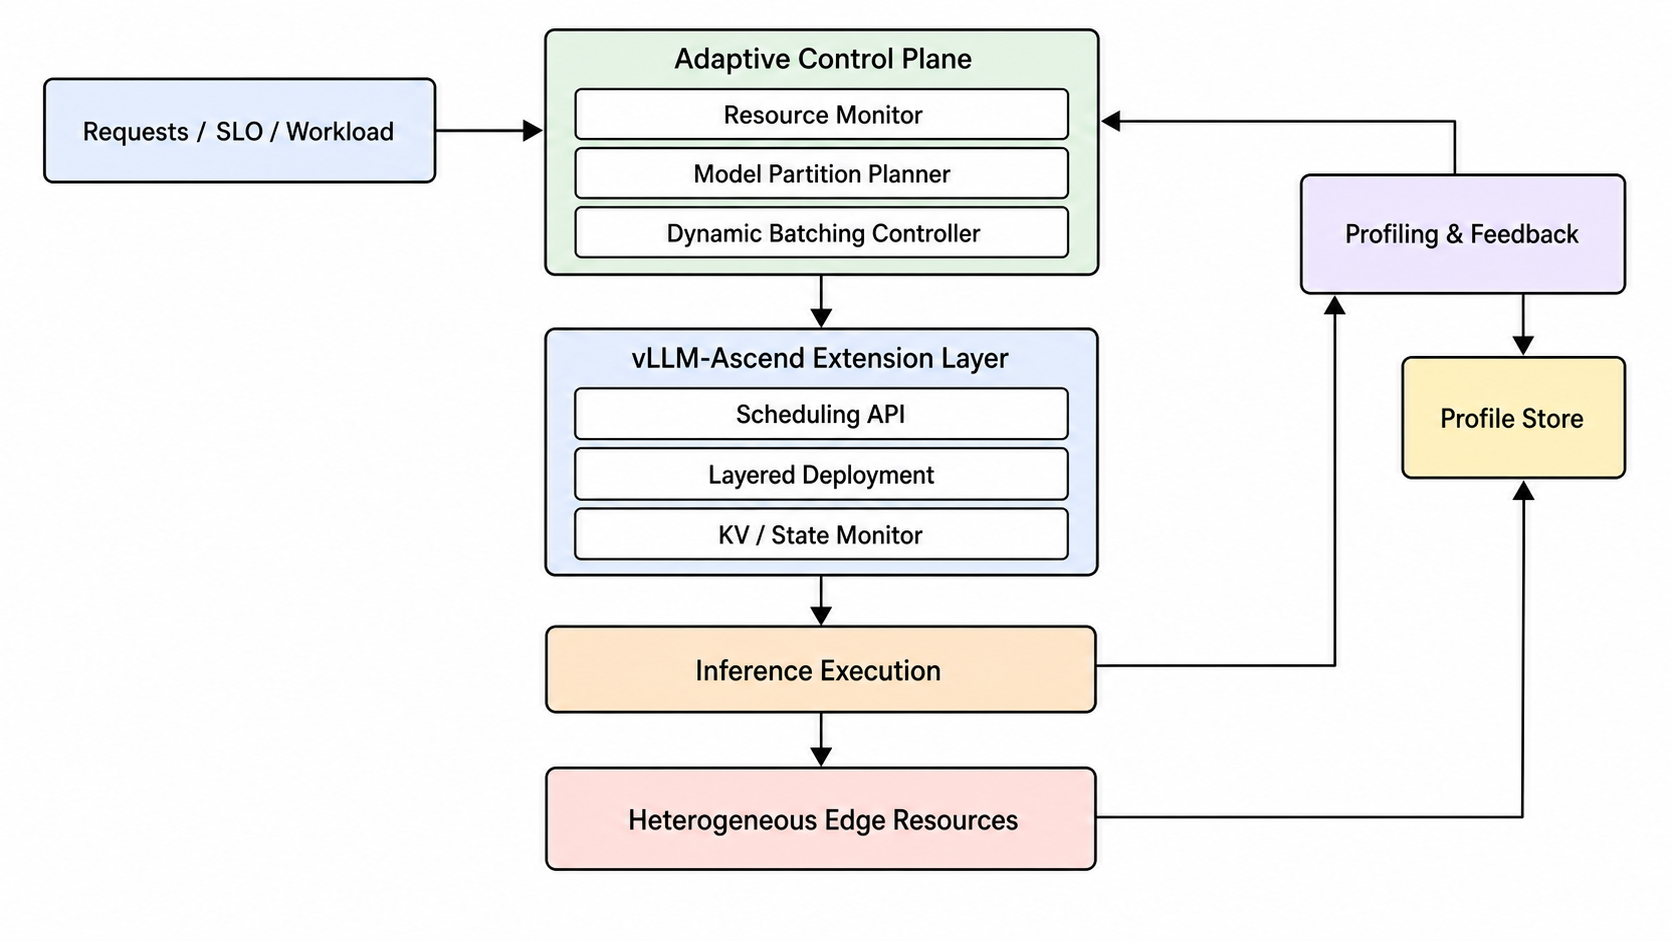
\includegraphics[width=\textwidth]{figures/ch8_engineering_architecture.png}
    \caption{面向 Ascend/CANN 验证环境的 CEC 推理工程框架}
    \label{fig:ch8-engineering-architecture}
\end{figure}

从请求路径看，业务请求从多个流量入口分别进入系统，携带 session ID、业务优先级、SLO、隐私标签、输入长度估计和上下文标识。入口层保持分布式接入方式，每个入口节点查询共享状态面并执行本地路由决策，同时接受控制面的全局约束和策略参数。入口层先判断已有 KV 或 prefix cache 位于哪个节点，再把节点显存、队列长度、链路状态和状态位置输入请求调度策略。若请求进入本地或近端实例，batching 策略决定其是否立即接纳、等待合批、进入长请求隔离队列或触发 chunked prefill；若请求需要跨节点执行，请求调度策略同时决定 KV 是本地读取、迁移、复制还是重算。

从反馈路径看，推理实例持续上报 TTFT、TPOT、ITL、E2E latency、active sequence 数、waiting queue 长度、KV block 占用、显存峰值、NPU 利用率、stage transfer time、链路 RTT/带宽和错误码。画像面将离线 profiling 与在线观测合并，形成 stage/link 代价、状态特征、动作效果、奖励和安全约束数据；状态面维护 KV owner、prefix block hash、session 入口变化和实例健康状态；控制面据此更新动态规划代价表、RL/bandit 策略、动作裁剪边界和请求路由代价。这个闭环需要为每次动作保留可追溯原因，例如选择某个切点和 placement、缩小 batch、迁移 KV 或重算 KV 时对应的状态、约束和收益估计。

\phantomsection
\subsection*{8.3 分阶段实现路线}
\addcontentsline{toc}{subsection}{8.3 分阶段实现路线}

第一阶段是 Ascend 层级切分执行能力。优先目标是让 CodeLlama34B、Qwen2-VL-7B-Instruct 等目标模型能够按连续 layer/block 切成多个 pipeline stage，并映射到 230T/64GB、70T/24GB、310P、910B4 或多机多卡 Ascend 节点上执行 \cite{huawei2026internal}。工程上需要解决四个接口：分段权重加载、stage 间 hidden state 传输、pipeline stage 启动参数和异常回退。接口稳定后，第四章的拓扑感知 layer-wise split 才能从规划结果转化为真实可部署方案，并进一步支撑 TP、EP、DP、PD 分离和 KV pool 等高阶动作。

第二阶段是 EdgeShard 风格的动态规划切分规划器。系统先对单实例、平均 layer split、固定 PP、固定 TP、PP+TP、layer sharding、context parallel、KV Cache Pool、PD 分离和 speculative decoding 等运行形态做离线 profiling，记录每层 latency、activation 大小、KV 增长、stage transfer cost、显存峰值和可支持并发，并用这些数据校准 stage 代价表、链路代价表和安全过滤器。切分规划的顺序应与第四章保持一致：先用动态规划搜索 layer-wise stage boundary、stage placement 和 pipeline balance；再判断单个 stage 是否需要叠加 TP，MoE 或组件化模型是否需要 EP，流量承载是否需要 DP；最后才把 PD 分离、KV Cache Pool 和 semantic/token-level collaboration 作为高阶候选。

第三阶段是分阶段增强的 RL/bandit 在线 batching 优化器。实现上先只训练参数自适应策略，保持框架默认请求顺序或 FIFO 不变，让策略根据并发、prompt 长度分布、KV 水位和 TTFT/TPOT/ITL 反馈调节 max running requests、max batched tokens、等待窗口、chunk size 和 prefill/decode quota。这样可以先确认收益是否来自 batching 参数本身。第二步再加入请求排序和准入控制，用 SLO slack、预测 prefill/decode 时间、KV 增长和对其他请求 ITL 的边际影响学习排序权重，使出队顺序同时反映业务紧迫度和系统边际成本。第三步再启用联合策略：短 prompt 和紧 SLO 时策略收紧 active set 与等待窗口，高并发且 slack 充足时扩大 token budget，长 prompt 或 VLM 比例升高时启用 chunked prefill 或长请求隔离，具备稳定 KV handoff 时才允许策略选择 PD 分离动作。

第四阶段是长期成本感知请求调度和 KV 管理。三个节点都应维护统一的节点负载、显存、网络和 KV 元数据；请求到达后，系统枚举目标计算节点以及 local、migrate、recompute 等状态处理动作，并先用 SLA 和 memory 约束过滤不可行动作。正常路由不只选择当前请求时延最低的节点，还要估计动作执行后 KV owner、节点负载、未来入口位置和后续 session 成本的变化。KV 管理应采用 block-level 索引和增量同步：迁移前先查询目标节点已有 prefix/KV blocks，只传输缺失部分；旧节点短期保留状态副本，以支持迁移失败、链路退化或负载突变时回退。

第五阶段是统一元数据驱动的协同控制。低频周期更新模型切分策略和服务能力布局，可按分钟级或配置变更事件触发；中频周期调节 batching 参数、admission threshold、prefill/decode quota 和实例分流，可按数秒到十秒级窗口触发；高频周期执行 request routing、workflow placement、KV migrate/recompute/local 动作和异常回退，可按单请求或 session 边界触发。三类决策必须共享同一状态视图：模型切分层输出 stage 容量和 KV handoff cost，batching 层输出队列等待和 KV 水位，请求调度层输出请求入口和状态位置。控制器重点处理三类冲突：切分带来的状态传输成本超过并行收益，batching 扩大等待窗口导致高优先级请求违约，路由因 KV 黏附远端节点造成长期跨节点通信。

\phantomsection
\subsection*{8.4 关键工程模块}
\addcontentsline{toc}{subsection}{8.4 关键工程模块}

第一个模块是 vLLM-Ascend / MindIE 接口适配层。它需要梳理模型加载、并行配置、scheduler、KV Cache 管理、metrics 暴露和错误码路径，并把底层能力转化为控制面可调用的动作接口。例如，模型切分策略输出的动作需要能够落到 stage 数、每个 stage 的 layer 范围、节点映射、tensor parallel degree、context parallel 开关、KV pool 策略和回退动作；batching 策略输出的动作需要能够落到 max running requests、max batched tokens、等待窗口、chunk size、prefill/decode quota 和 admission threshold；请求调度策略输出的动作需要能够落到目标实例、KV local/migrate/recompute、状态副本保留时间和失败回退路径。MindIE 可作为 Ascend 生态中生产化推理、调试、调优和迁移接口的参考底座 \cite{huawei2026mindie}；vLLM 的 OpenAI-compatible server 可作为服务入口和接口兼容性的参考 \cite{vllm2026openai}。

第二个模块是 Profile Store、Cost Table / Replay Buffer 与 Safety Guard。Profile Store 保存模型-硬件-拓扑的观测数据，包括 layer latency、activation、KV 增长、stage transfer cost、prefill/decode 吞吐、OOM 边界和链路状态；Cost Table 保存动态规划需要的 stage 代价、link 代价、显存约束和切换成本；Replay Buffer 保存 batching 与请求调度的状态、动作、奖励、违约和回退记录，用于离线训练、在线微调和策略回放评估；Safety Guard 保存显存上限、链路带宽下限、P99 TTFT 约束、动作冷却时间和回退条件。三者需要区分离线压测值和在线校正值：离线值用于生成初始代价表和安全边界，在线值用于修正当前窗口的动作裁剪、代价估计和奖励估计。这样可以避免系统在负载波动时盲目切换，也能避免长期使用过期画像。

第三个模块是在线策略决策器。模型切分策略只在低频周期或明显资源变化时输出动作，并设置冷却时间和最小收益阈值；batching 策略在中频周期更新参数、排序权重和准入阈值，但不直接替代 runtime 内部 token 调度；请求调度策略在高频周期处理每个 session/request 的目标节点和 KV 动作。三个决策器共享同一组约束：显存不溢出、SLA 不违约、链路带宽可承载、动作可启动、状态迁移成本可控。若安全过滤后可行动作为空，系统必须显式进入回退路径，例如降低并发、缩小 batch、回退固定 PP/TP、转发区域边缘或云端完整实例。

第四个模块是监控、审计和回退。验证环境中的算法收益必须能被复现，因此每次策略动作、batch 参数调整、请求迁移和 KV 重算都要记录触发状态、策略输出、安全过滤结果、奖励估计、最终动作和实际结果。监控指标至少包括 P90/P99 TTFT、TPOT、ITL、平均 E2E latency、SLA violation、满足 SLA 的 rps、最高并发用户数、显存峰值、OOM 次数、NPU 利用率、KV 命中率、状态迁移量和回退次数。对外报告时，应能区分收益来自层级切分策略、batching 参数自适应、请求排序策略、KV 迁移还是三者协同。

\phantomsection
\subsection*{8.5 验证路线}
\addcontentsline{toc}{subsection}{8.5 验证路线}

验证应按能力递进组织，先验证执行底座，再验证单类策略，最后验证协同闭环。第一组实验验证 Ascend 层级切分执行能力：比较单实例、平均 layer split、固定 PP/TP 和拓扑感知 layer-wise split，观察 OOM、P99 TTFT、TPOT、stage bubble、stage transfer time 和满足 SLA 的并发用户数。该组实验回答的是“Ascend 推理栈是否已经具备可执行的层级切分底座”。

第二组实验验证动态规划模型切分策略：在完成 profiling、stage/link 代价表和安全边界校准后，比较平均切分、固定 PP/TP、负载感知 placement、启发式拓扑感知 layer-wise split、EdgeShard 风格动态规划切分、动态规划加安全过滤和收益阈值。重点指标是满足 SLA 的请求处理数、最高并发用户数、显存峰值、通信开销、不可执行方案比例、pipeline bubble 和回退次数。这里的目标与第四章一致：相对于多节点平均切分基线，验证 goodput 和 SLA-constrained concurrency 是否有稳定提升 \cite{huawei2026internal}。

第三组实验验证 RL/bandit 在线 batching 优化器：先比较固定参数、离线调优参数、contextual bandit 和 actor-critic 参数自适应；再比较 FIFO、EDF/slack baseline、priority queue、边际代价排序和 RL 学习到的排序权重；最后在短 prompt、长 prompt、VLM 和多优先级混合 workload 上测试联合策略。指标应覆盖满足 SLA 的请求处理速度、平均 E2E latency、P99 TTFT、ITL 抖动、高优先级请求违约率、普通请求饥饿比例、策略切换次数和回退次数。

第四组实验验证长期成本感知请求调度和 KV 管理：比较就近执行、当前最小时延 Greedy、长期成本路由、长期成本路由加 block-level KV 管理。除 TTFT、E2E latency、吞吐和并发数外，还要统计用户移动后的累计通信时延、请求转发次数、KV 迁移/重算次数、状态传输量、prefix/KV 命中率和 session 节点切换次数。该组实验用于说明为什么 CEC 中的请求调度不能只看当前节点负载。

第五组实验验证协同控制：分别启用第四章切分策略、第五章 batching 策略和第六章请求调度但不共享状态，作为独立算法组合基线；再启用统一元数据但不做长期预测；最后启用完整的低频部署策略、中频 batching 策略、高频请求/状态路由闭环。扰动项包括链路带宽、RTT、可用显存、长 prompt 比例、移动用户比例和请求优先级分布。最终报告应同时给出性能收益和稳定性成本，尤其是策略切换频率、策略震荡、回退次数和状态传输开销。

\phantomsection
\subsection*{8.6 小结}
\addcontentsline{toc}{subsection}{8.6 小结}

工程结论是：面向 Ascend 验证环境的 CEC LLM 推理系统应先补齐层级切分执行底座，再把模型切分、batching 和请求调度分别实现为可观测、可回退、可解释的在线决策能力。第四章对应低频的动态规划混合切分部署；第五章对应中频的分阶段 RL/bandit batching 优化器；第六章对应高频的长期成本感知请求路由和 KV 管理；第七章则把三者收敛为统一元数据驱动的分层协同控制。

这样的工程路线与现有 vLLM-Ascend 能力并不冲突。vLLM-Ascend 继续负责模型加载、算子执行、KV 管理和实例内调度；外层系统负责画像、动态规划、策略学习、状态、路由、动作裁剪和回退。只有把“可执行动作接口”和“在线状态”放在同一个闭环中，前文提出的算法建议才会从综述中的方法对比，转化为验证环境中可以部署、压测和解释的工程方案。

\input{sections/09-challenges-and-future-work}
\input{sections/10-conclusion}
\phantomsection
\section*{参考文献}
\addcontentsline{toc}{section}{参考文献}

\hypertarget{ref:1}{[1]} Y. Sheng et al., "FlexGen: High-throughput generative inference of large language models with a single GPU," in Proc. Int. Conf. Machine Learning (ICML), 2023.


\hypertarget{ref:2}{[2]} A. Borzunov et al., "Petals: Collaborative inference and fine-tuning of large models," in Proc. 61st Annu. Meeting Assoc. Comput. Linguistics (ACL), vol. 3, 2023, pp. 558-568.


\hypertarget{ref:3}{[3]} Y. Jiang et al., "HexGen: Generative inference of large language model over heterogeneous environment," in Proc. Int. Conf. Machine Learning (ICML), 2024, pp. 21946-21961.


\hypertarget{ref:4}{[4]} G.-I. Yu et al., "Orca: A distributed serving system for Transformer-based generative models," in Proc. USENIX Symp. Operating Systems Design and Implementation (OSDI), 2022, pp. 521-538.


\hypertarget{ref:5}{[5]} W. Kwon et al., "Efficient memory management for large language model serving with PagedAttention," in Proc. ACM Symp. Operating Systems Principles (SOSP), 2023, pp. 611-626.


\hypertarget{ref:6}{[6]} A. Agrawal et al., "Taming throughput-latency tradeoff in LLM inference with Sarathi-Serve," in Proc. USENIX Symp. Operating Systems Design and Implementation (OSDI), 2024, pp. 117-134.


\hypertarget{ref:7}{[7]} Y. Zhong et al., "DistServe: Disaggregating prefill and decoding for goodput-optimized large language model serving," in Proc. USENIX Symp. Operating Systems Design and Implementation (OSDI), 2024.


\hypertarget{ref:8}{[8]} L. Zheng et al., "SGLang: Efficient execution of structured language model programs," in Proc. Adv. Neural Inf. Process. Syst. (NeurIPS), 2024.


\hypertarget{ref:9}{[9]} NVIDIA, "TensorRT-LLM documentation," 2026. [Online]. Available: \href{https://nvidia.github.io/TensorRT-LLM/}{\url{https://nvidia.github.io/TensorRT-LLM/}}


\hypertarget{ref:10}{[10]} NVIDIA, "Triton Inference Server: Dynamic batcher," 2026. [Online]. Available: \href{https://docs.nvidia.com/deeplearning/triton-inference-server/}{\url{https://docs.nvidia.com/deeplearning/triton-inference-server/}}


\hypertarget{ref:11}{[11]} Hugging Face, "Text Generation Inference documentation," 2026. [Online]. Available: \href{https://huggingface.co/docs/text-generation-inference/}{\url{https://huggingface.co/docs/text-generation-inference/}}


\hypertarget{ref:12}{[12]} Y. Jiang, R. Yan, and B. Yuan, "HexGen-2: Disaggregated generative inference of LLMs in heterogeneous environment," in Proc. Int. Conf. Learn. Representations (ICLR), 2025.


\hypertarget{ref:13}{[13]} S. Duan, D. Wang, J. Ren, F. Lyu, Y. Zhang, H. Wu, and X. Shen, "Distributed artificial intelligence empowered by end-edge-cloud computing: A survey," IEEE Communications Surveys \& Tutorials, vol. 25, no. 1, pp. 591-624, 2023.


\hypertarget{ref:14}{[14]} Y. Huang et al., "GPipe: Efficient training of giant neural networks using pipeline parallelism," in Proc. Adv. Neural Inf. Process. Syst. (NeurIPS), 2019, pp. 103-112.


\hypertarget{ref:15}{[15]} D. Narayanan et al., "Efficient large-scale language model training on GPU clusters using Megatron-LM," in Proc. Int. Conf. High Performance Computing, Networking, Storage and Analysis (SC), 2021.


\hypertarget{ref:16}{[16]} L. Zheng et al., "Alpa: Automating inter- and intra-operator parallelism for distributed deep learning," in Proc. USENIX Symp. Operating Systems Design and Implementation (OSDI), 2022, pp. 559-578.


\hypertarget{ref:17}{[17]} R. Y. Aminabadi et al., "DeepSpeed-Inference: Enabling efficient inference of transformer models at unprecedented scale," in Proc. Int. Conf. High Performance Computing, Networking, Storage and Analysis (SC), 2022.


\hypertarget{ref:18}{[18]} P. Patel et al., "Splitwise: Efficient generative LLM inference using phase splitting," in Proc. ACM/IEEE Int. Symp. Computer Architecture (ISCA), 2024, pp. 118-132.


\hypertarget{ref:19}{[19]} B. Sun et al., "Llumnix: Dynamic scheduling for large language model serving," in Proc. USENIX Symp. Operating Systems Design and Implementation (OSDI), 2024, pp. 173-191.


\hypertarget{ref:20}{[20]} R. Prabhu, A. Nayak, J. Mohan, R. Ramjee, and A. Panwar, "vAttention: Dynamic memory management for serving LLMs without PagedAttention," in Proc. ACM Int. Conf. Architectural Support for Programming Languages and Operating Systems (ASPLOS), 2025, pp. 1133-1150.


\hypertarget{ref:21}{[21]} R. Qin et al., "Mooncake: Trading more storage for less computation -- A KVCache-centric architecture for serving LLM chatbot," in Proc. USENIX Conf. File and Storage Technologies (FAST), 2025, pp. 155-170.


\hypertarget{ref:22}{[22]} Y. Liu et al., "CacheGen: KV cache compression and streaming for fast large language model serving," in Proc. ACM SIGCOMM, 2024, pp. 38-56.


\hypertarget{ref:23}{[23]} V. Srivatsa et al., "Preble: Efficient distributed prompt scheduling for LLM serving," in Proc. Int. Conf. Learn. Representations (ICLR), 2025.


\hypertarget{ref:24}{[24]} B. Gao et al., "Cost-efficient large language model serving for multi-turn conversations with CachedAttention," in Proc. USENIX Annu. Tech. Conf. (ATC), 2024, pp. 111-126.


\hypertarget{ref:25}{[25]} T. Ouyang, Z. Zhou, and X. Chen, "Follow Me at the Edge: Mobility-aware dynamic service placement for mobile edge computing," IEEE J. Sel. Areas Commun., vol. 36, no. 10, pp. 2333-2345, Oct. 2018.


\hypertarget{ref:26}{[26]} Y. Sheng et al., "Fairness in serving large language models," in Proc. USENIX Symp. Operating Systems Design and Implementation (OSDI), 2024, pp. 965-988.



\hypertarget{ref:27}{[27]} S. Ye, B. Ouyang, L. Zeng, T. Qian, X. Chu, J. Tang, and X. Chen, "Jupiter: Fast and Resource-Efficient Collaborative Inference of Generative LLMs on Edge Devices," in Proc. IEEE INFOCOM, 2025.

\hypertarget{ref:28}{[28]} B. Zhang, J. Zhang, J. Hou, and Y. Wang, "TensAllo: Adaptive Deployment of LLMs on Resource-Constrained Heterogeneous Edge Devices," in Proc. IEEE INFOCOM, 2025.

\hypertarget{ref:29}{[29]} M. Zhang, J. Cao, X. Shen, and Z. Cui, "EdgeShard: Efficient LLM Inference via Collaborative Edge Computing," IEEE Internet of Things Journal, 2025.

\hypertarget{ref:30}{[30]} S. Ye et al., "Resource-Efficient Collaborative Edge Transformer Inference With Hybrid Model Parallelism," IEEE Transactions on Mobile Computing, vol. 24, no. 10, pp. 10945-10962, 2025.

\hypertarget{ref:31}{[31]} J. Du, Y. Wei, S. Ye, J. Jiang, X. Chen, D. Huang, and Y. Lu, "Co-Designing Transformer Architectures for Distributed Inference With Low Communication," IEEE Transactions on Parallel and Distributed Systems, vol. 36, no. 4, 2025.

\hypertarget{ref:32}{[32]} X. Feng et al., "E2LLM: Structure-Guided Efficient Inference for LLMs in Distributed Edge-IoT Environments," IEEE Transactions on Mobile Computing, 2026.

\hypertarget{ref:33}{[33]} Y. Lin, S. Peng, C. Lu, C. Xu, and K. Ye, "FlexPipe: Adapting Dynamic LLM Serving Through Inflight Pipeline Refactoring in Fragmented Serverless Clusters," in Proc. EuroSys, 2026.

\hypertarget{ref:34}{[34]} G. Qu, T. Li, Q. Chen, X. Chen, and S. Zhou, "SLIDE: Simultaneous Model Downloading and Inference at the Wireless Network Edge," IEEE Transactions on Mobile Computing, 2026.

\hypertarget{ref:35}{[35]} D. Xu et al., "EdgeLLM: Fast On-Device LLM Inference With Speculative Decoding," IEEE Transactions on Mobile Computing, vol. 24, no. 4, pp. 3256-3271, 2025.

\hypertarget{ref:36}{[36]} F. Chen, P. Li, T. H. Luan, Z. Su, and J. Deng, "SPIN: Accelerating Large Language Model Inference with Heterogeneous Speculative Models," in Proc. IEEE INFOCOM, 2025.

\hypertarget{ref:37}{[37]} X. Miao et al., "SpecInfer: Accelerating Large Language Model Serving with Tree-based Speculative Inference and Verification," in Proc. ACM Int. Conf. Architectural Support for Programming Languages and Operating Systems (ASPLOS), 2024.

\hypertarget{ref:38}{[38]} R. Kong et al., "SwapMoE: Serving Off-the-shelf MoE-based Large Language Models with Tunable Memory Budget," in Proc. Annu. Meeting Assoc. Comput. Linguistics (ACL), 2024.

\hypertarget{ref:39}{[39]} H. Yu, X. Cui, H. Zhang, H. Wang, and H. Wang, "Taming Latency-Memory Trade-Off in MoE-Based LLM Serving via Fine-Grained Expert Offloading," in Proc. EuroSys, 2026.

\hypertarget{ref:40}{[40]} L. Xue, Y. Fu, Z. Lu, C. Sun, L. Mai, and M. Marina, "MoE-Infinity: Efficient MoE Inference on Personal Machines with Sparsity-Aware Expert Cache," in Proc. Int. Conf. Machine Learning (ICML), 2025.

\hypertarget{ref:41}{[41]} R. Hwang et al., "Pre-gated MoE: An Algorithm-System Co-Design for Fast and Scalable MoE Inference," in Proc. ACM/IEEE Int. Symp. Computer Architecture (ISCA), 2024.

\hypertarget{ref:42}{[42]} R. Yi, L. Guo, S. Wei, A. Zhou, S. Wang, and M. Xu, "EdgeMoE: Empowering Sparse Large Language Models on Mobile Devices," IEEE Transactions on Mobile Computing, 2025.

\hypertarget{ref:43}{[43]} N. Xue et al., "WDMoE: Wireless Distributed Mixture of Experts for Large Language Models," IEEE Transactions on Wireless Communications, 2025.

\hypertarget{ref:44}{[44]} R. Lu, Y. Liu, and D. Wang, "P4LLM: Protecting Embedding Privacy against Model Inversion Attacks for EaaS LLM Serving via Token-wise Partition and Perturbation," IEEE Transactions on Mobile Computing, 2026.

\hypertarget{ref:45}{[45]} W. Zhang, Z. Wu, Y. Mu, R. Ning, B. Liu, N. Sarda, M. Lee, and F. Lai, "JITServe: SLO-aware LLM Serving with Imprecise Request Information," in Proc. USENIX Symp. Networked Systems Design and Implementation (NSDI), 2026.

\hypertarget{ref:46}{[46]} K. Hong et al., "SOLA: Optimizing SLO Attainment for Large Language Model Serving with State-Aware Scheduling," in Proc. Conf. Machine Learning and Systems (MLSys), 2025.

\hypertarget{ref:47}{[47]} A. Patke et al., "One Queue Is All You Need: Resolving Head-of-Line Blocking in Large Language Model Serving," in Proc. Workshop on Cloud Intelligence/AIOps (AIOps@ASPLOS), 2024.

\hypertarget{ref:48}{[48]} N. Ling, G. Chen, and L. Zhong, "TimelyLLM: Segmented LLM Serving System for Time-sensitive Robotic Applications," in Proc. ACM MobiSys, 2026.

\hypertarget{ref:49}{[49]} B. Wu et al., "FastServe: Iteration-Level Preemptive Scheduling for Large Language Model Inference," in Proc. USENIX Symp. Networked Systems Design and Implementation (NSDI), 2026.

\hypertarget{ref:50}{[50]} J. Chen et al., "TokenFlow: Responsive LLM Text Streaming Serving under Request Burst via Preemptive Scheduling," in Proc. EuroSys, 2026.

\hypertarget{ref:51}{[51]} K. Zhu et al., "NanoFlow: Towards Optimal Large Language Model Serving Throughput," in Proc. USENIX Symp. Operating Systems Design and Implementation (OSDI), 2025.

\hypertarget{ref:52}{[52]} C. Ruan et al., "Libra: Flexible Request Partitioning and Scheduling for Serving Unbalanced and Dynamic LLM Workloads," in Proc. USENIX Symp. Networked Systems Design and Implementation (NSDI), 2026.

\hypertarget{ref:53}{[53]} Y. Shen, Y. Zhang, and D. Yuan, "A Hybrid Online and Offline Requests Inference Serving System for LLM in Private Computer Environment," IEEE Transactions on Computers, vol. 75, no. 3, 2026.

\hypertarget{ref:54}{[54]} Z. Li et al., "AdaServe: Accelerating Multi-SLO LLM Serving with SLO-Customized Speculative Decoding," in Proc. EuroSys, 2026.

\hypertarget{ref:55}{[55]} J. Yang, Q. Wu, Z. Feng, Z. Zhou, D. Guo, and X. Chen, "Quality-of-Service Aware LLM Routing for Edge Computing with Multiple Experts," IEEE Transactions on Mobile Computing, 2025.

\hypertarget{ref:56}{[56]} Y. Li, J. Guo, Z. Tang, X. Ding, J. Wang, T. Wang, and W. Jia, "Cloud-Edge System for Scheduling Unpredictable LLM Requests With Combinatorial Bandit," IEEE Transactions on Services Computing, vol. 18, no. 6, pp. 3567-3580, 2025.

\hypertarget{ref:57}{[57]} I. Ong et al., "RouteLLM: Learning to Route LLMs from Preference Data," in Proc. Int. Conf. Learn. Representations (ICLR), 2025.

\hypertarget{ref:58}{[58]} F. Wu and S. Silwal, "PORT: Efficient Training-Free Online Routing for High-Volume Multi-LLM Serving," in Proc. Adv. Neural Inf. Process. Syst. (NeurIPS), 2025.

\hypertarget{ref:59}{[59]} Y. He, J. Fang, F. R. Yu, and V. C. Leung, "Large Language Models (LLMs) Inference Offloading and Resource Allocation in Cloud-Edge Computing: An Active Inference Approach," IEEE Transactions on Mobile Computing, vol. 23, no. 12, pp. 11253-11264, 2024.

\hypertarget{ref:60}{[60]} X. Xu, G. Feng, Y. Liu, S. Qin, J. Wang, and Y. Wang, "Joint Inference Offloading and Model Caching for Small and Large Language Model Collaboration," IEEE Transactions on Mobile Computing, vol. 25, no. 2, 2026.

\hypertarget{ref:61}{[61]} A. Ghosh, N. Sharma, S. Mishra, R. Misra, and S. K. Das, "MGCO: Mobility-Aware Generative Computation Offloading in Edge-Cloud Systems," IEEE Transactions on Services Computing, vol. 19, no. 1, pp. 477-490, 2026.

\hypertarget{ref:62}{[62]} Y. Yue et al., "MasRouter: Learning to Route LLMs for Multi-Agent Systems," in Proc. Annu. Meeting Assoc. Comput. Linguistics (ACL), 2025.

\hypertarget{ref:63}{[63]} S. Nielsen, E. Cetin, P. Schwendeman, Q. Sun, J. Xu, and Y. Tang, "Learning to Orchestrate Agents in Natural Language with the Conductor," in Proc. Int. Conf. Learn. Representations (ICLR), 2026.

\hypertarget{ref:64}{[64]} J. Zhang et al., "AFlow: Automating Agentic Workflow Generation," in Proc. Int. Conf. Learn. Representations (ICLR), 2025.

\hypertarget{ref:65}{[65]} X. Chen, J. Cao, Y. Sahni, M. Zhang, Z. Liang, and L. Yang, "Mobility-Aware Dependent Task Offloading in Edge Computing: A Digital Twin-Assisted Reinforcement Learning Approach," IEEE Transactions on Mobile Computing, vol. 24, no. 4, pp. 2979-2994, 2025.

\hypertarget{ref:66}{[66]} J. Jiang et al., "Efficient KV Cache Spillover Management on Memory-Constrained GPU for LLM Inference," IEEE Transactions on Parallel and Distributed Systems, vol. 37, no. 1, 2026.

\hypertarget{ref:67}{[67]} S. Gao, Q. Wang, S. Zeng, Y. Lu, and J. Shu, "Weaver: Efficient Multi-LLM Serving with Attention Offloading," in Proc. USENIX Annu. Tech. Conf. (ATC), 2025, pp. 587-595.

\hypertarget{ref:68}{[68]} M. Xu, D. Niyato, and C. G. Brinton, "Serving Long-Context LLMs at the Mobile Edge: Test-Time Reinforcement Learning-Based Model Caching and Inference Offloading," IEEE/ACM Transactions on Networking, vol. 34, pp. 3808-3823, 2026.

\hypertarget{ref:69}{[69]} J. Wang et al., "Context-Aware AIGC Service Migration in Edge Intelligence Networks via Transformer DRL," IEEE Transactions on Services Computing, vol. 19, no. 2, pp. 1020-1033, 2026.


\hypertarget{ref:70}{[70]} LMDeploy Team, "LMDeploy documentation," 2026. [Online]. Available: \href{https://lmdeploy.readthedocs.io/}{\url{https://lmdeploy.readthedocs.io/}}

\hypertarget{ref:71}{[71]} A. Du, J. Jia, S. Dustdar, J. Chen, and X. Wang, "Online Service Placement, Task Scheduling, and Resource Allocation in Hierarchical Collaborative MEC Systems," IEEE Transactions on Services Computing, vol. 18, no. 2, pp. 983-997, 2025.

\hypertarget{ref:72}{[72]} X. Zhuang, J. Wu, H. Wu, T. Zhang, and L. Gao, "Joint Optimization of Model Inferencing and Task Offloading for MEC-Empowered Large Vision Model Services," in Proc. IEEE INFOCOM, 2025.

\hypertarget{ref:73}{[73]} Z. Zhou et al., "A Survey on Efficient Inference for Large Language Models," arXiv:2404.14294, 2024.

\hypertarget{ref:74}{[74]} R. Zhen et al., "Taming the Titans: A Survey of Efficient LLM Inference Serving," in Proc. Int. Natural Language Generation Conf. (INLG), 2025, pp. 522-541.

\hypertarget{ref:75}{[75]} J. Pan and G. Li, "A Survey of LLM Inference Systems," arXiv:2506.21901, 2025.






\hypertarget{ref:76}{[76]} 华为，《边缘 AI 计算技术合作项目资料》，2026.

\hypertarget{ref:77}{[77]} vLLM Ascend Team, "vLLM Ascend documentation," 2026. [Online]. Available: \href{https://docs.vllm.ai/projects/ascend/en/latest/}{\url{https://docs.vllm.ai/projects/ascend/en/latest/}}

\hypertarget{ref:78}{[78]} vLLM Ascend Team, "vLLM Ascend installation guide," 2026. [Online]. Available: \href{https://docs.vllm.ai/projects/ascend/en/latest/installation.html}{\url{https://docs.vllm.ai/projects/ascend/en/latest/installation.html}}

\hypertarget{ref:79}{[79]} vLLM Ascend Team, "vLLM Ascend features," 2026. [Online]. Available: \href{https://docs.vllm.ai/projects/ascend/en/latest/features/}{\url{https://docs.vllm.ai/projects/ascend/en/latest/features/}}

\hypertarget{ref:80}{[80]} vLLM Ascend Team, "KV Cache Pool," 2026. [Online]. Available: \href{https://docs.vllm.ai/projects/ascend/en/latest/features/kv_cache_pool.html}{\url{https://docs.vllm.ai/projects/ascend/en/latest/features/kv_cache_pool.html}}

\hypertarget{ref:81}{[81]} vLLM Ascend Team, "Speculative decoding," 2026. [Online]. Available: \href{https://docs.vllm.ai/projects/ascend/en/latest/features/spec_decode.html}{\url{https://docs.vllm.ai/projects/ascend/en/latest/features/spec_decode.html}}

\hypertarget{ref:82}{[82]} Huawei Ascend, "Model inference," 2026. [Online]. Available: \href{https://www.hiascend.com/software/model-inference}{\url{https://www.hiascend.com/software/model-inference}}

\hypertarget{ref:83}{[83]} vLLM Project, "OpenAI-compatible server," 2026. [Online]. Available: \href{https://docs.vllm.ai/en/latest/serving/openai_compatible_server.html}{\url{https://docs.vllm.ai/en/latest/serving/openai_compatible_server.html}}




\end{document}
